\chapter{Experiments}
\label{chap:experiments}
This chapter presents the experiments designed to evaluate the system described in chapter \autoref{chap:methods}.
The chapter is structured as follows:
\autoref{sec:exp-setup} specifies the setup used for the class incremental learning task;
\autoref{sec:exp-cil} discusses the experiments related to the CIL model;
\autoref{sec:exp-kd} describes the experiments aimed to reduce the number of model parameters using Knowledge Distillation (KD);
\autoref{sec:exp-det} discusses the experiments related to the logo detector;
the chapter ends in \autoref{sec:exp-end2end} presenting the results of experiments combining the logo detector and the CIL classifier.

\section{Setup}
\label{sec:exp-setup}
The developed system is tested considering two different CIL setups: the first consists of a subset of 100 classes out of 2993 in the dataset; the second tests the model's scaling capabilities using the entire dataset.
In detail, the CIL setups are defined as follows:
\begin{enumerate}
    \item \textbf{100 Classes}: from the initial dataset 100 classes are extracted. 
    For experiments, a distinction is made between the case where classes are randomly sampled or the 100 classes with the highest number of images are taken.
    
    Of these 100 classes, 30 are used for the initial task, then the remaining 70 are used 10 at a time through 7 iterations of incremental learning.

    \item \textbf{2993 Classes (entire dataset)}: for experiments considering the entire dataset, the first 1000 classes are used for the initial task, followed by 8 iterations of incremental learning, each of which adds 250 new classes.
\end{enumerate}

Training, validation and test sets are built from the individual classes. For each class, the instances are divided as follows:
\begin{itemize}
    \item \textbf{Training set}: 70 \%
    \item \textbf{Validation set}: 10 \%
    \item \textbf{Test set}: 20 \%
\end{itemize}


\section{Classifier: CIL model}
\label{sec:exp-cil}
Top-k accuracy is used to evaluate the performance of the CIL model, focusing on cases where $k=1$ and $k=5$.
Using this performance metric, a classification is considered correct if the label is present among the first $k$ predictions to which the model assigns the highest probability.
Accuracy is then calculated as the percentage of correct predictions.

\subsection{100 Classes}
\subsubsection{100 Classes randomly sampled}
For the first experiments, the 100 classes are randomly sampled from the 2993 classes in the dataset.

%, then the classifier is evaluated on the test set according to the CIL setup described in \autoref{sec:exp-setup}. 


As described in \autoref{sec:der-algorithm}, the DER algorithm saves some samples of the 'old' classes and reuses them during incremental learning iterations.
In the following experiments, the memory dedicated to each old class is 100 samples.

The following experiments aim to compare ResNet-34 and ResNet-50 architectures used as feature extractors $\mathcal{F}_t$ (see \autoref{sec:der-algorithm}), distinguishing between cases where CNNs are pre-trained or not on ImageNet.
For these experiments, the optimizer is SGD and neither model regularization by dropout layer nor data augmentation are used.

The results of the experiments are shown in \autoref{fig:exp1} and in \autoref{table:exp1}, which report the top-1 and top-5 accuracy calculated on the test set as the CIL tasks vary. As we can see, the pre-trained CNNs perform better, but there is not much difference between ResNet-34 and ResNet-50.

Based on these results, the architecture chosen for the next experiments is ResNet-34 (so that the network is slightly smaller than ResNet-50) with its weights pre-trained on ImageNet.

\begin{figure}[H]
    \centering
	\subfloat[\centering Top-1 accuracy]{{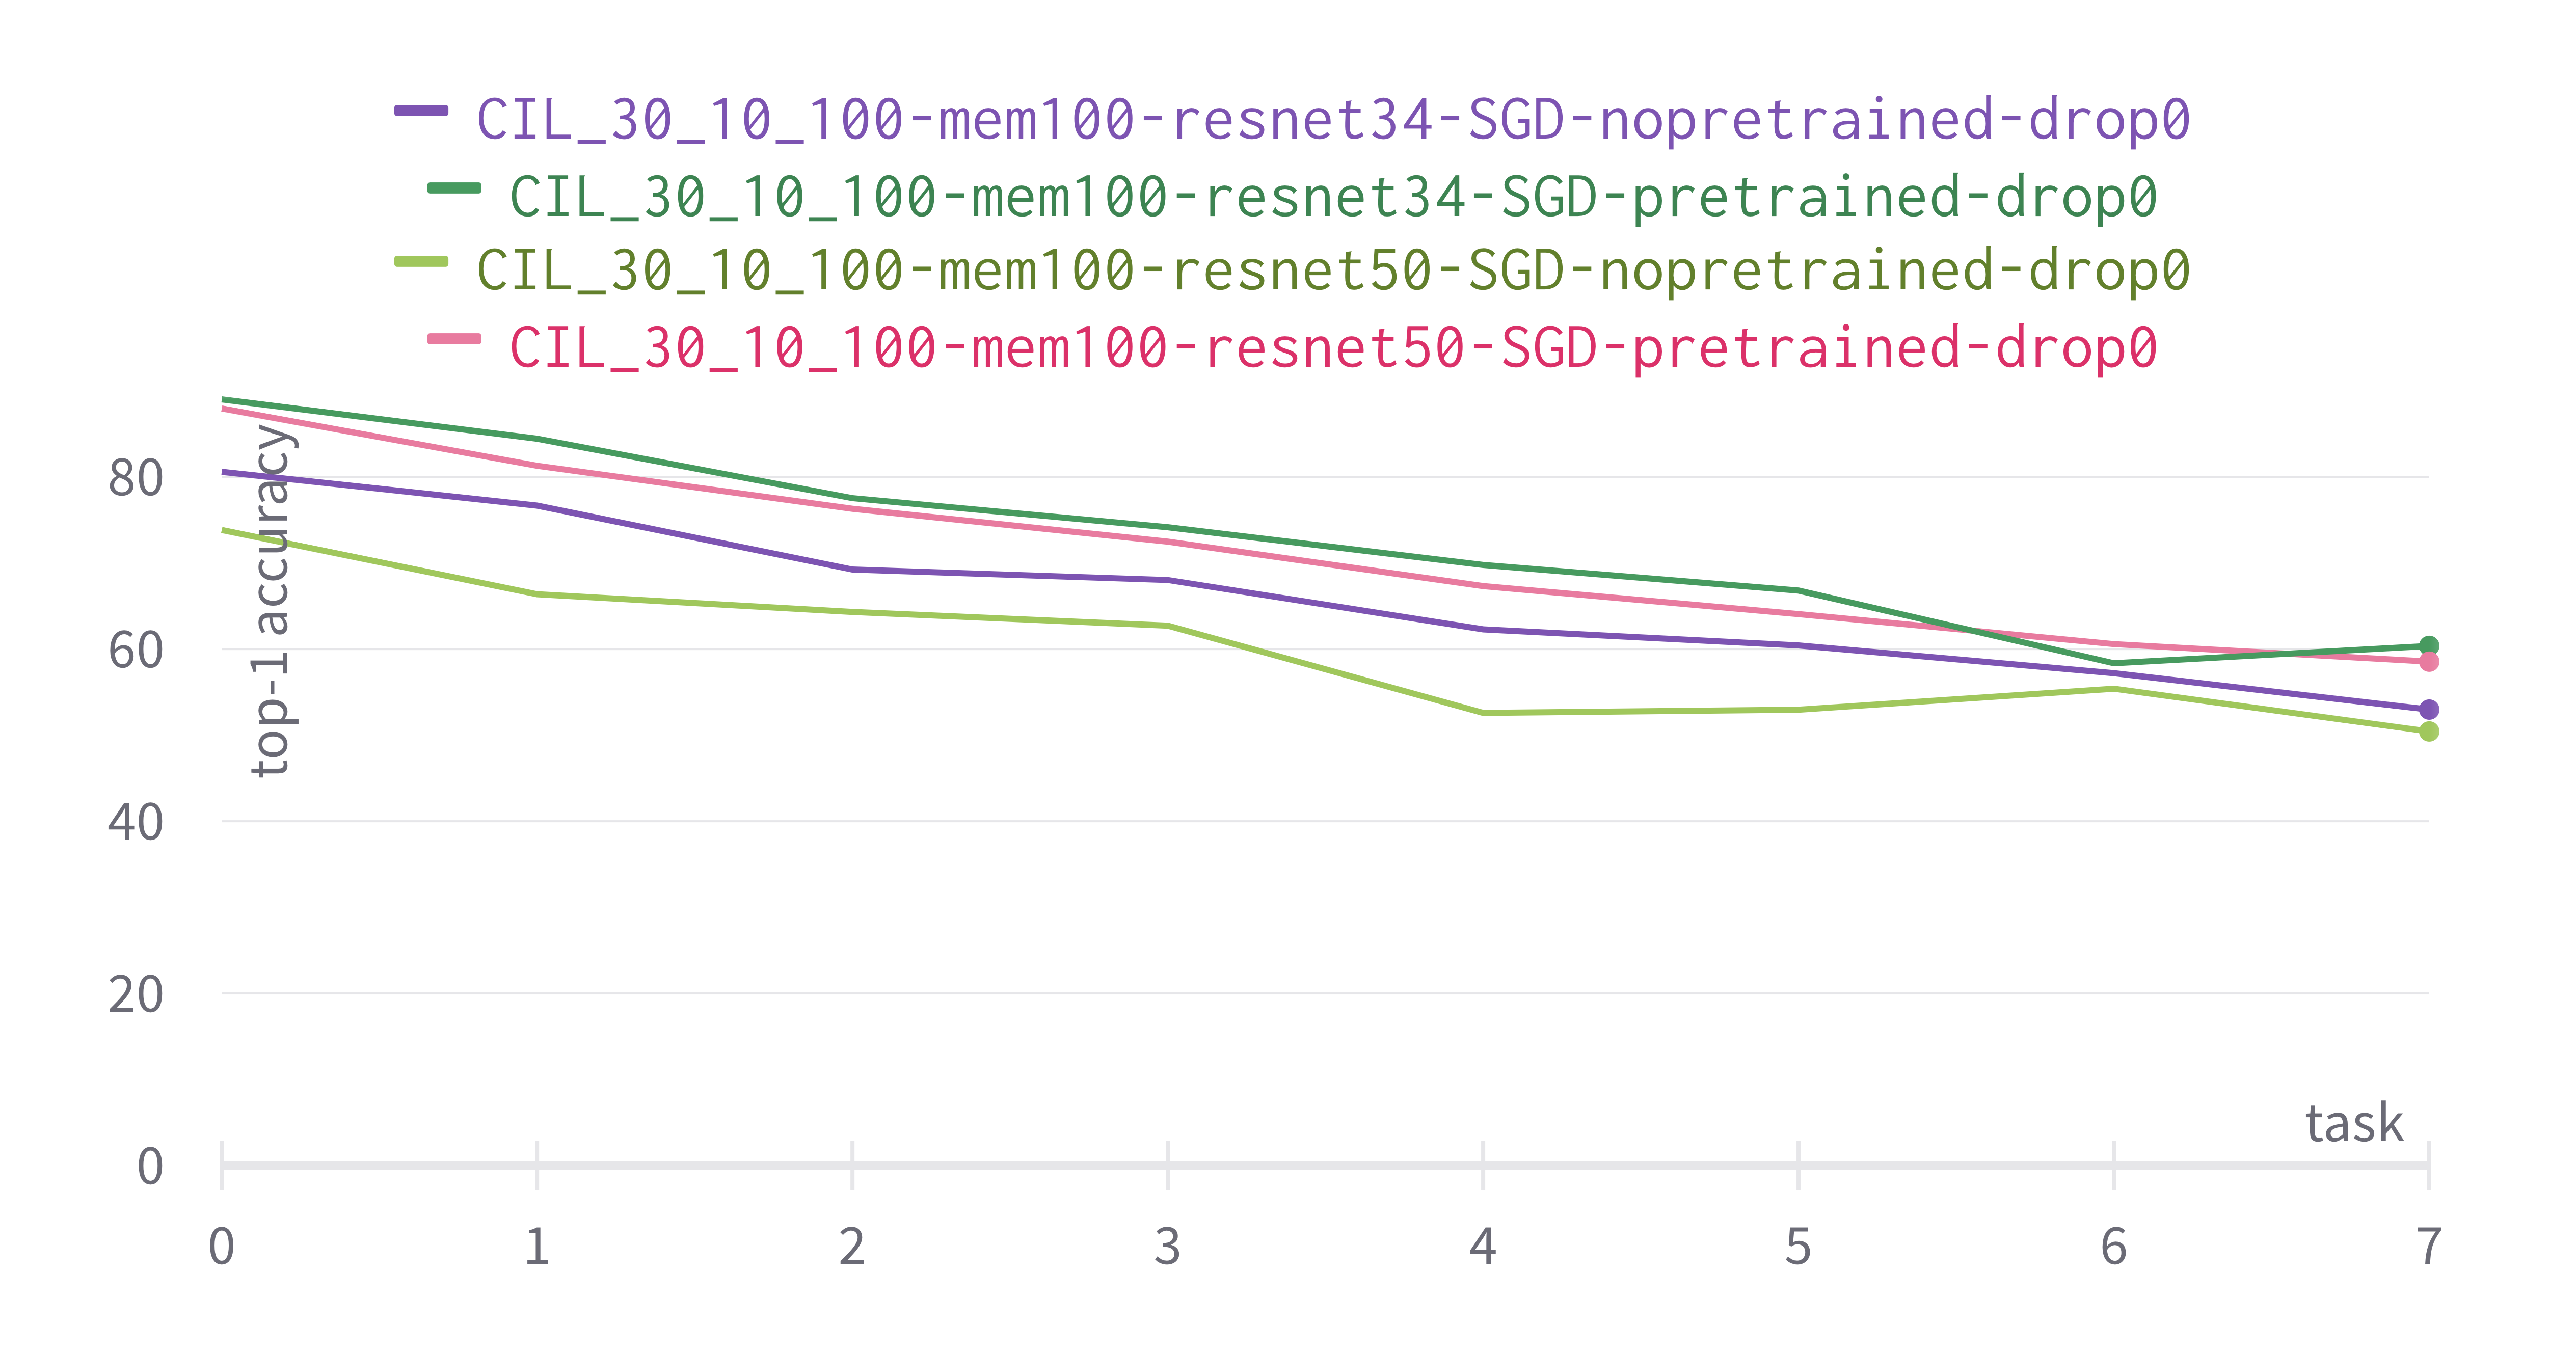
\includegraphics[width=0.50\textwidth]{images/exp/exp1-top1.png} }}%
    %\qquad
    \subfloat[\centering Top-5 accuracy]{{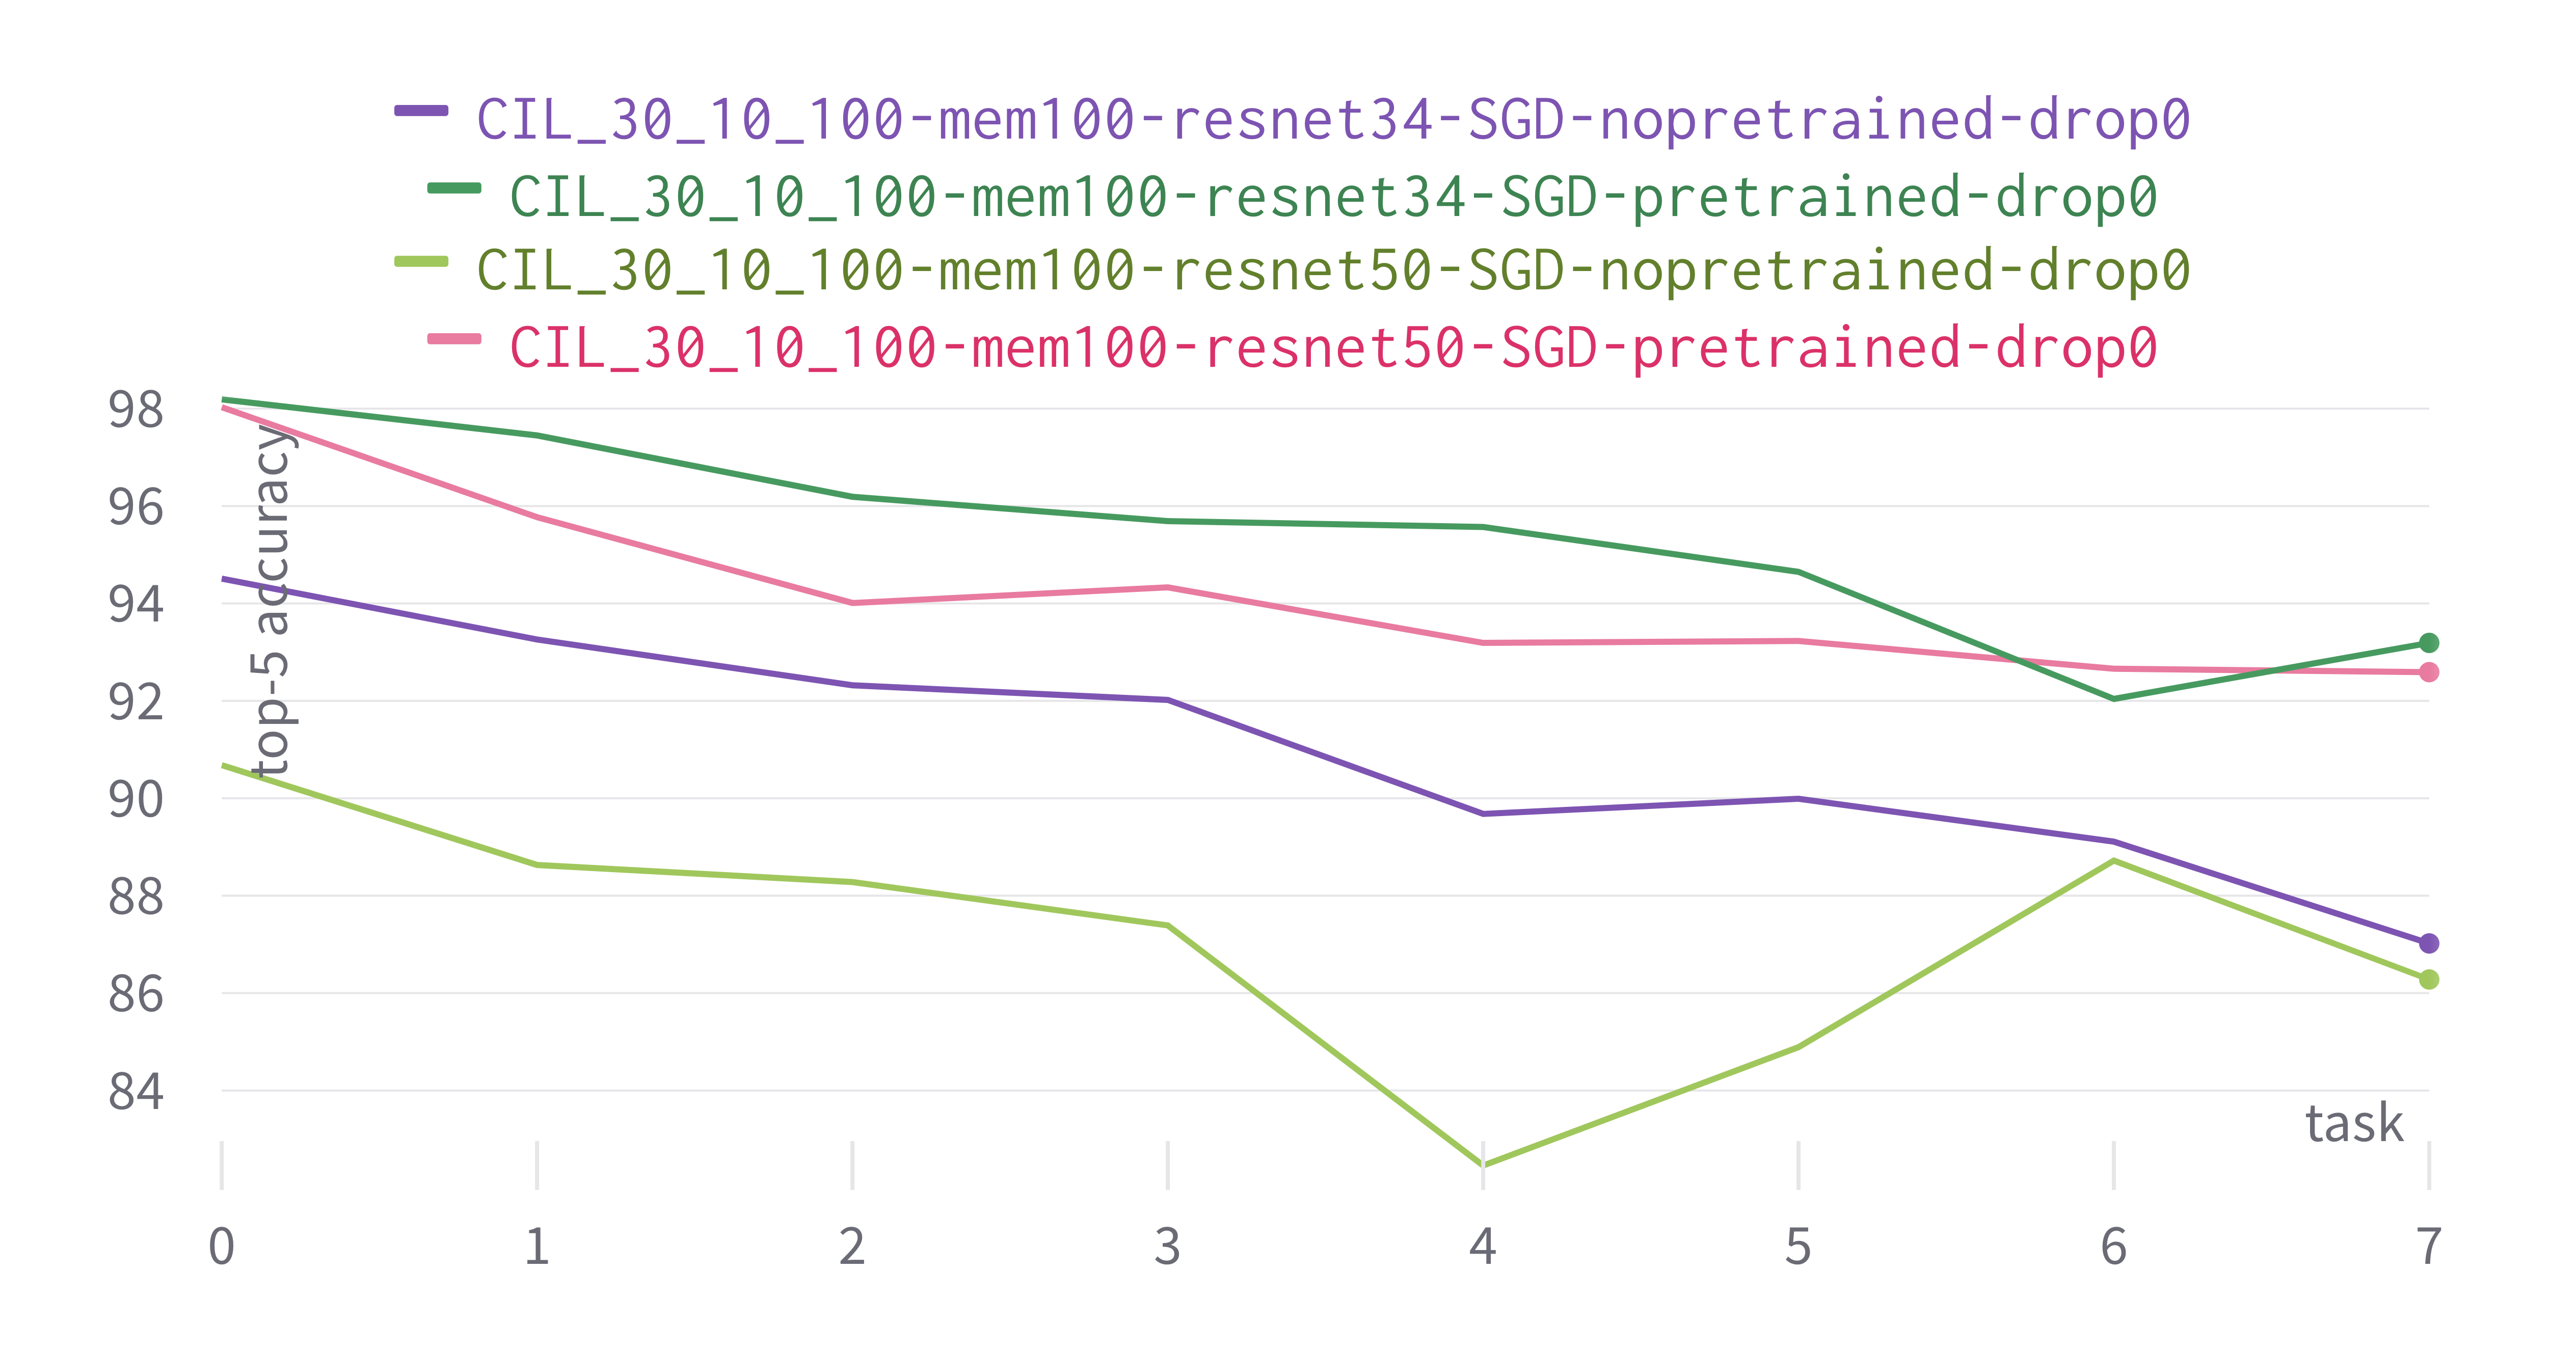
\includegraphics[width=0.50\textwidth]{images/exp/exp1-top5.png} }}%
    \caption{Top-1 and top-5 accuracy of models on the test set at different CIL tasks.}%
	\label{fig:exp1}%
\end{figure}

\begin{table}[H]
    \centering
    \centerline{
    \begin{tabular}{c|c|c|c|c}
        \hline
        \textbf{Model} &
        \textbf{Backbone} &
        \textbf{Pre-trained} &
        \textbf{Top-1} & 
        \textbf{Top-5} \\
        \textbf{name} &
        &
        &
        \textbf{acc. (\%)} & 
        \textbf{acc. (\%)} \\
        \hline
        \hline
resnet34-SGD-nopretrained-drop0 &ResNet-34&no& 52.97 & 87.02\\
resnet34-SGD-pretrained-drop0 &ResNet-34&yes& \textbf{60.37} & \textbf{93.19}\\
resnet50-SGD-nopretrained-drop0 &ResNet-50&no& 50.43 & 86.28\\
resnet50-SGD-pretrained-drop0 &ResNet-50&yes& 58.54 & 92.59\\
        \hline        
    \end{tabular}}
    \caption{Top-1 and top-5 accuracy of models at task 7.}
    \label{table:exp1}
\end{table}

Other useful insights can be derived from the training history of a task (e.g. task 7) reporting the top-1 accuracy on the training and validation set.
Indeed, as can be seen from \autoref{fig:exp1-train_val} the accuracy on the training set is much higher than the one on the validation set, which is a clear sign of overfitting of the model.

\begin{figure}[H]
    \centering
    \subfloat[\centering Accuracy on the training set]{{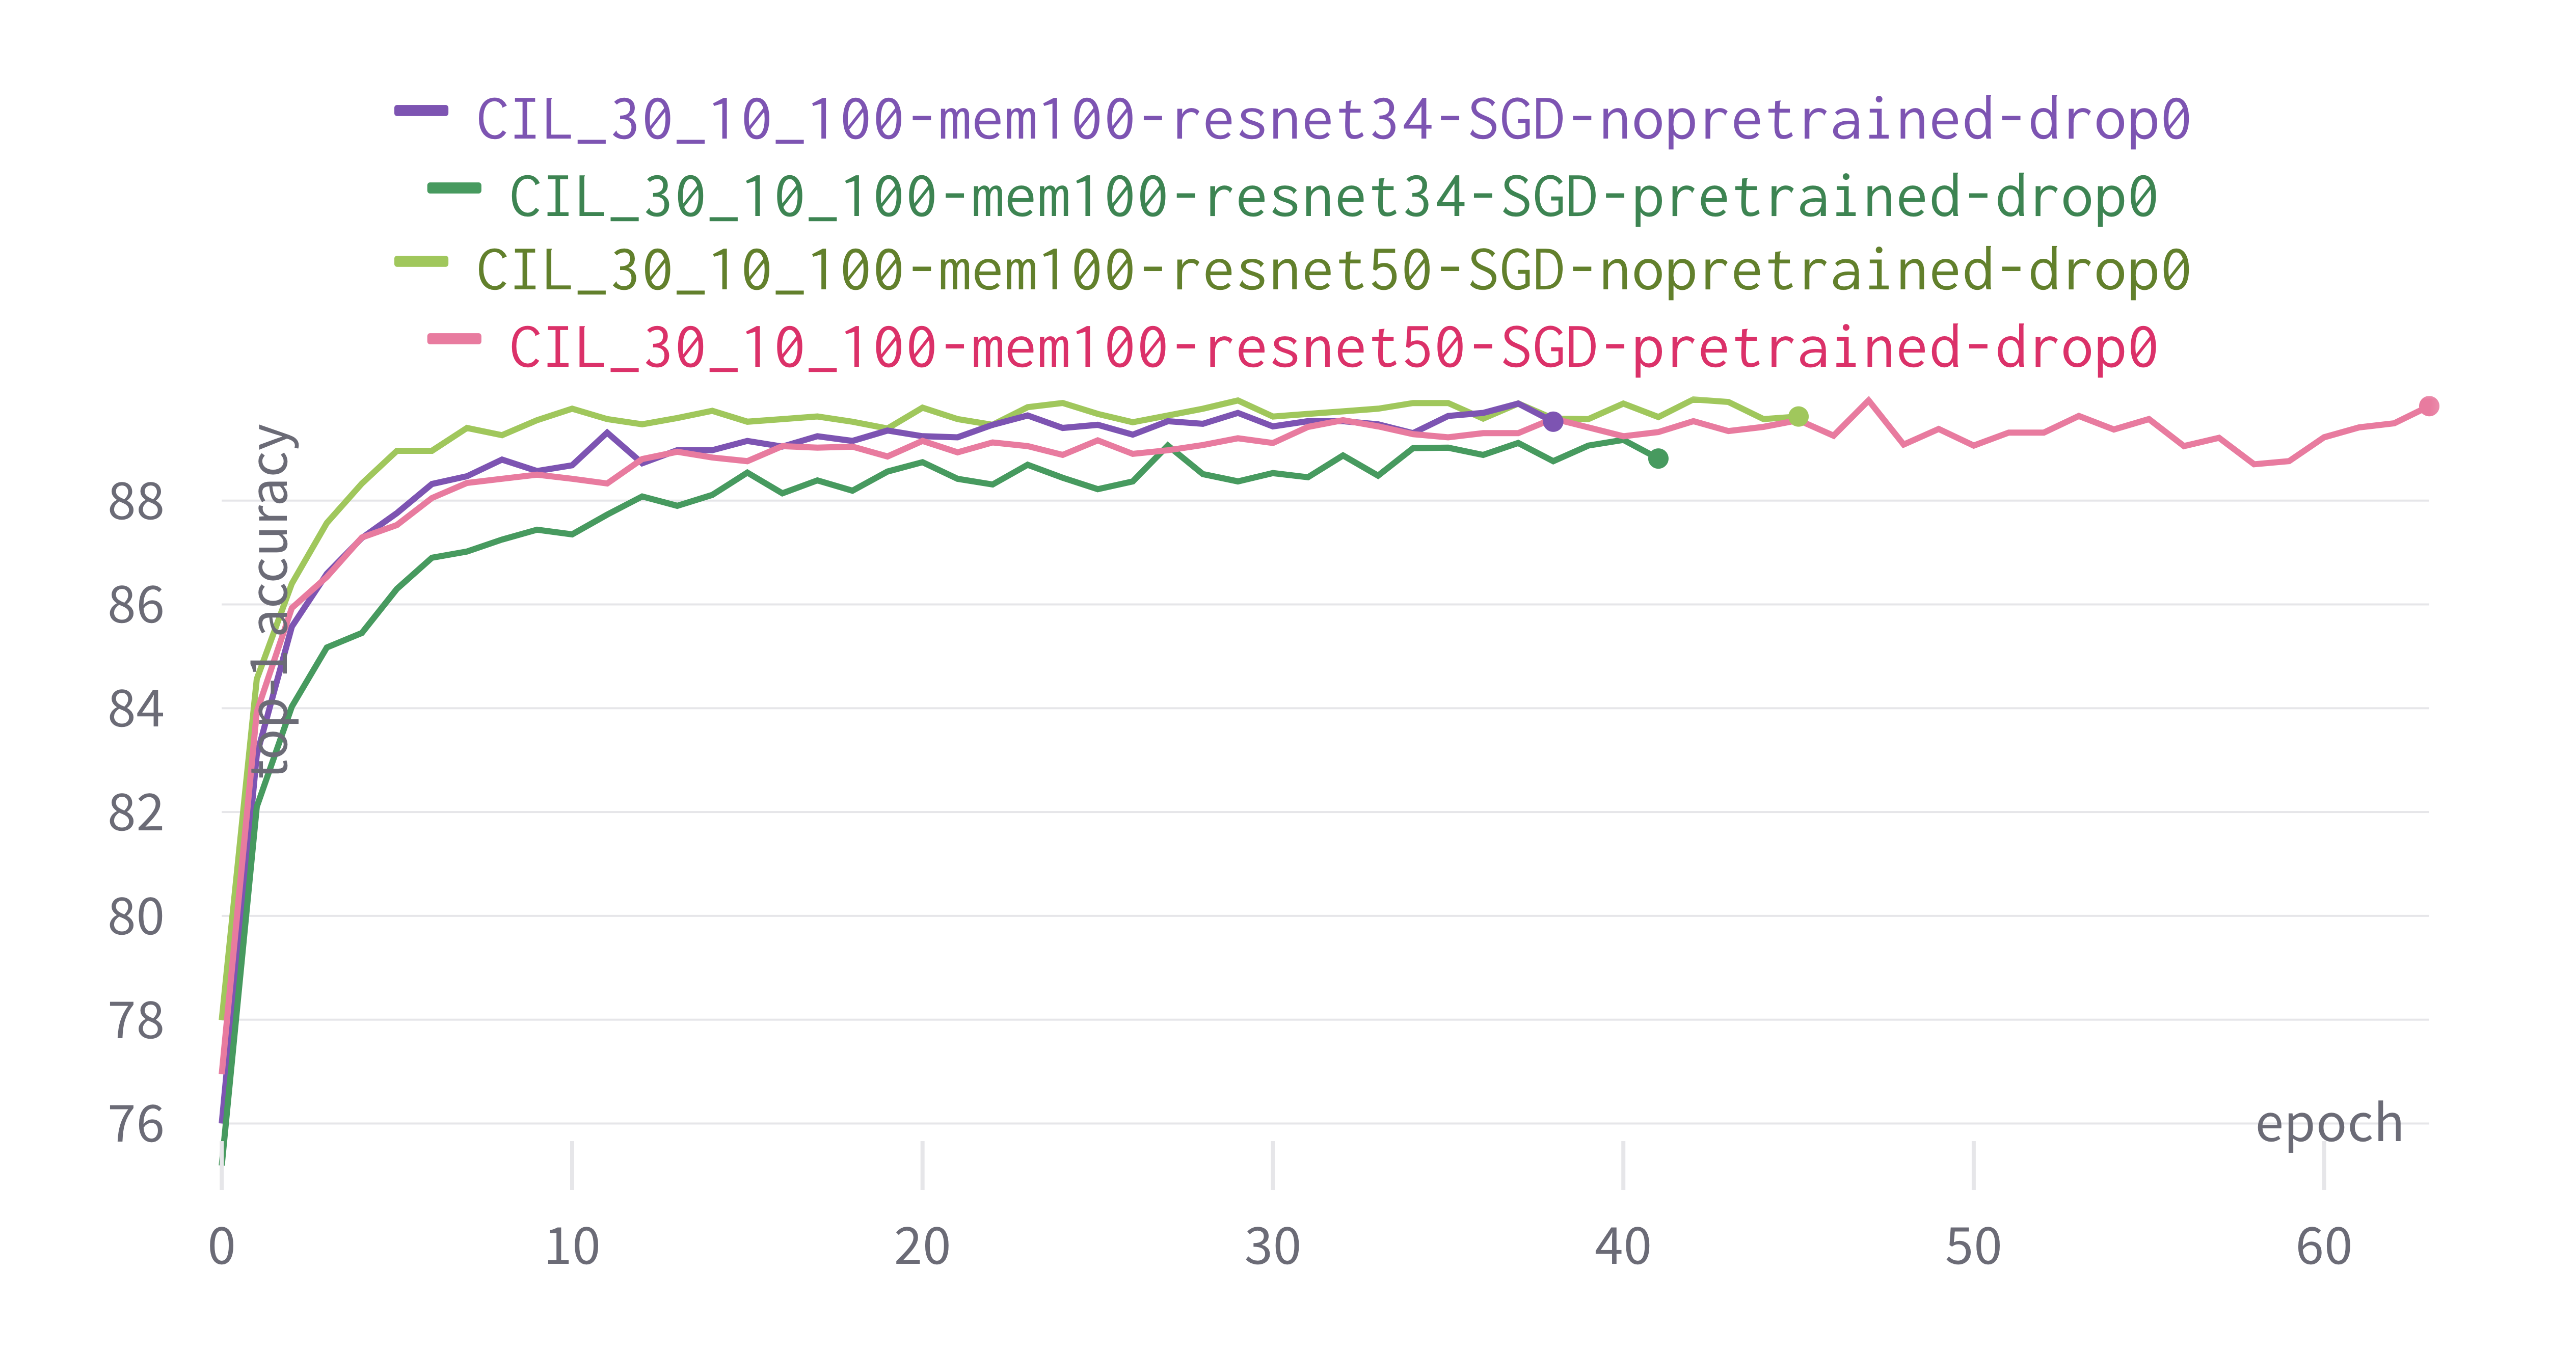
\includegraphics[width=0.50\textwidth]{images/exp/exp1-train.png} }}%
    %\qquad
    \centering
    \subfloat[\centering Accuracy on the validation set]{{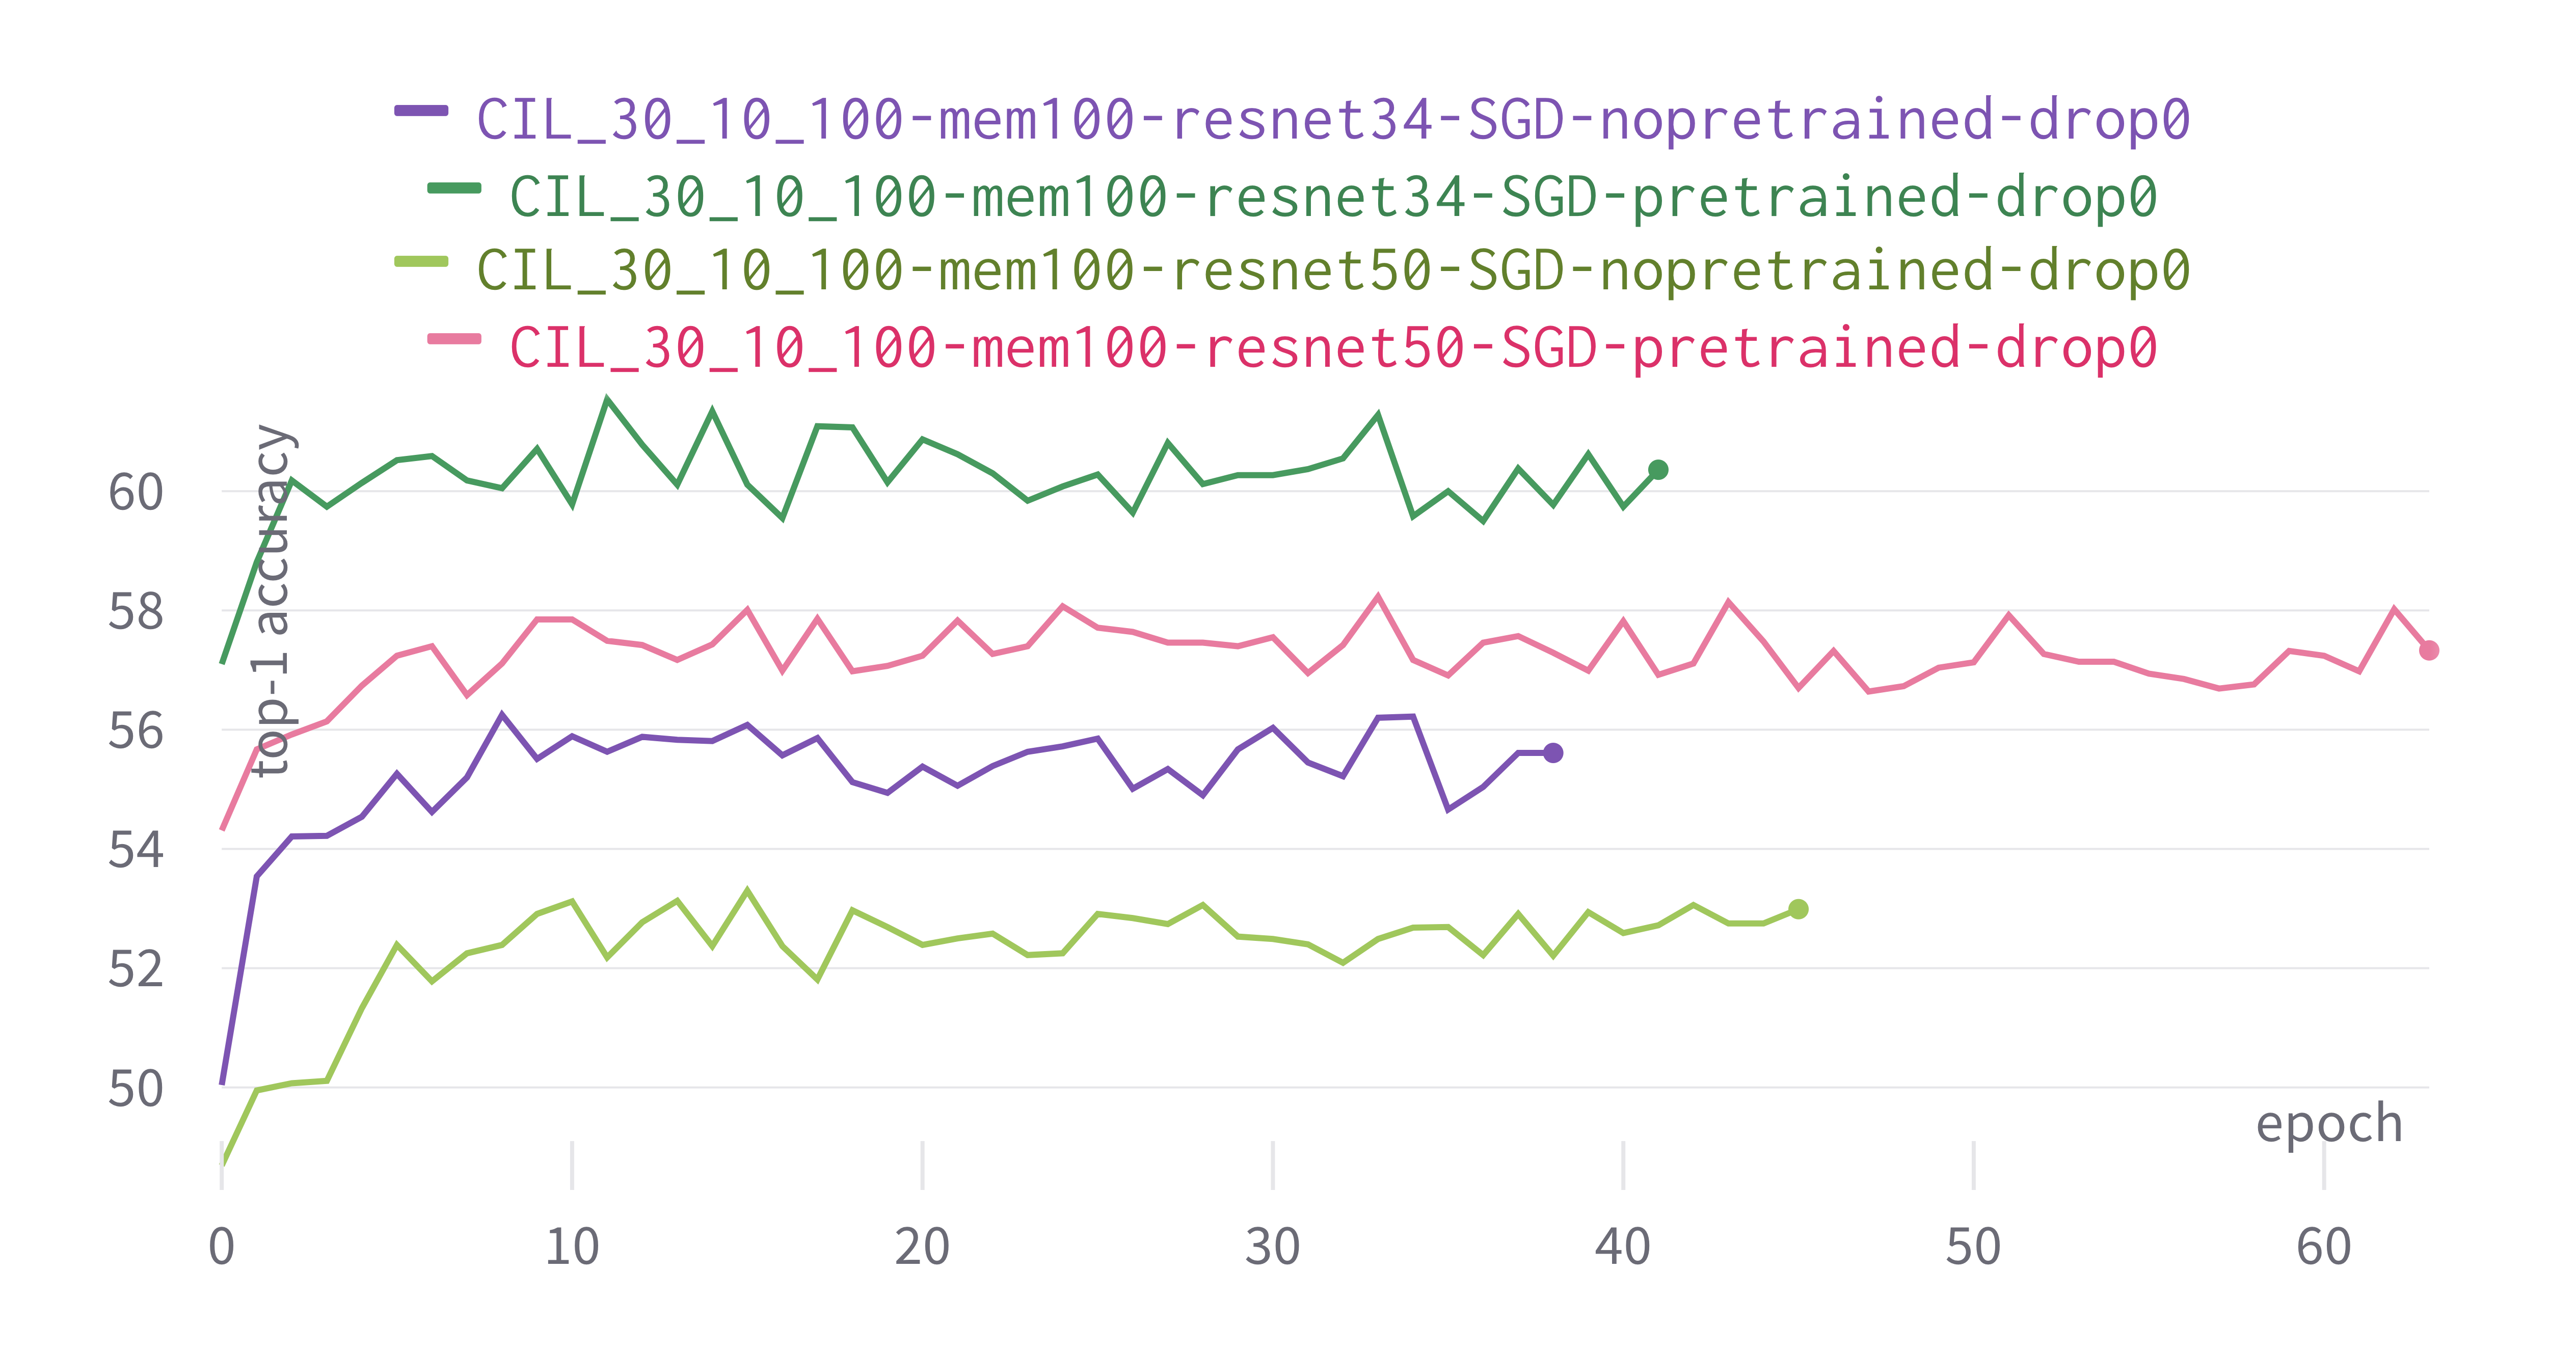
\includegraphics[width=0.50\textwidth]{images/exp/exp1-val.png} }}%
    \caption{Comparison of the accuracy of models at each training epoch. The images show the accuracy on training and validation sets at task 7.}%
    \label{fig:exp1-train_val}%
\end{figure}

\subsubsection{Regularization and data augmentation}
Following the analysis discussed above, it is necessary to regularize the model.
To do so, the next experiments are performed using the dropout layer (see \autoref{sec:methods-dropout}) and data augmentation (see \autoref{sec:methods-augment}). As said before, the backbone of each model is ResNet-34 pre-trained on ImageNet.

Using these techniques, performance is higher than before, as shown in \autoref{fig:exp2}.
From \autoref{fig:exp2-train_val} we can see that the training accuracy of the models with regularization is lower than that of models without regularization, but the validation accuracy is higher.
This is a sign that regularization works as expected.

As shown in \autoref{table:exp2}, the top-1 accuracy of the best regularized model adopting data augmentation is 7\% higher than that without regularization and data augmentation.


%\newpage
\begin{figure}[H]
	\centering
	\subfloat[\centering Top-1 accuracy]{{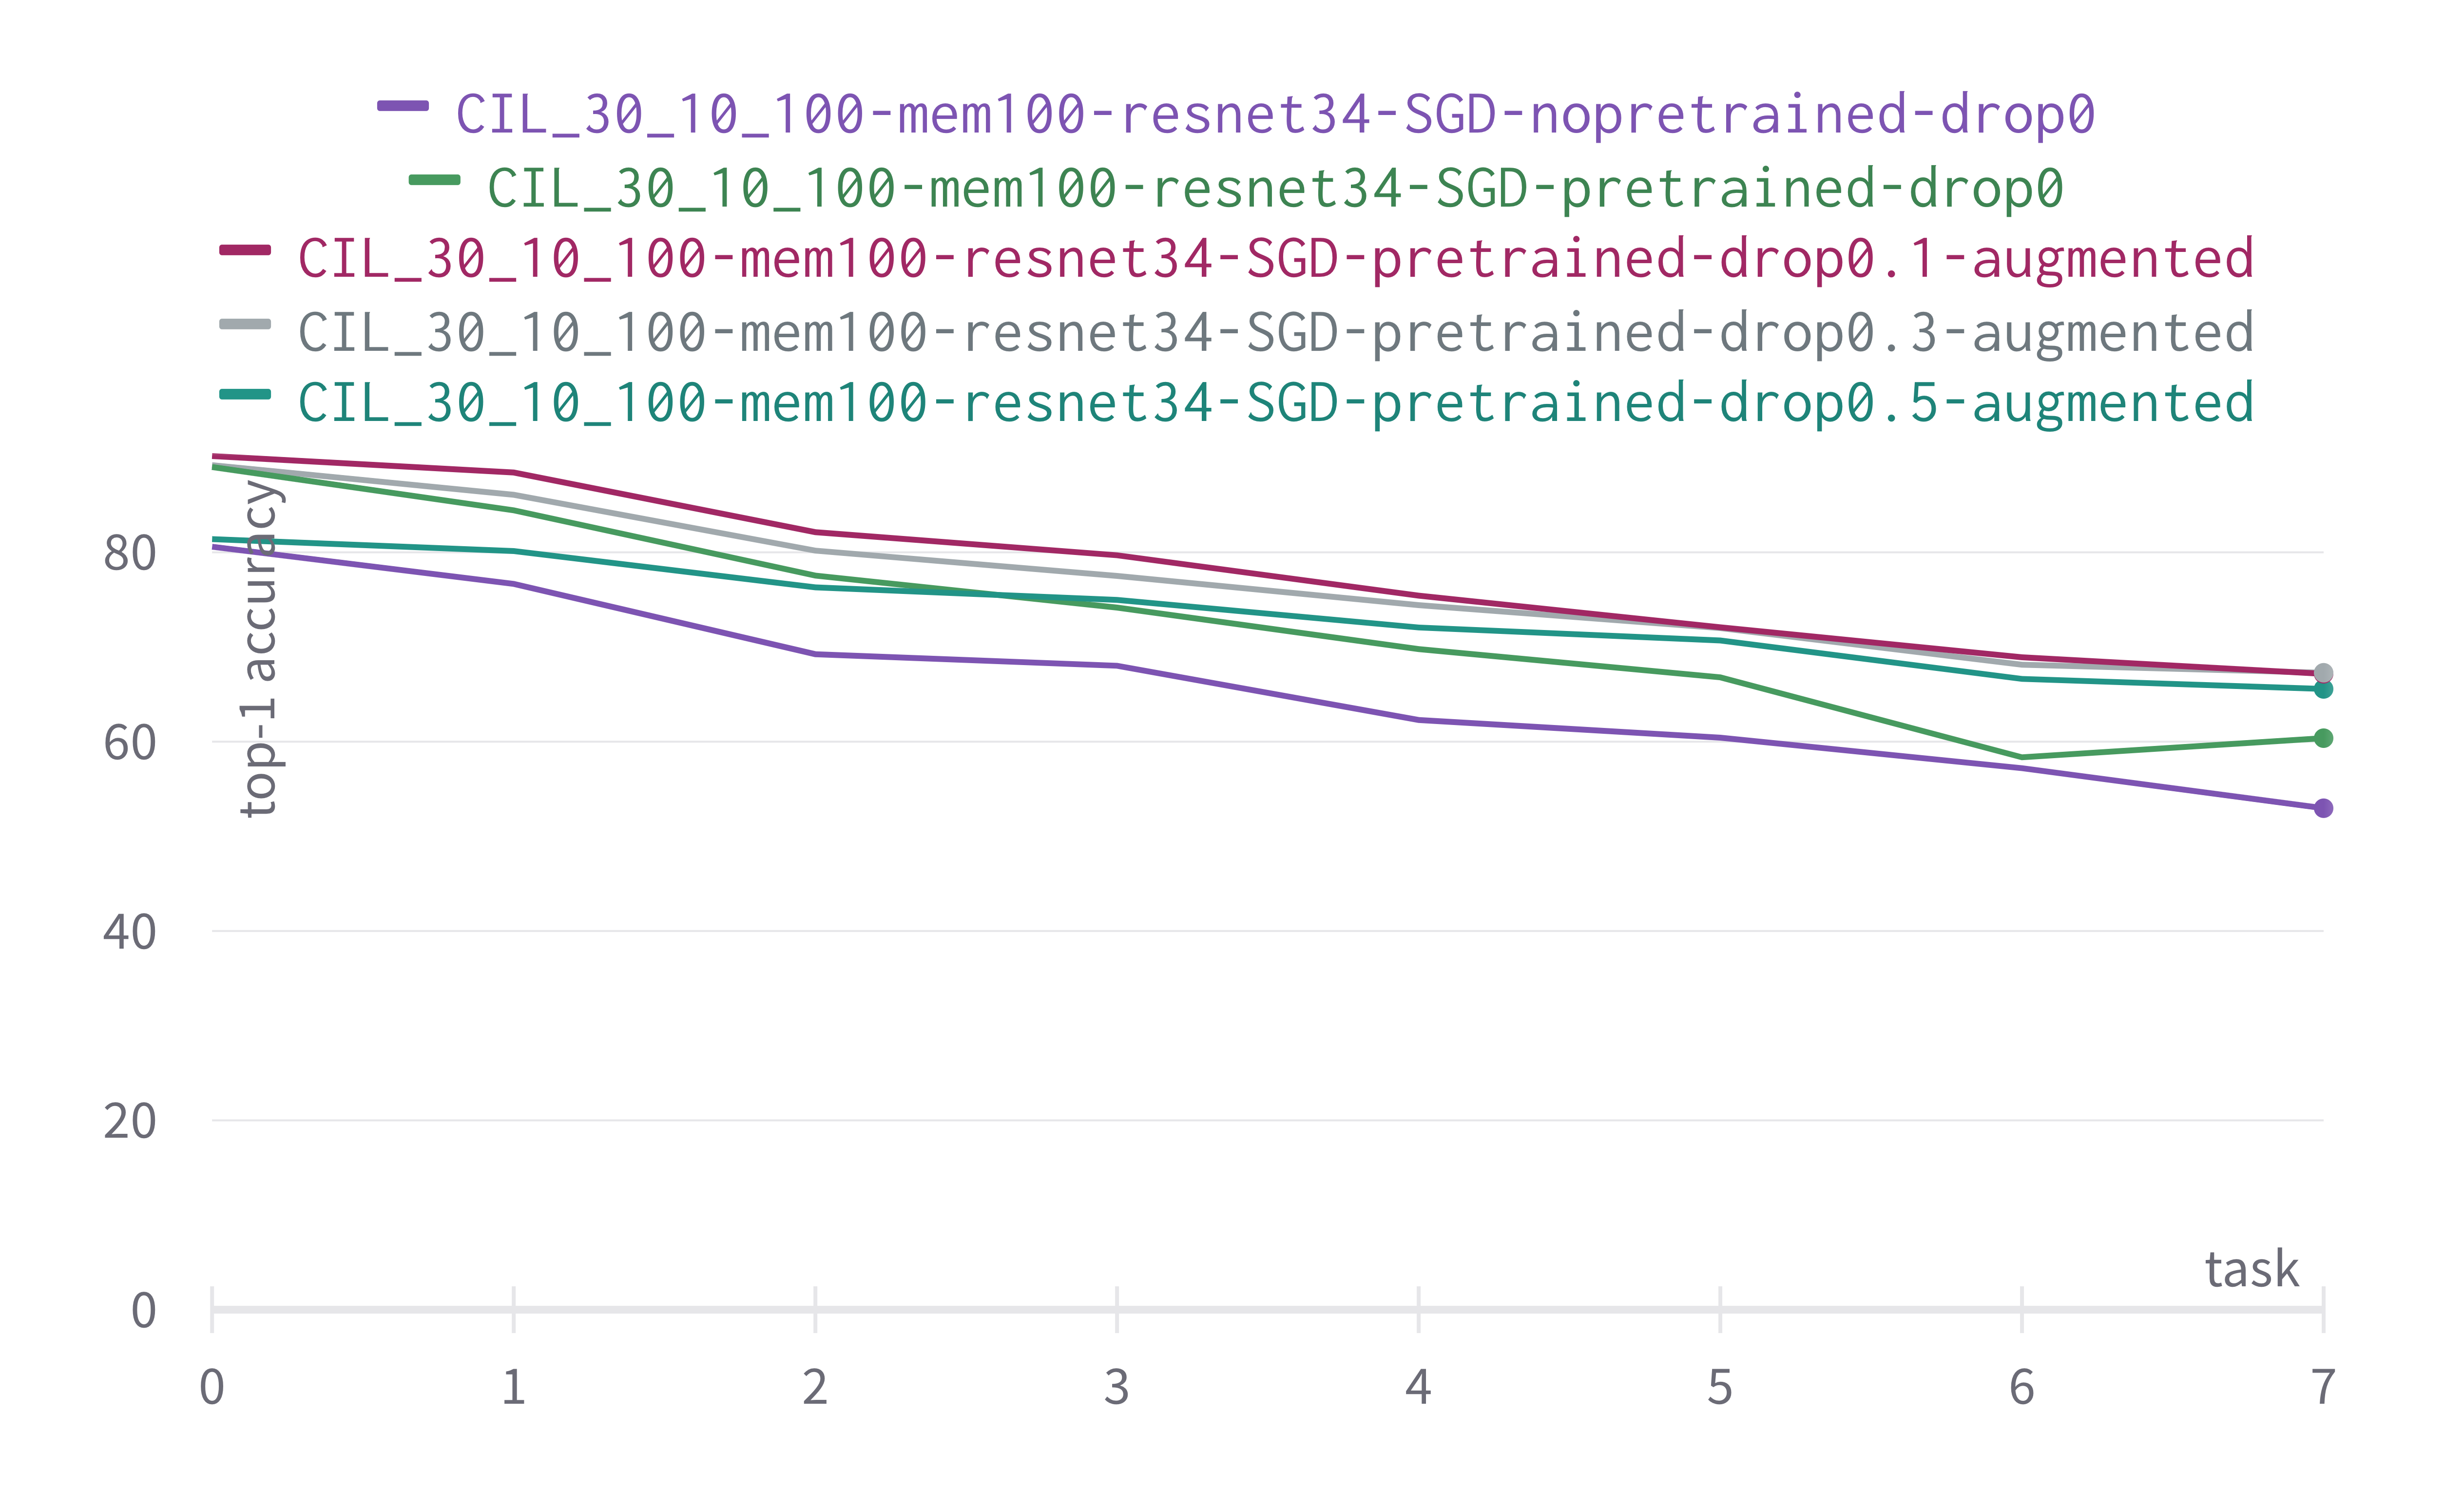
\includegraphics[width=0.50\textwidth]{images/exp/exp2-top1.png} }}%
    %\qquad
	\subfloat[\centering Top-5 accuracy]{{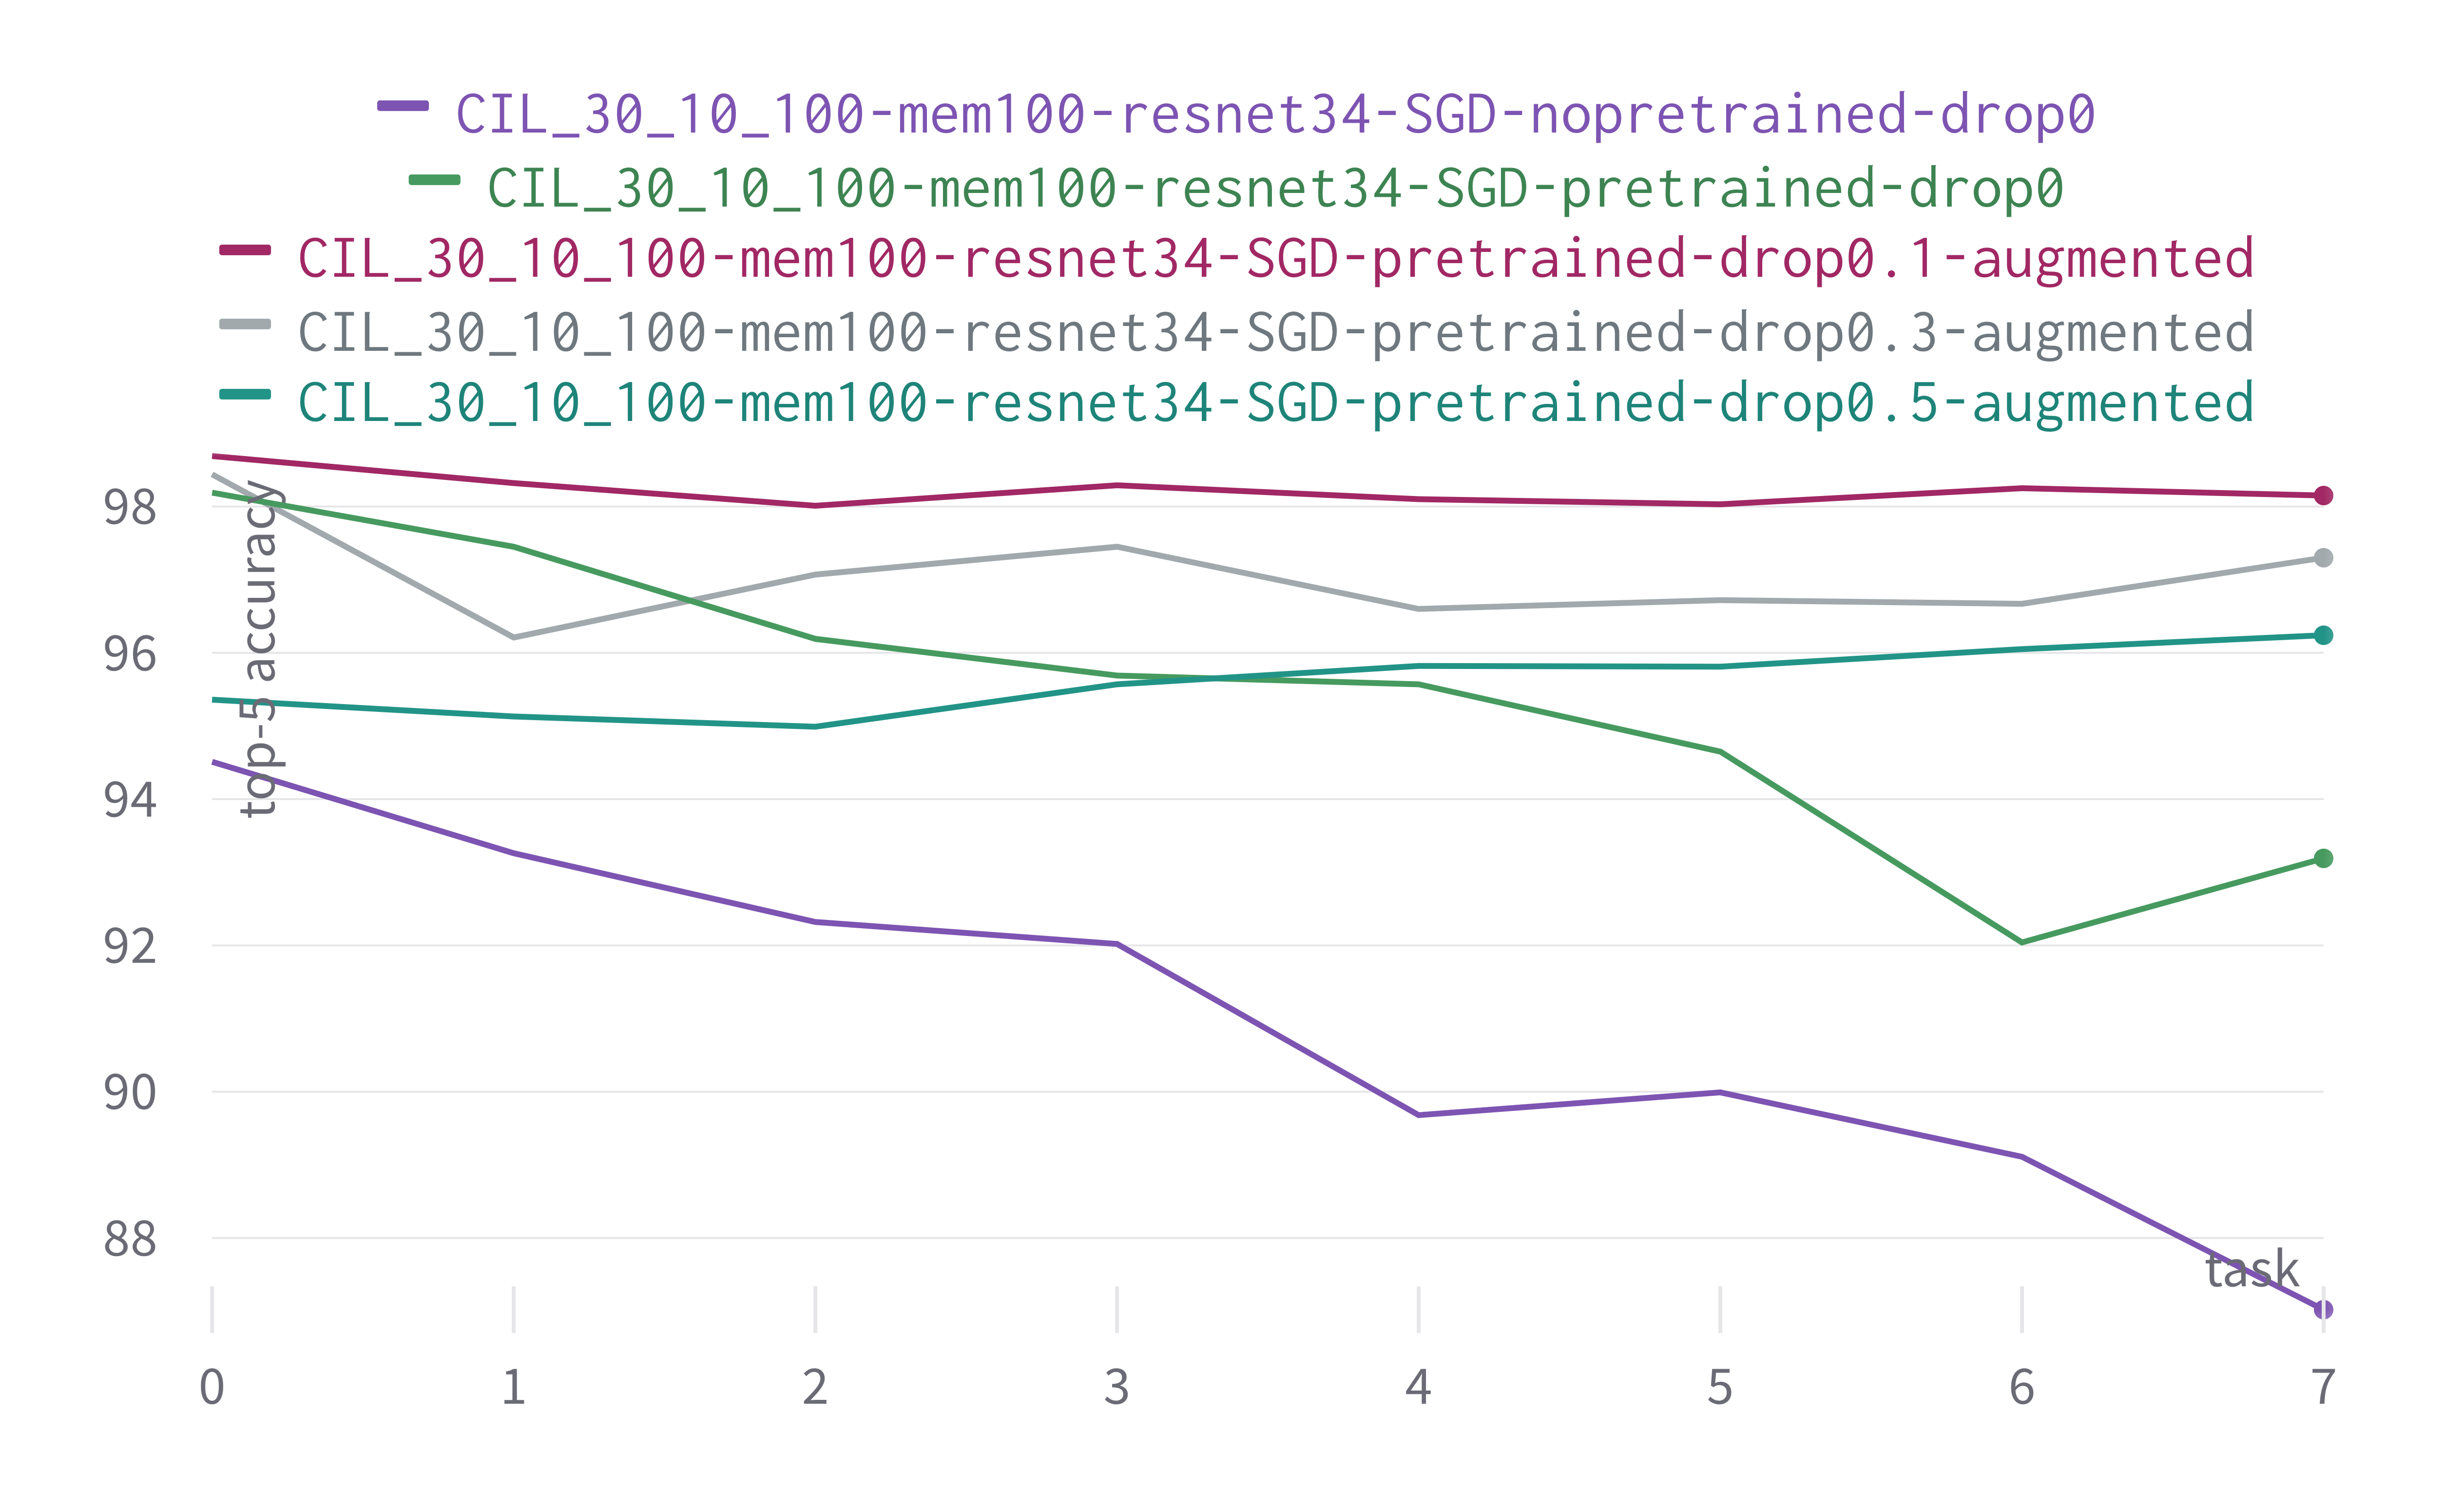
\includegraphics[width=0.50\textwidth]{images/exp/exp2-top5.png} }}%
	\caption{Top-1 and top-5 accuracy of the regularized models using data augmentation at different CIL tasks.}%
	\label{fig:exp2}%
\end{figure}

\begin{table}[H]
    \centering
    \centerline{
    \begin{tabular}{c|c|c|c|c}
        \hline
        \textbf{Model} &
        \textbf{Data} &
        \textbf{Dropout} &
        \textbf{Top-1} & 
        \textbf{Top-5} \\
        \textbf{name} &
        \textbf{augm.} &
        \textbf{rate} &
        \textbf{acc. (\%)} & 
        \textbf{acc. (\%)} \\
        \hline
        \hline
SGD-nopretrained-drop0 &no&0.0& 52.97 & 87.02\\
SGD-pretrained-drop0 &no&0.0& 60.37 & 93.19\\
\hline
SGD-pretrained-drop0.1-augmented&yes&0.1&	67.17&\textbf{98.15}\\
SGD-pretrained-drop0.3-augmented&yes&0.3&\textbf{67.28}&	97.3\\
SGD-pretrained-drop0.5-augmented&yes&0.5&65.57&	96.24\\
        \hline        
    \end{tabular}}
    \caption{Regularized models with data augmentation. Top-1 and top-5 accuracy at task 7.}
    \label{table:exp2}
\end{table}

\begin{figure}[H]
	\centering
	\subfloat[\centering Accuracy on the training set]{{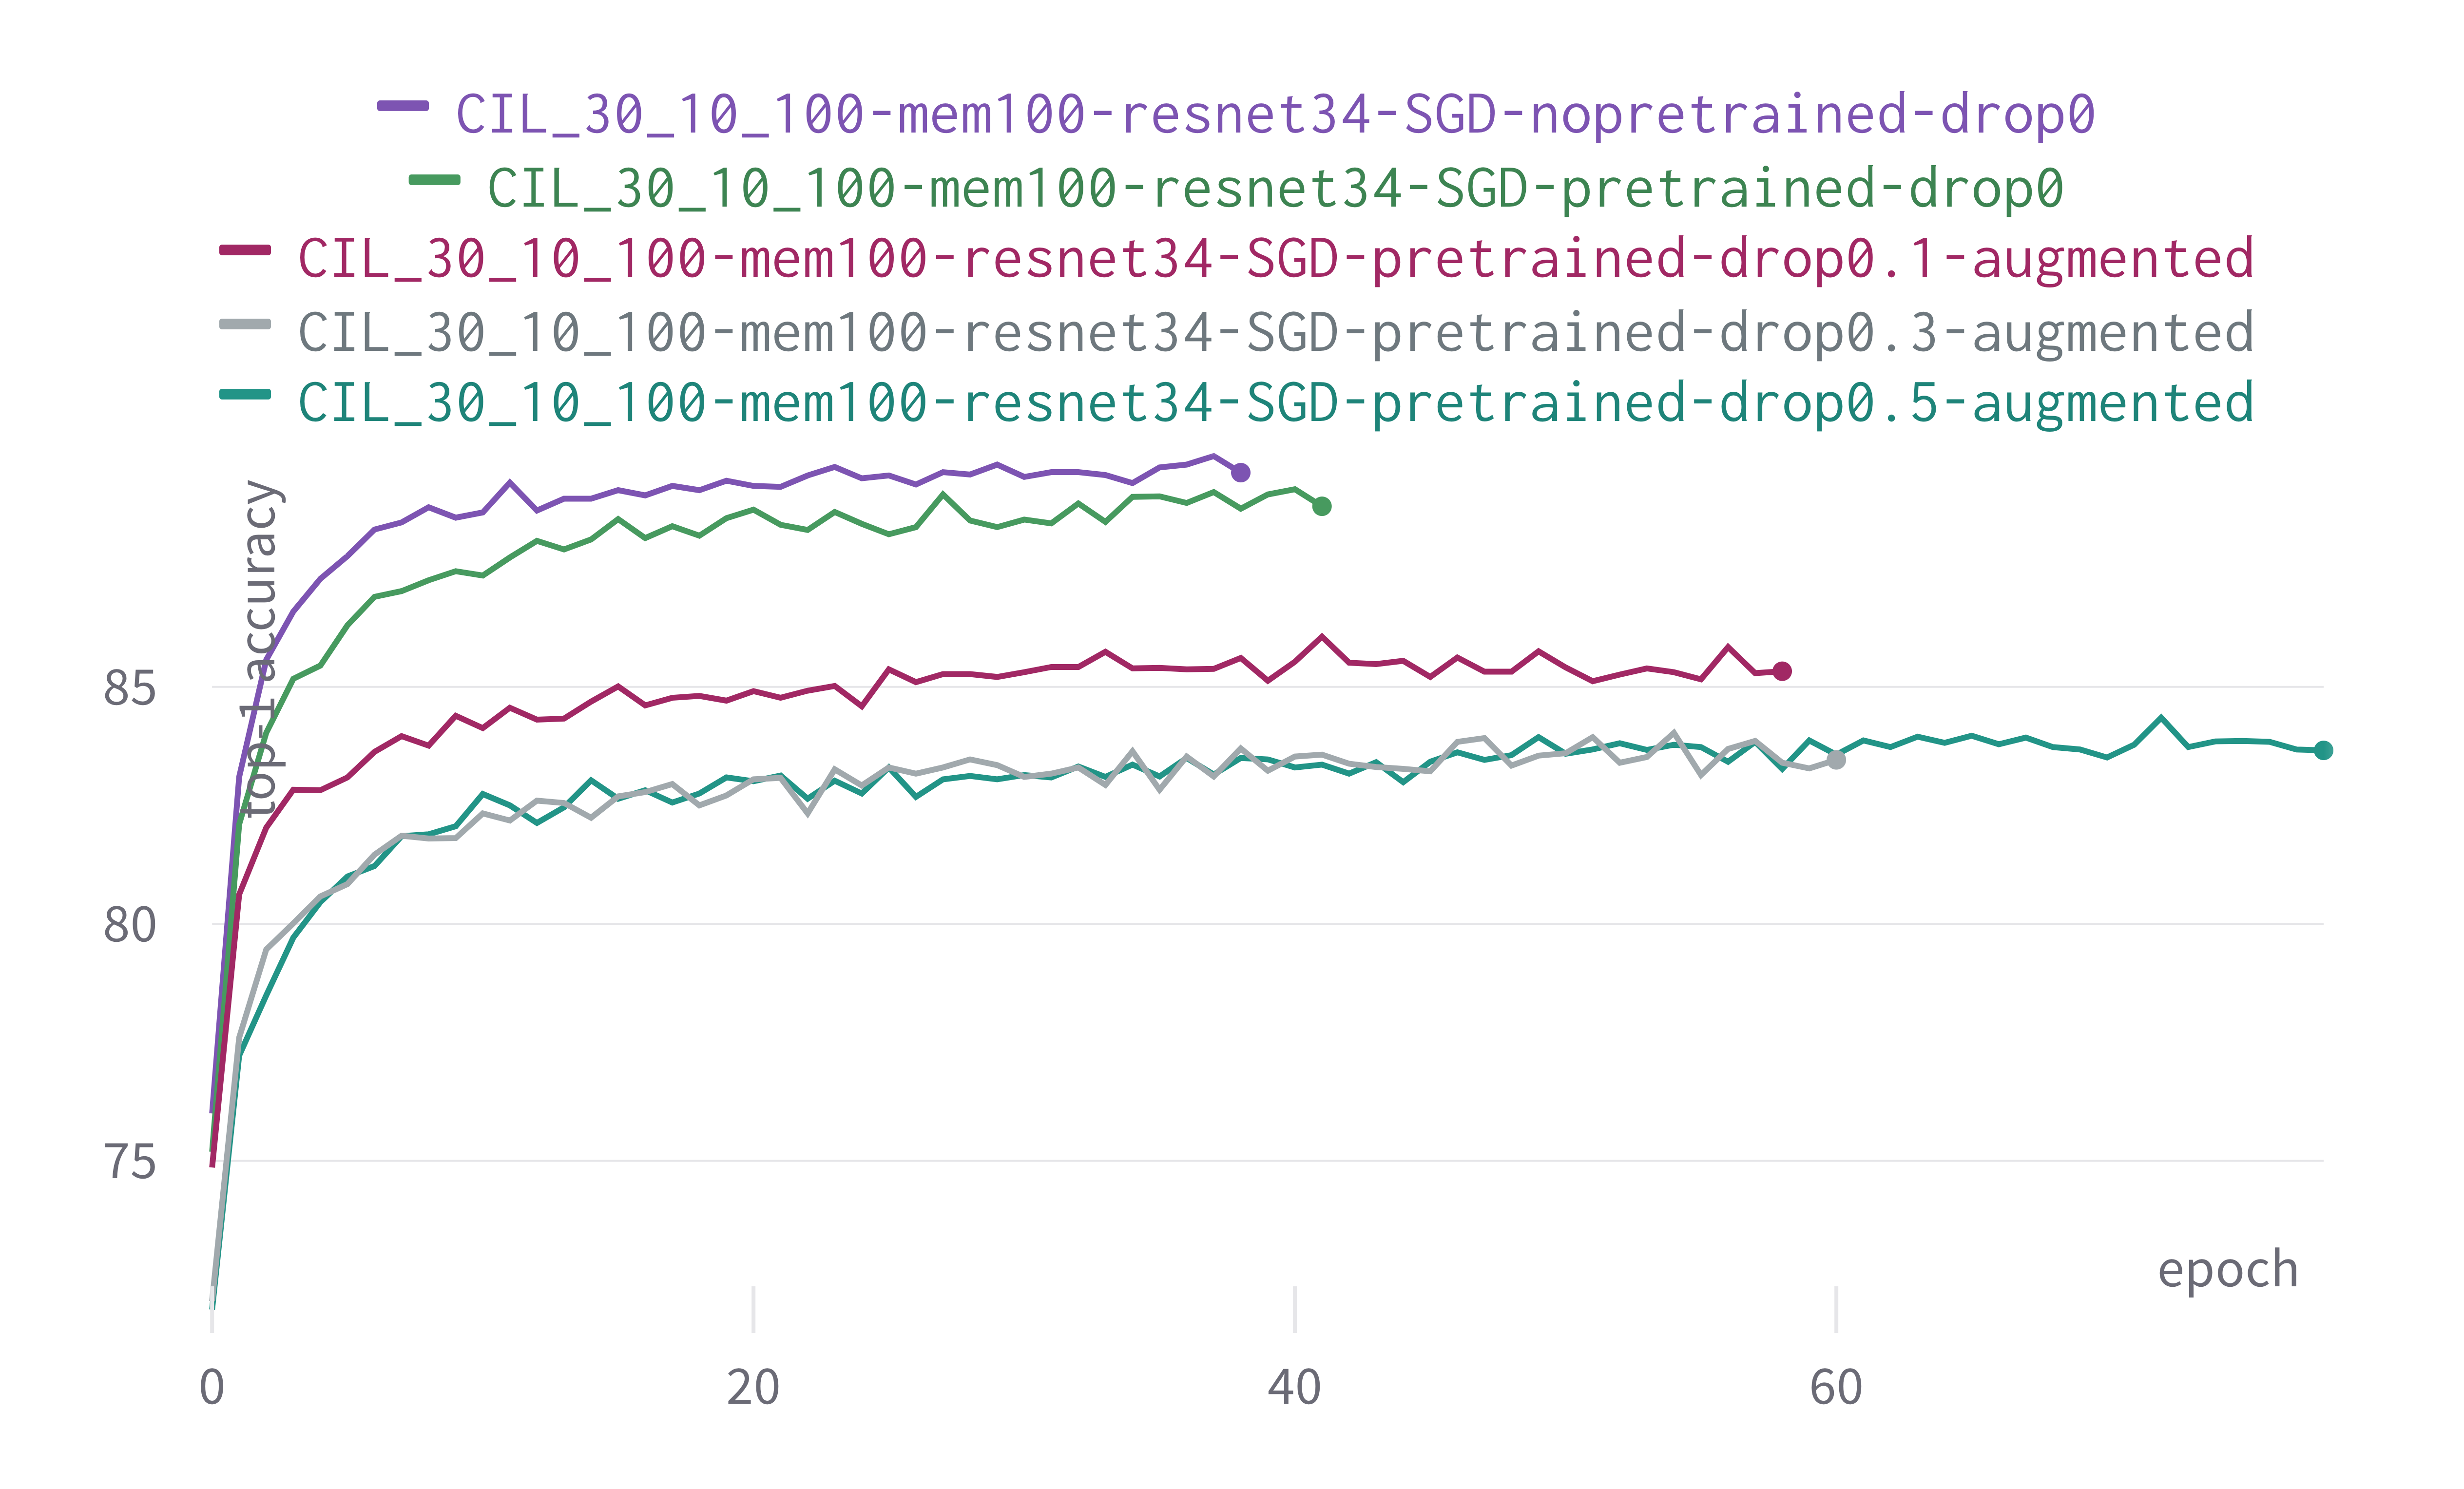
\includegraphics[width=0.50\textwidth]{images/exp/exp2-train.png} }}%
    %\qquad
	\subfloat[\centering Accuracy on the validation set]{{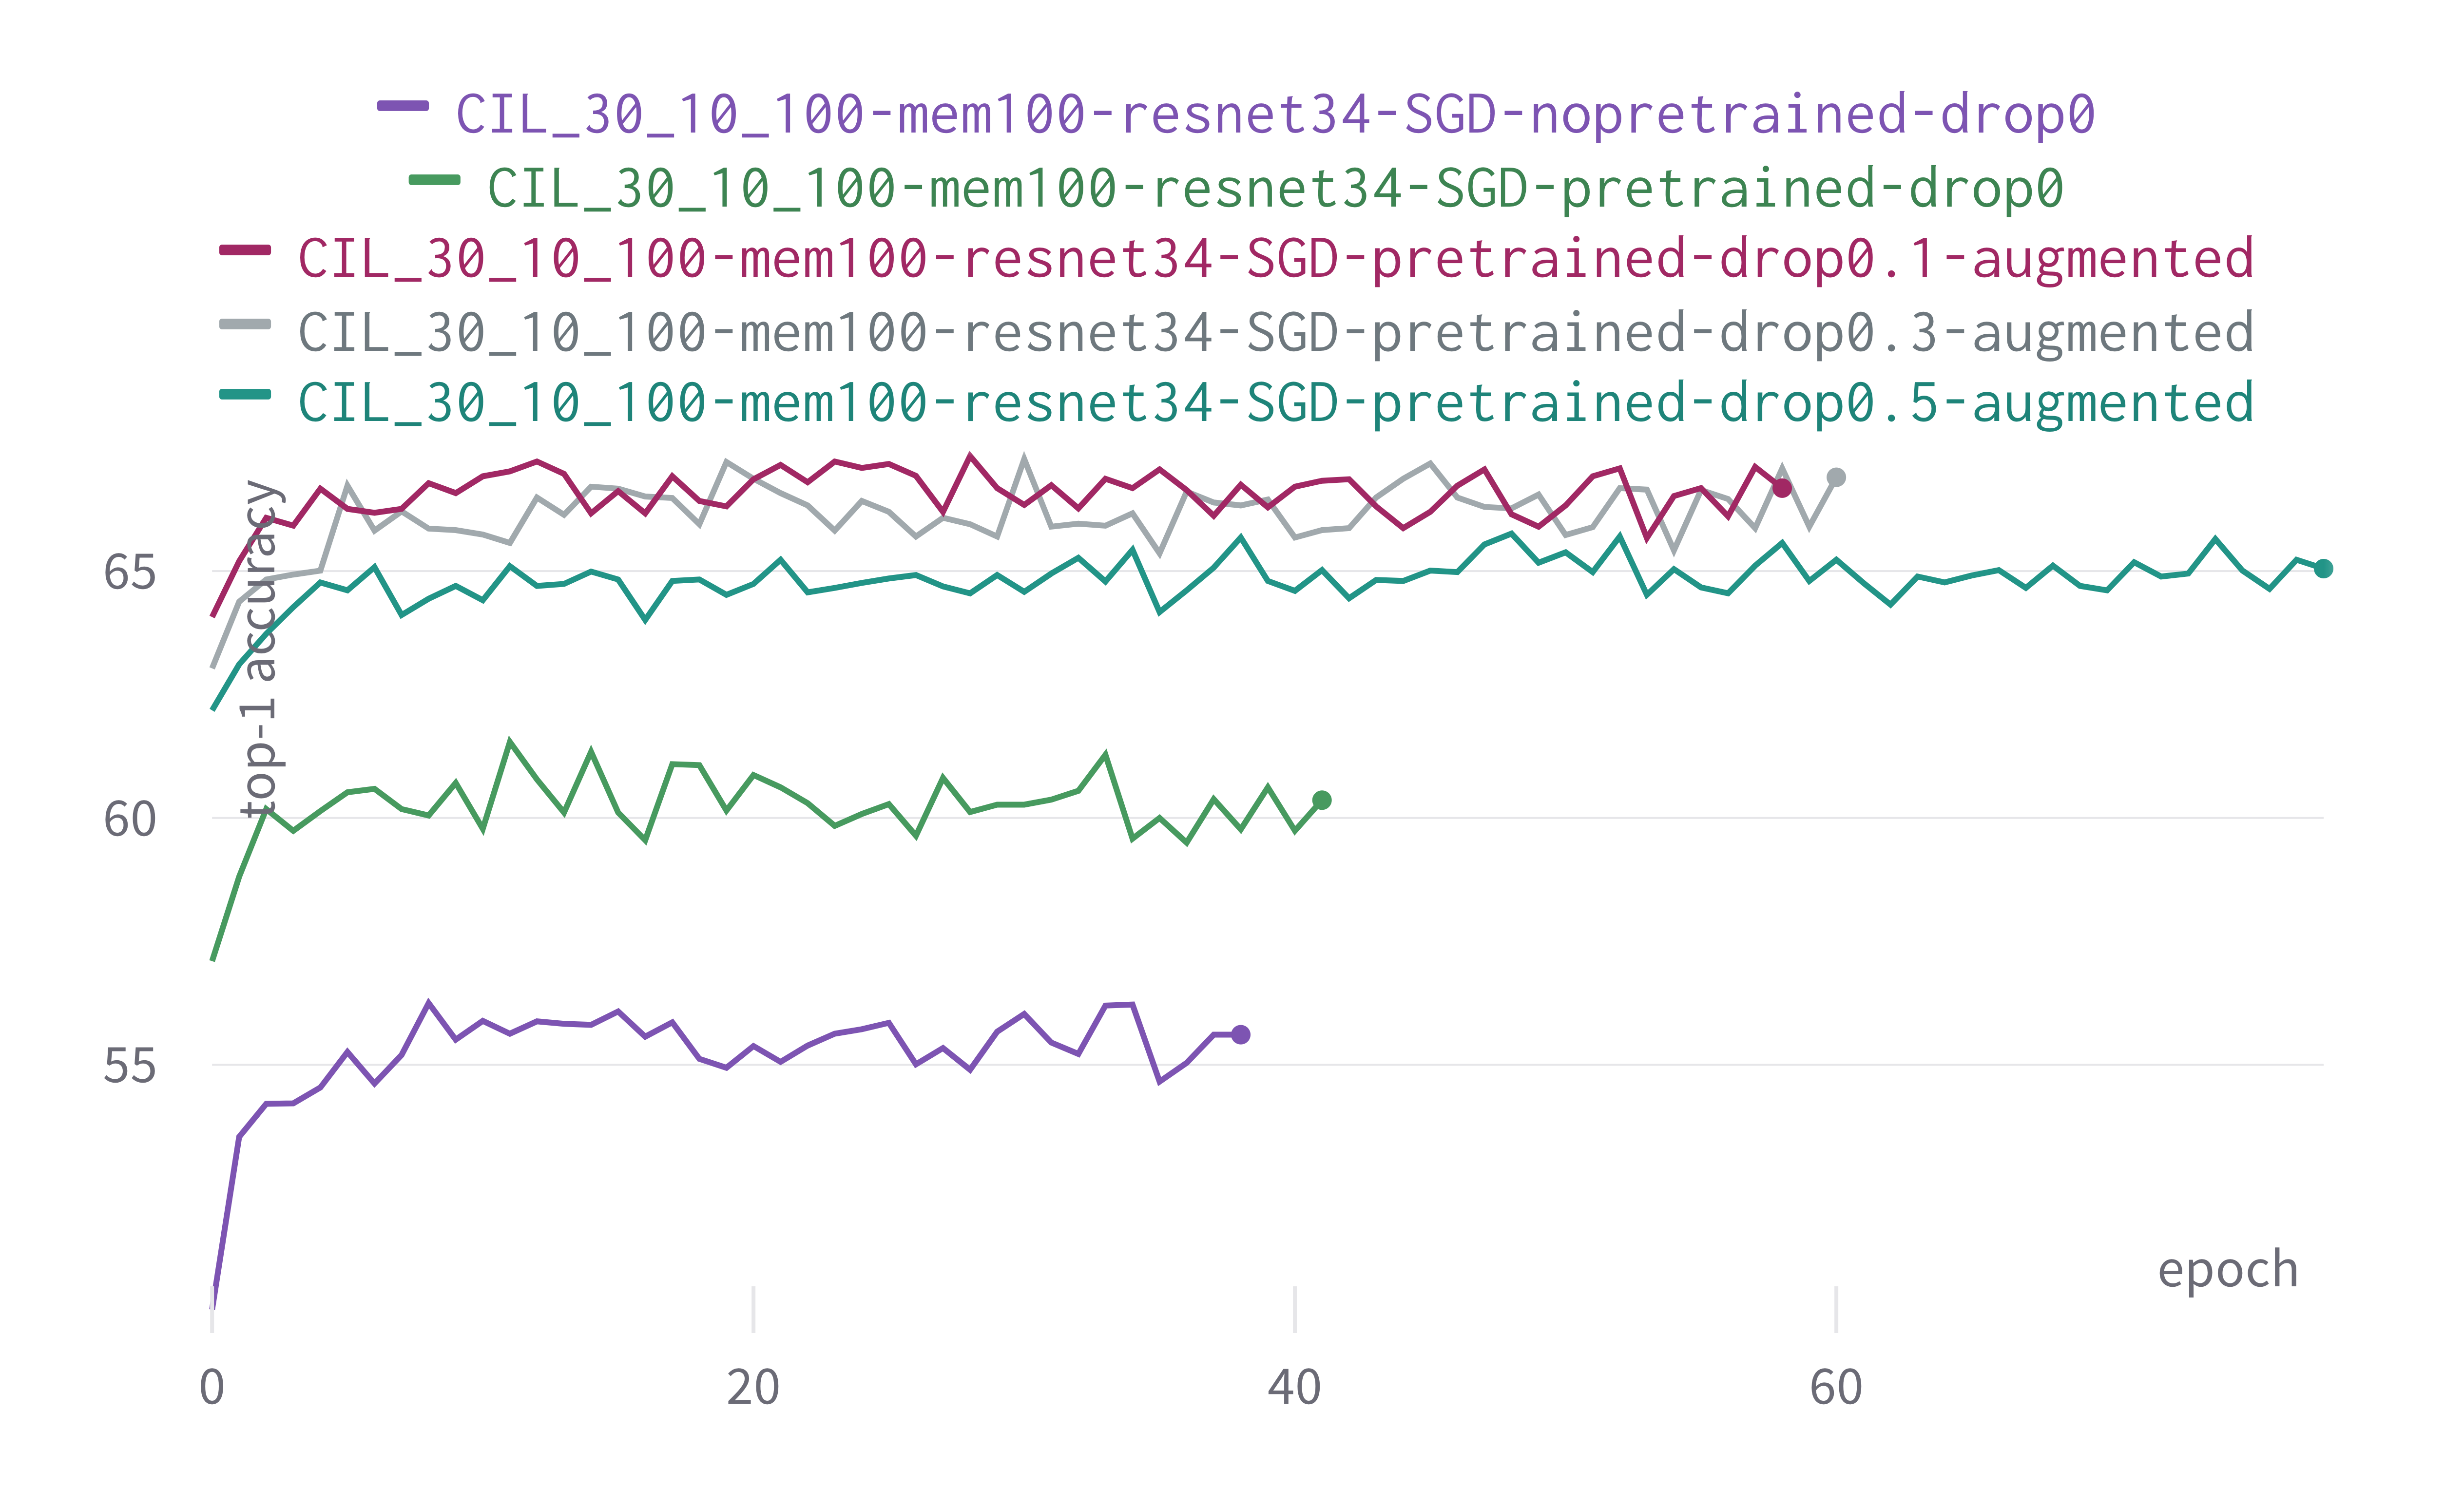
\includegraphics[width=0.50\textwidth]{images/exp/exp2-val.png} }}%
	\caption{Regularized models with data augmentation. The images show the training history of models at task 7, comparing the top-1 accuracy at each training epoch calculated on the training and validation set.}
	\label{fig:exp2-train_val}%
\end{figure}

%\newpage
\subsubsection{Type 1 baseline}
To compare the performance of the CIL model with a standard non-incremental learning setup, a baseline is trained using the same training, validation and test sets as the CIL model.
Specifically, these experiments exploit the type 1 baseline definition described in \autoref{sec:method-baseline1}, i.e. the baseline uses the DER algorithm and trains the model at task 0 with all 100 classes.
As with the CIL model, the baseline uses: data augmentation, the SGD optimizer, a dropout layer before the FC layer, ResNet-34 pre-trained on ImageNet as the backbone for feature extraction.

Performance comparison between CIL models and baselines considers the top-1 accuracy on the test set, results are shown in \autoref{table:baseline1}.
As we can see, the best CIL model performs better than the best baseline, which is the opposite of what is expected.
However, as shown in \autoref{table:baseline1-params}, this is due to the difference in the number of model parameters described in \autoref{sec:method-baseline1}.
For this reason, to achieve a more reliable comparison, a new baseline will be used later on.

\begin{table}[H]
    \centering
    \centerline{
    \begin{tabular}{c|c|c}
        \hline
        \textbf{Model} &
        \textbf{Dropout} &
        \textbf{Top-1}\\
        \textbf{name} &
        \textbf{rate} &
        \textbf{acc. (\%)} \\
        \hline
\hline
SGD-pretrained-drop0.1-augmented&0.1&67.17\\
SGD-pretrained-drop0.3-augmented&0.3&\textbf{67.28}\\
SGD-pretrained-drop0.5-augmented&0.5&65.57\\
\hline
BASELINE\_1-pretrained-drop0.1-augmented&0.1&63.04\\
BASELINE\_1-pretrained-drop0.3-augmented&0.3&61.15\\
BASELINE\_1-pretrained-drop0.5-augmented&0.5&57.14\\
\hline 
    \end{tabular}}
    \caption{Performance comparison between CIL models and type 1 baselines. Top-1 accuracy at task 7 and task 0 respectively.}
    \label{table:baseline1}
\end{table}

\begin{table}[H]
    \centering
    \centerline{
    \begin{tabular}{c|c}
        \hline
        \textbf{Model} &
        \textbf{\#Params} \\
        \textbf{name} &
        \textbf{(M)} \\
        \hline
\hline
SGD-pretrained-drop0.1-augmented&170\\
SGD-pretrained-drop0.3-augmented&170\\
SGD-pretrained-drop0.5-augmented&170\\
\hline
BASELINE\_1-pretrained-drop0.1-augmented&21\\
BASELINE\_1-pretrained-drop0.3-augmented&21\\
BASELINE\_1-pretrained-drop0.5-augmented&21\\
\hline 
    \end{tabular}}
    \caption{Number of parameters of CIL models and the type 1 baselines at task 7 and task 0 respectively.}
    \label{table:baseline1-params}
\end{table}

\subsubsection{Top-100 Classes}
\label{sec:cil-top100}
In order to assess the extent to which classes with few examples contribute to the deterioration in performance, the following experiments consider only the top-100 classes, i.e. those classes with the most examples (see the left-hand side of the distribution in \autoref{fig:logodet-dist}).
This is useful to be aware of how much the model is limited in performance by the dataset.

Using regularization and data augmentation, models trained on 100 randomly sampled classes and those trained on the top-100 classes are compared in \autoref{fig:exp3} and \autoref{table:exp3}.
As we can see, although the top-5 accuracy does not change, considering the top-1 accuracy we can see a drastic improvement in performance.
This indicates that classes with few examples significantly deteriorate performance.

\begin{figure}[H]
	\centering
	\subfloat[\centering Top-1 accuracy]{{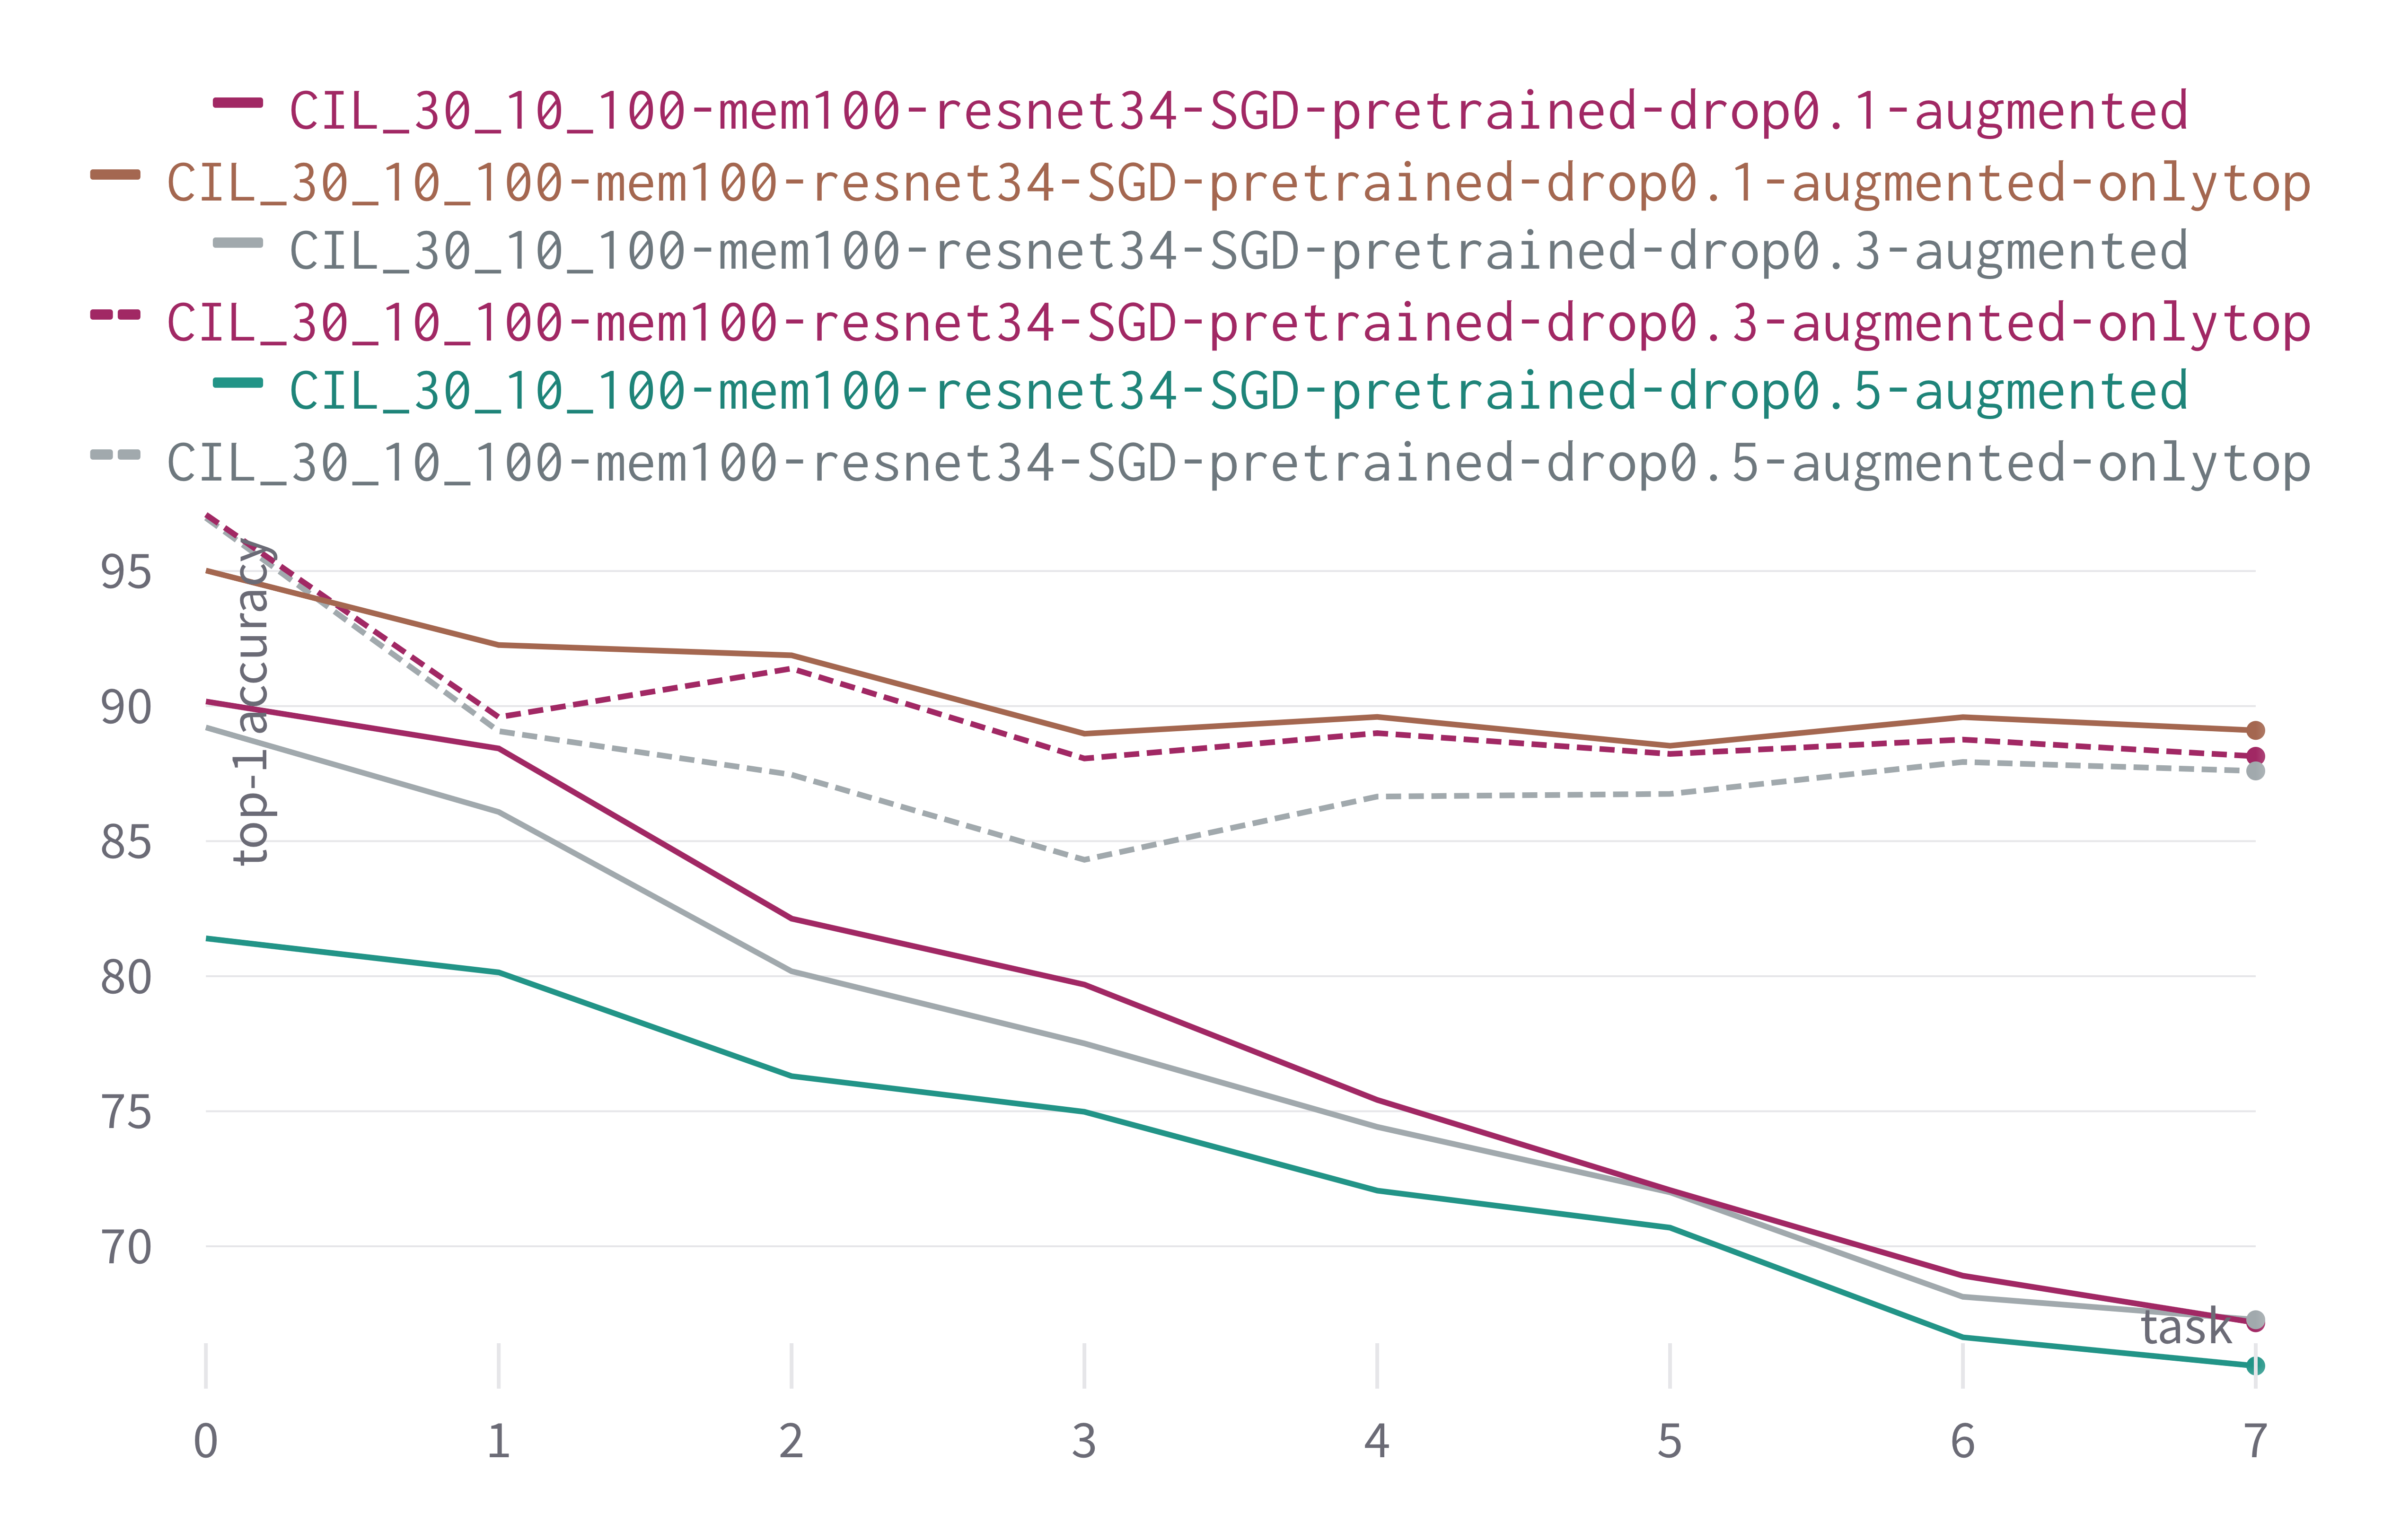
\includegraphics[width=0.50\textwidth]{images/exp/exp3-top1.png} }}%
    %\qquad
	\subfloat[\centering Top-5 accuracy]{{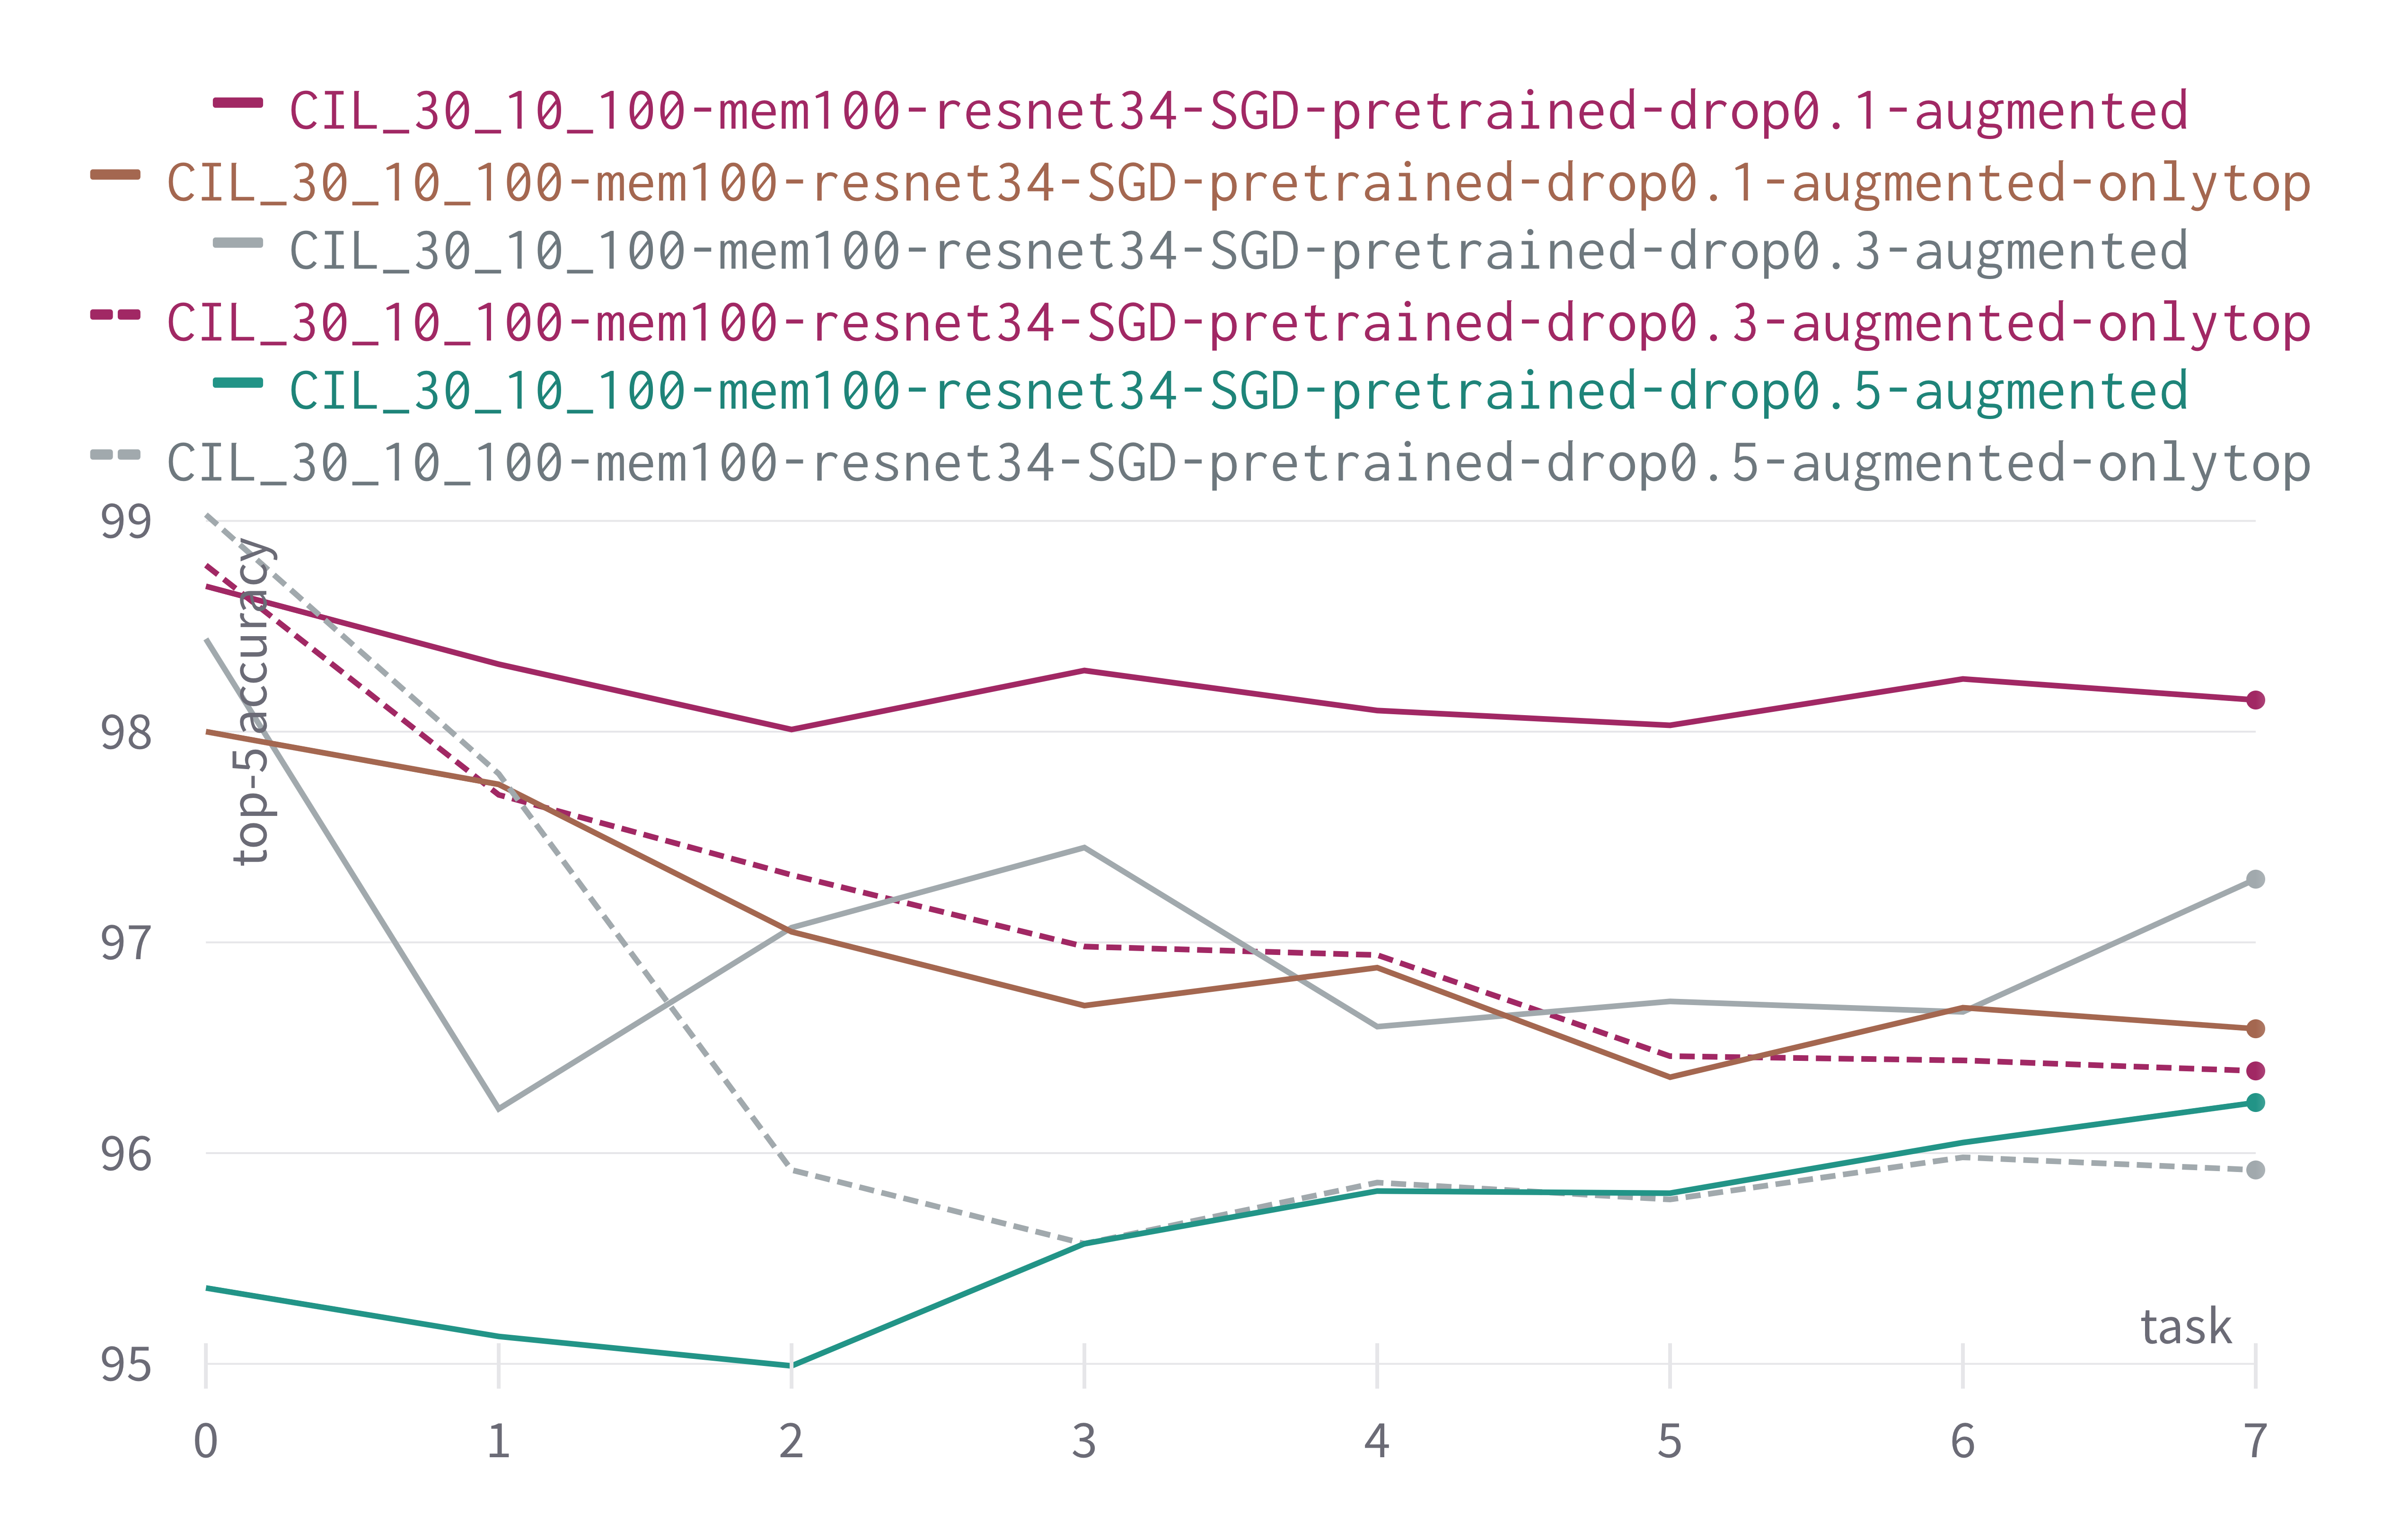
\includegraphics[width=0.50\textwidth]{images/exp/exp3-top5.png} }}%
	\caption{Comparison between models trained on 100 randomly sampled classes and those trained on the top-100 classes considering top-1 and top-5 at each task.}%
	\label{fig:exp3}%
\end{figure}

\begin{table}[H]
    \centering
    \centerline{
    \begin{tabular}{c|c|c|c|c}
        \hline
        \textbf{Model} &
        \textbf{Dropout} &
        \textbf{Sampling} &
        \textbf{Top-1} & 
        \textbf{Top-5} \\
        \textbf{name} &
        \textbf{rate} &
        \textbf{method} &
        \textbf{acc. (\%)} & 
        \textbf{acc. (\%)} \\
        \hline
        \hline
drop0.1-augmented&0.1&random&	67.17&98.15\\
drop0.3-augmented&0.3&random&67.28&	97.3\\
drop0.5-augmented&0.5&random&65.57&	96.24\\
\hline
drop0.1-augmented-onlytop&0.1&top-100&\textbf{89.1}&\textbf{96.59}\\
drop0.3-augmented-onlytop&0.3&top-100&88.14&96.39\\
drop0.5-augmented-onlytop&0.5&top-100&87.6&95.92\\
        \hline
    \end{tabular}}
    \caption{Comparison between models trained on 100 randomly sampled classes and those trained on the top-100 classes. Top-1 and top-5 accuracy at task 7.}
    \label{table:exp3}
\end{table}
%\newpage

%\newpage
\subsubsection{Introduction of Adam optimizer}
The next experiments aim to compare SGD (see \autoref{sec:sgd_opt}) and Adam (see \autoref{sec:adam_opt}) optimizers.
Using regularization, data augmentation and the top-100 classes, the results of this comparison are, shown in \autoref{fig:exp4} and \autoref{table:exp4}.

As we can see, the top-1 accuracy at task 7 improves by more than 6\% using Adam as optimization algorithm. 
In addition to the performance aspect, the training history in \autoref{fig:exp4-train_val} shows that Adam leads to faster convergence. In fact, models trained with this algorithm achieve the highest value of top-1 accuracy on the validation set after only a few training epochs.


%\newpage

\begin{figure}[H]
	\centering
	\subfloat[\centering Top-1 accuracy]{{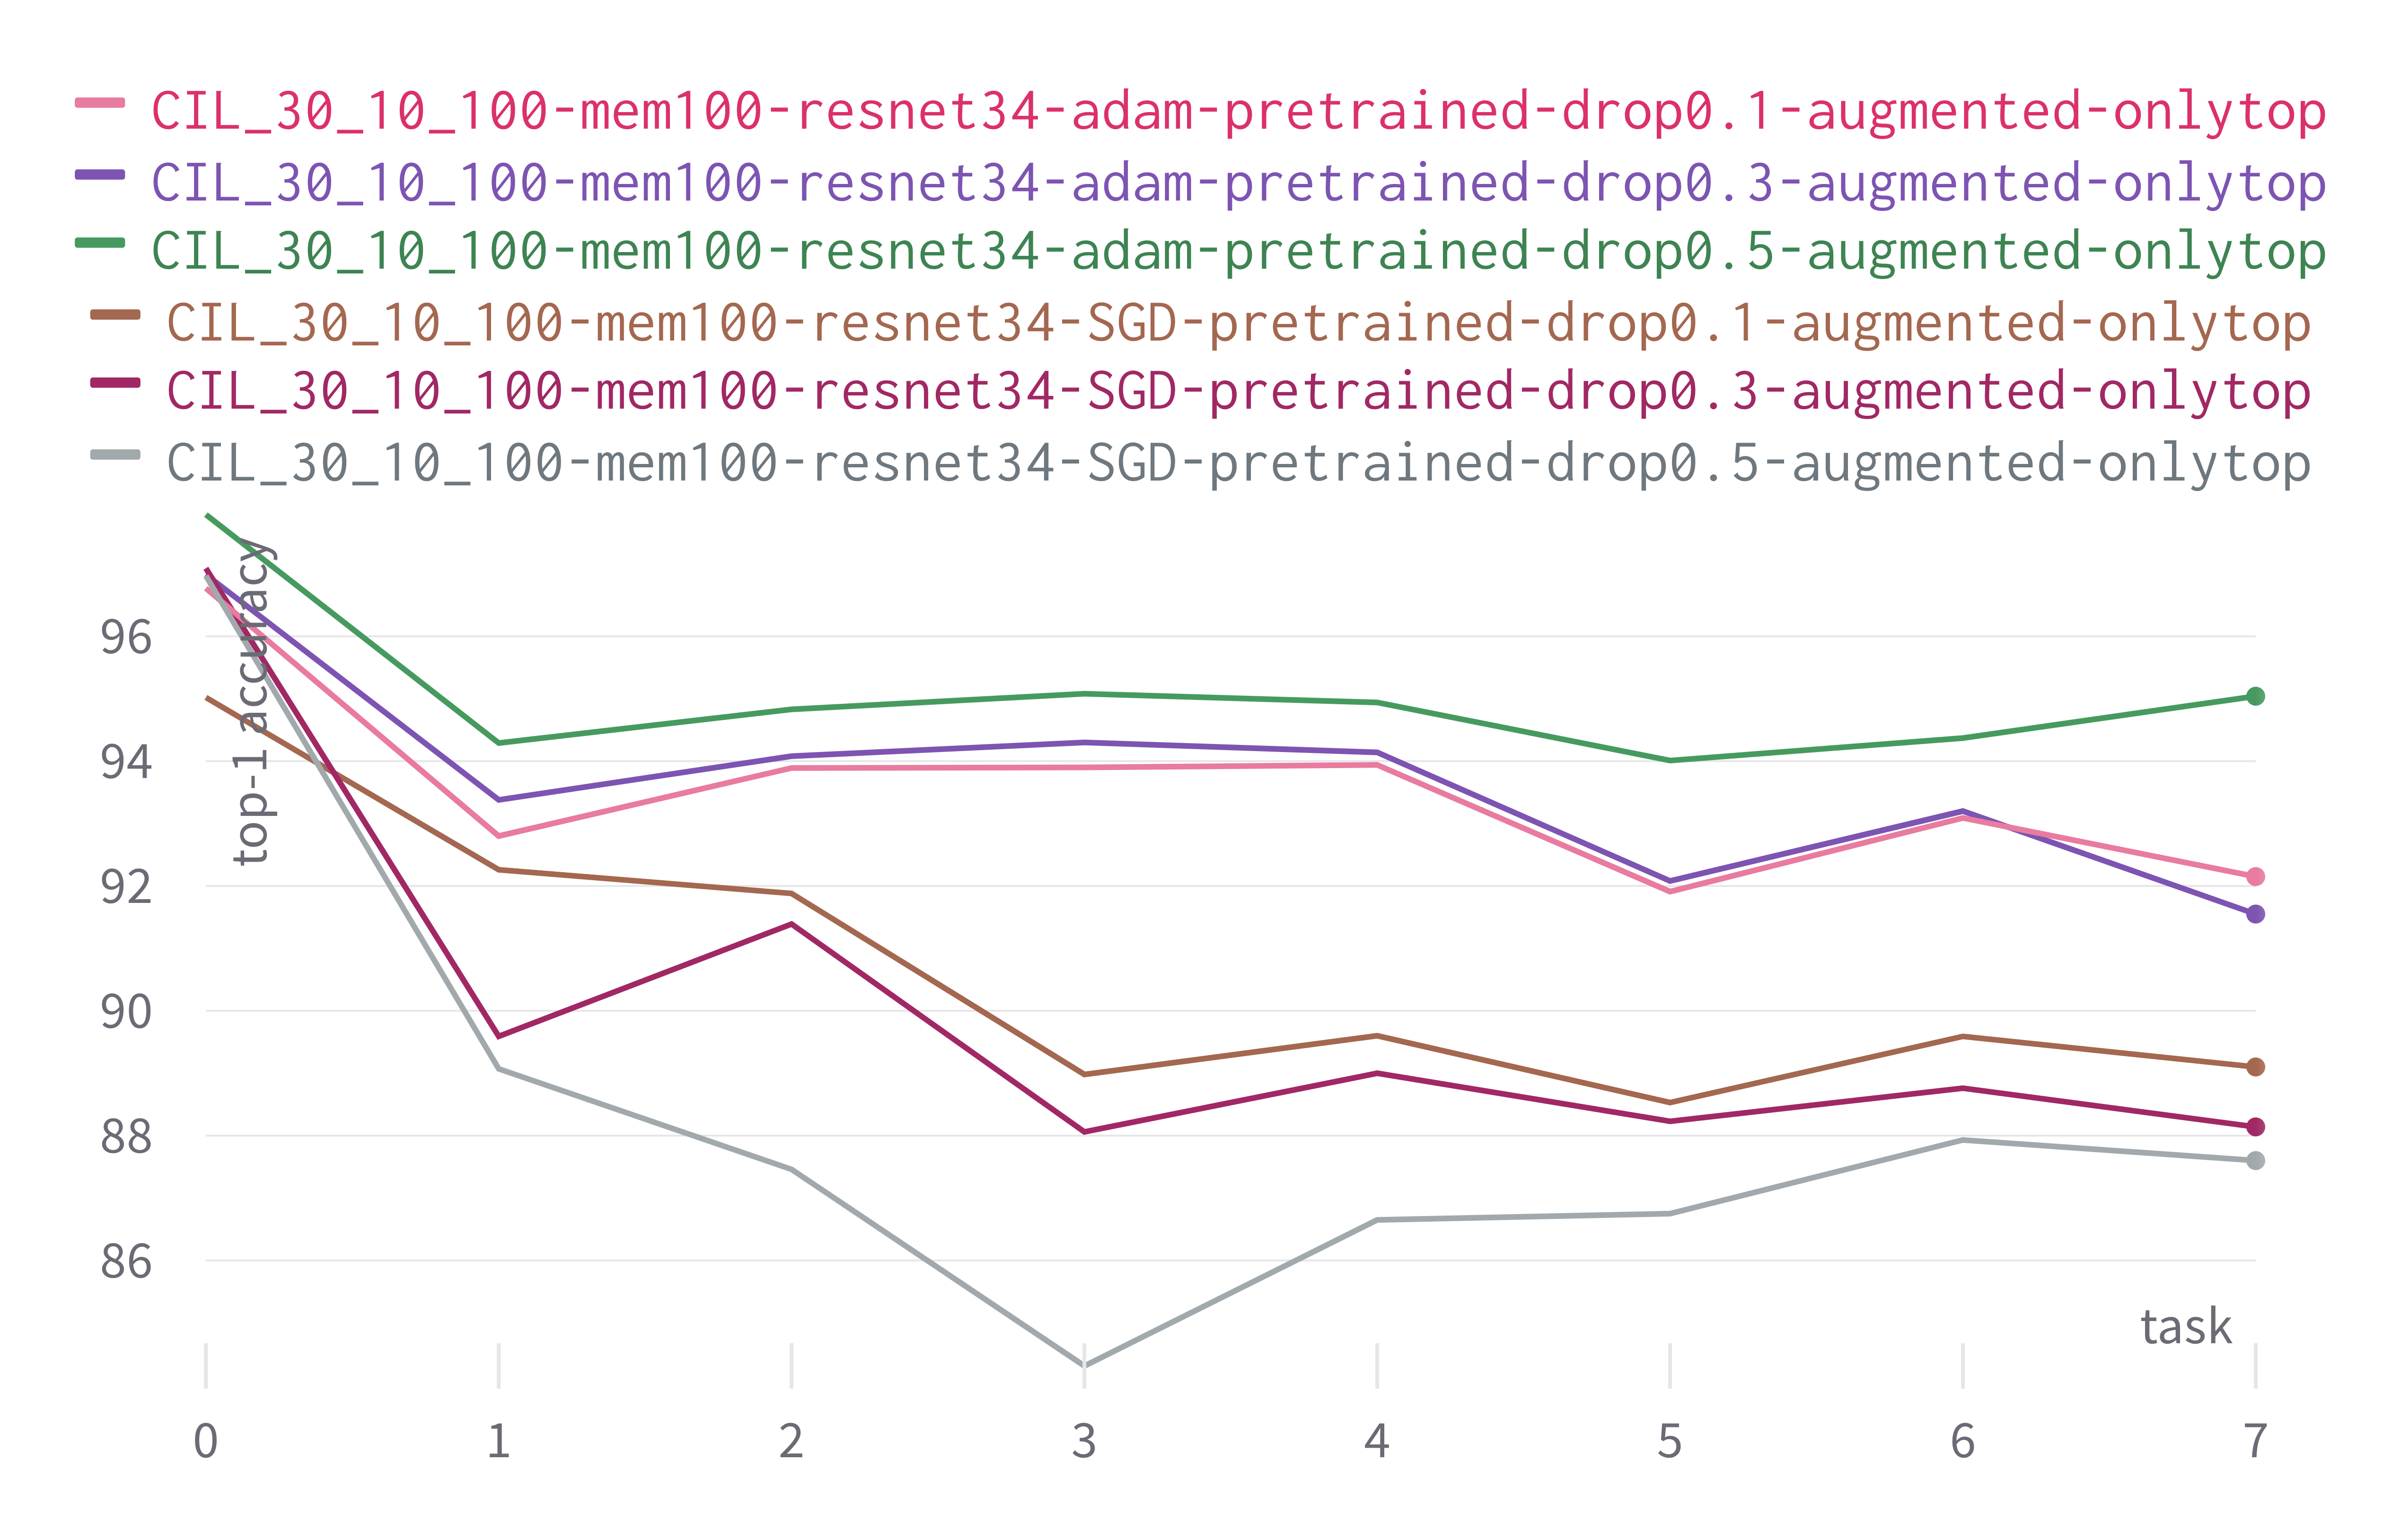
\includegraphics[width=0.50\textwidth]{images/exp/exp4-top1.png} }}%
    %\qquad
	\subfloat[\centering Top-5 accuracy]{{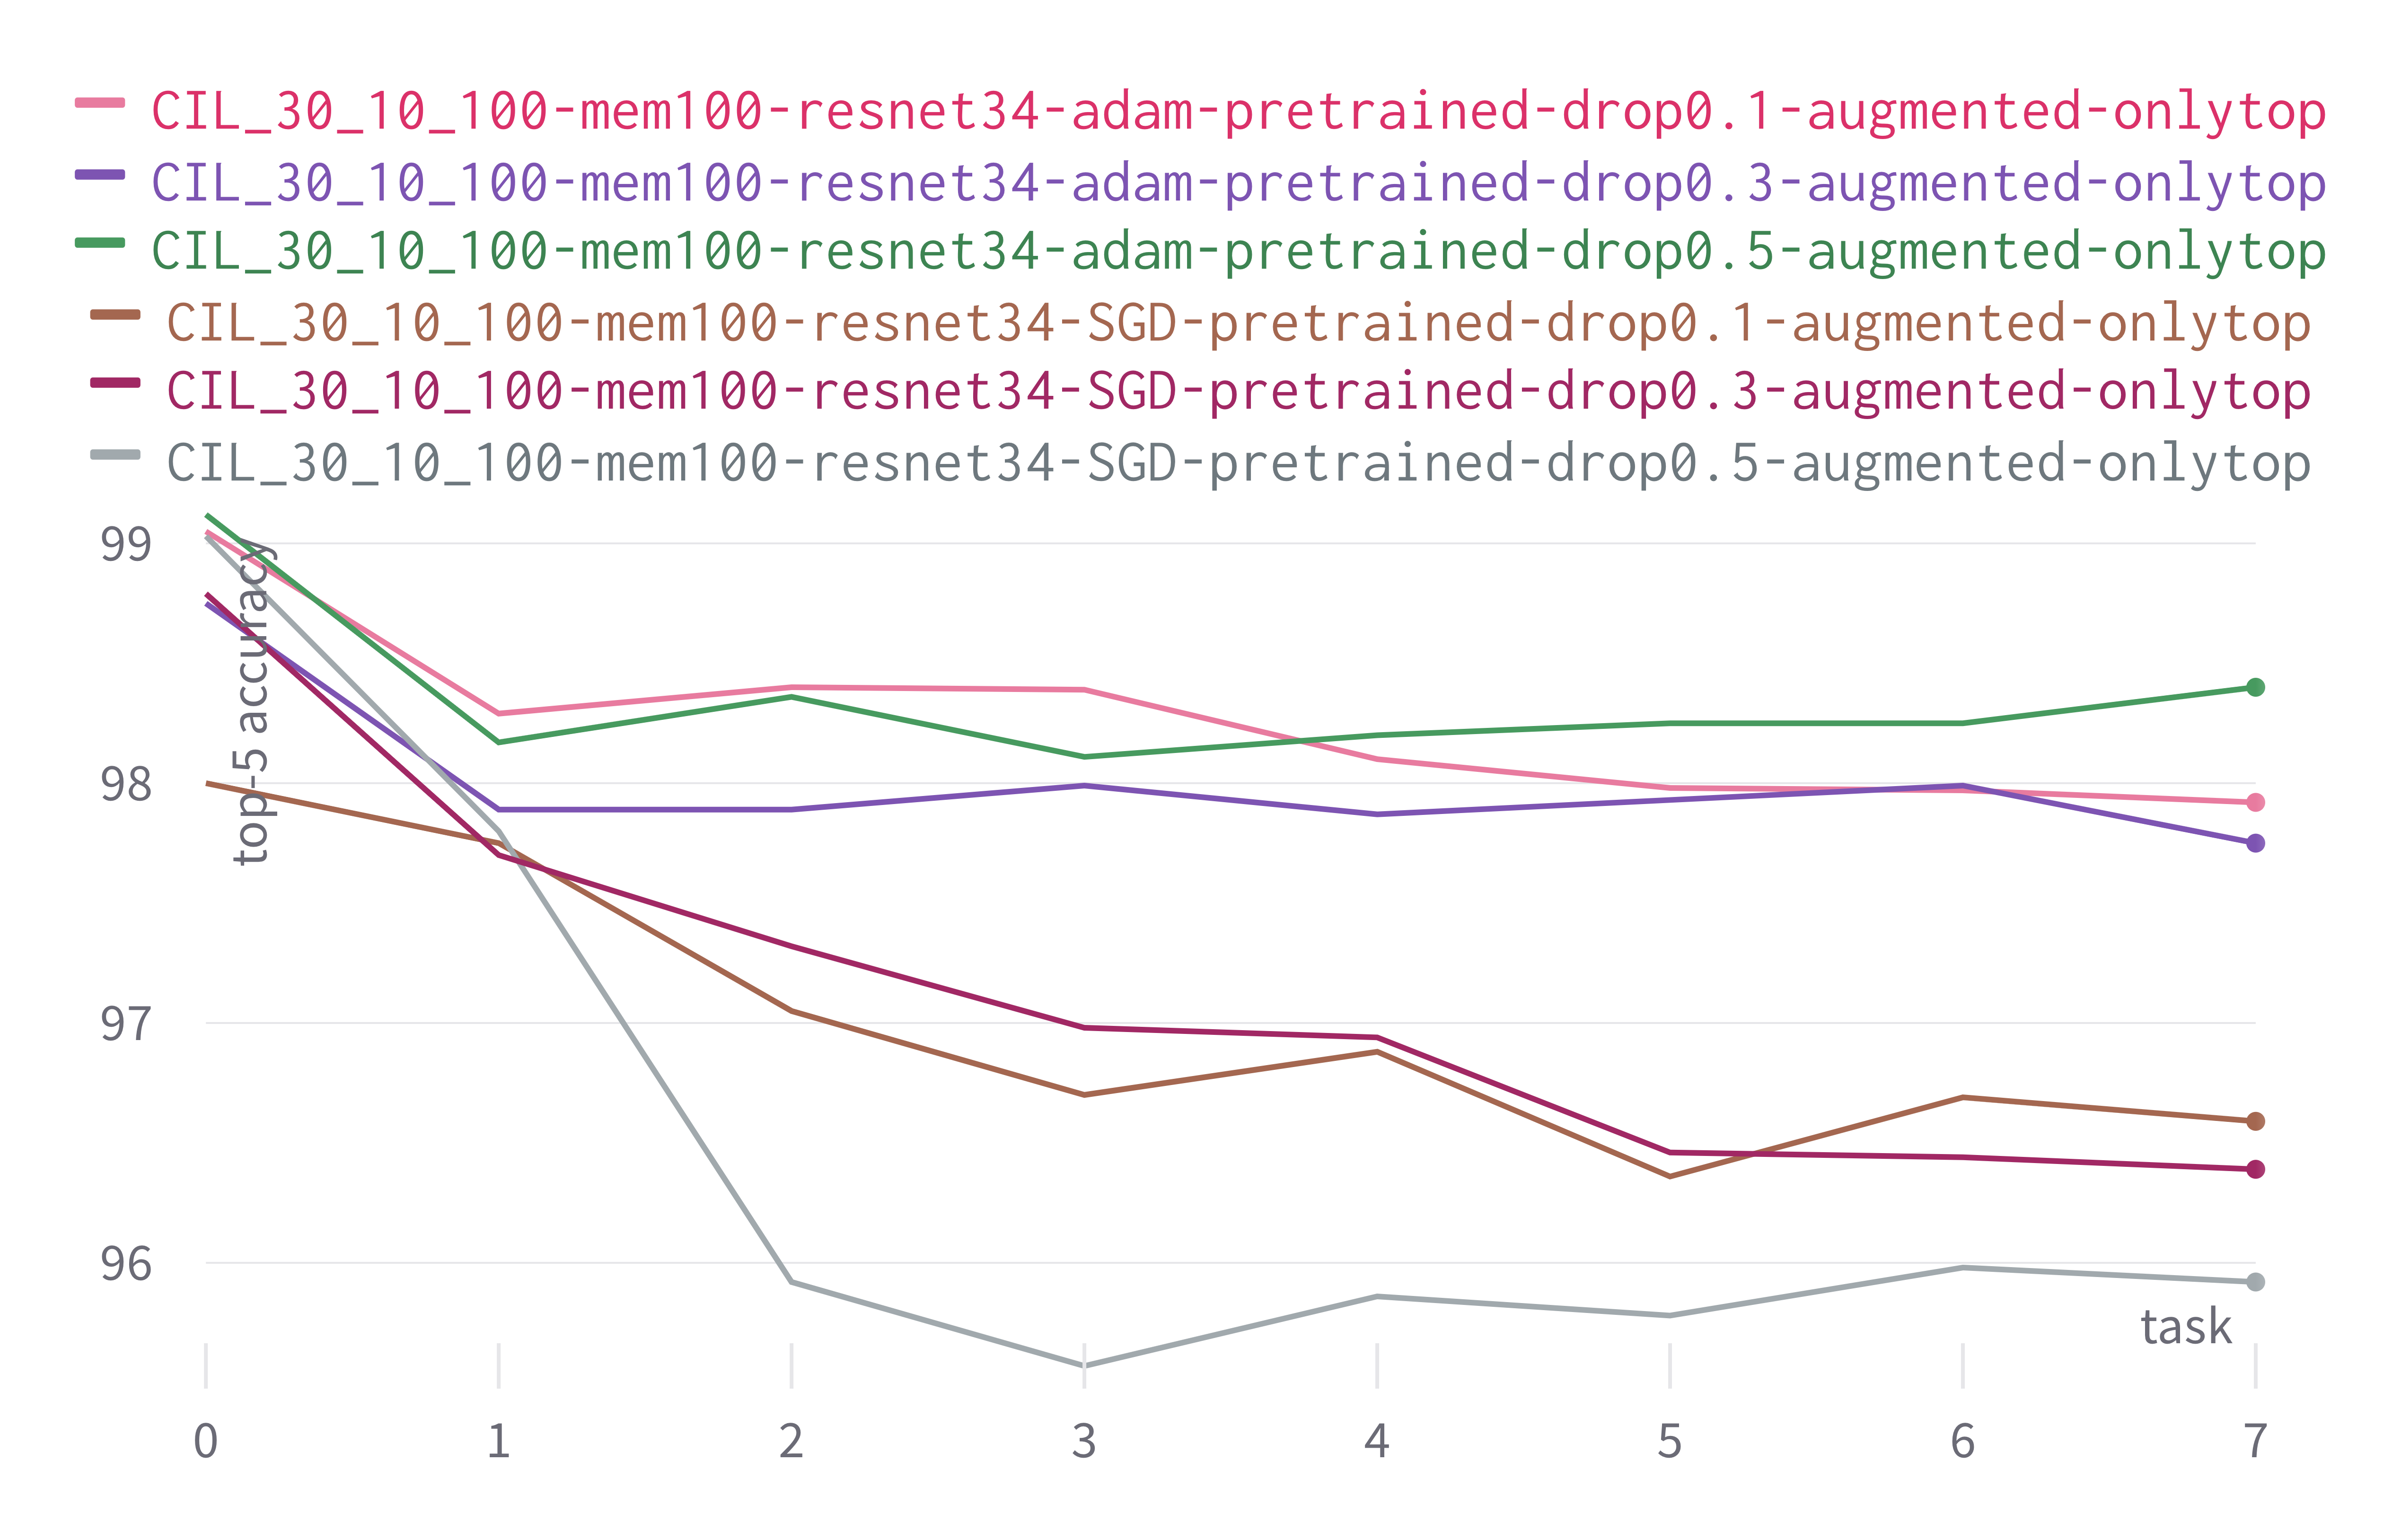
\includegraphics[width=0.50\textwidth]{images/exp/exp4-top5.png} }}%
	\caption{Comparison of models trained using SGD and Adam optimizers. Top-1 and top-5 accuracy at each task}%
	\label{fig:exp4}%
\end{figure}

\begin{table}[H]
    \centering
    \centerline{
    \begin{tabular}{c|c|c|c|c}
        \hline
        \textbf{Model} &
        \textbf{Dropout} &
        \textbf{Optimizer} &
        \textbf{Top-1} & 
        \textbf{Top-5} \\
        \textbf{name} &
        \textbf{rate} &
        \textbf{method} &
        \textbf{acc. (\%)} & 
        \textbf{acc. (\%)} \\
        \hline
        \hline
SGD-drop0.1-augmented-onlytop&0.1&SGD&89.1&96.59\\
SGD-drop0.3-augmented-onlytop&0.3&SGD&88.14&96.39\\
SGD-drop0.5-augmented-onlytop&0.5&SGD&87.6&95.92\\
\hline
adam-drop0.1-augmented-onlytop&0.1&Adam&92.15&97.92\\
adam-drop0.3-augmented-onlytop&0.3&Adam&91.55&97.75\\
adam-drop0.5-augmented-onlytop&0.5&Adam&\textbf{95.04}&\textbf{98.4}\\
        \hline
    \end{tabular}}
    \caption{Comparison of models trained using SGD and Adam optimizers. Top-1 and Top-5 accuracy at task 7.}
    \label{table:exp4}
\end{table}

\begin{figure}[H]
	\centering
	\subfloat[\centering Accuracy on the training set]{{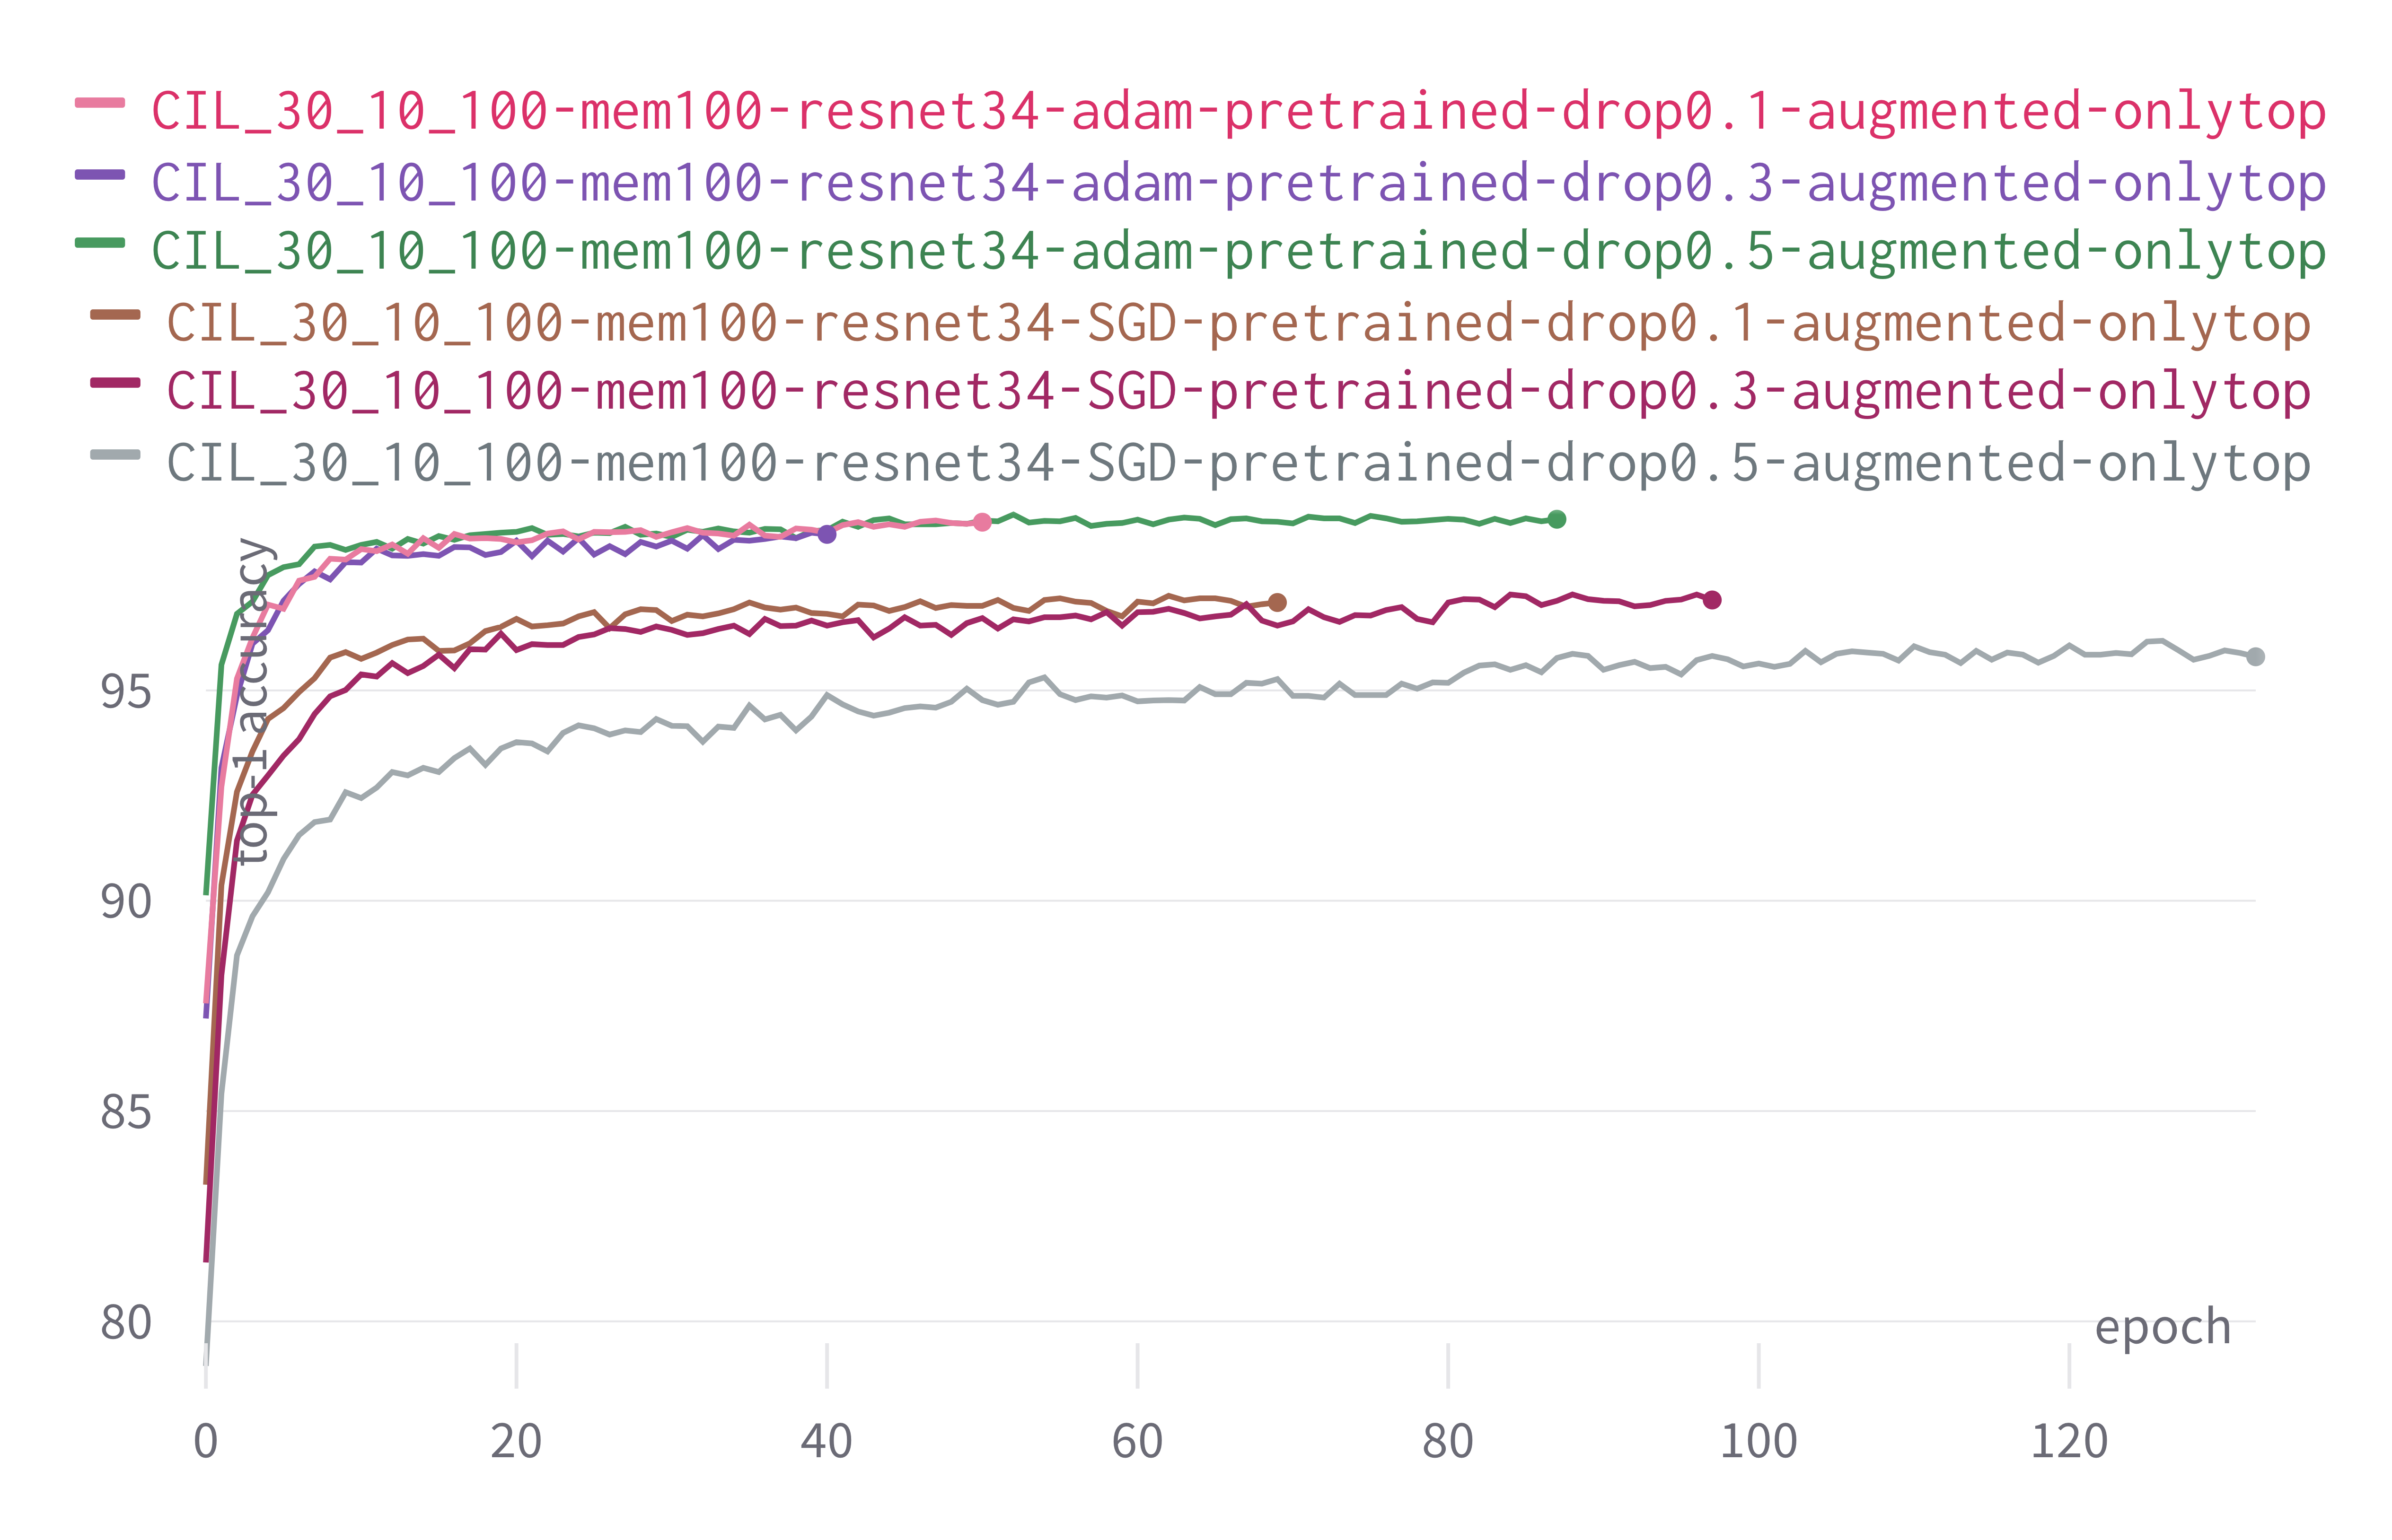
\includegraphics[width=0.50\textwidth]{images/exp/exp4-train.png} }}%
    %\qquad
	\subfloat[\centering Accuracy on the validation set]{{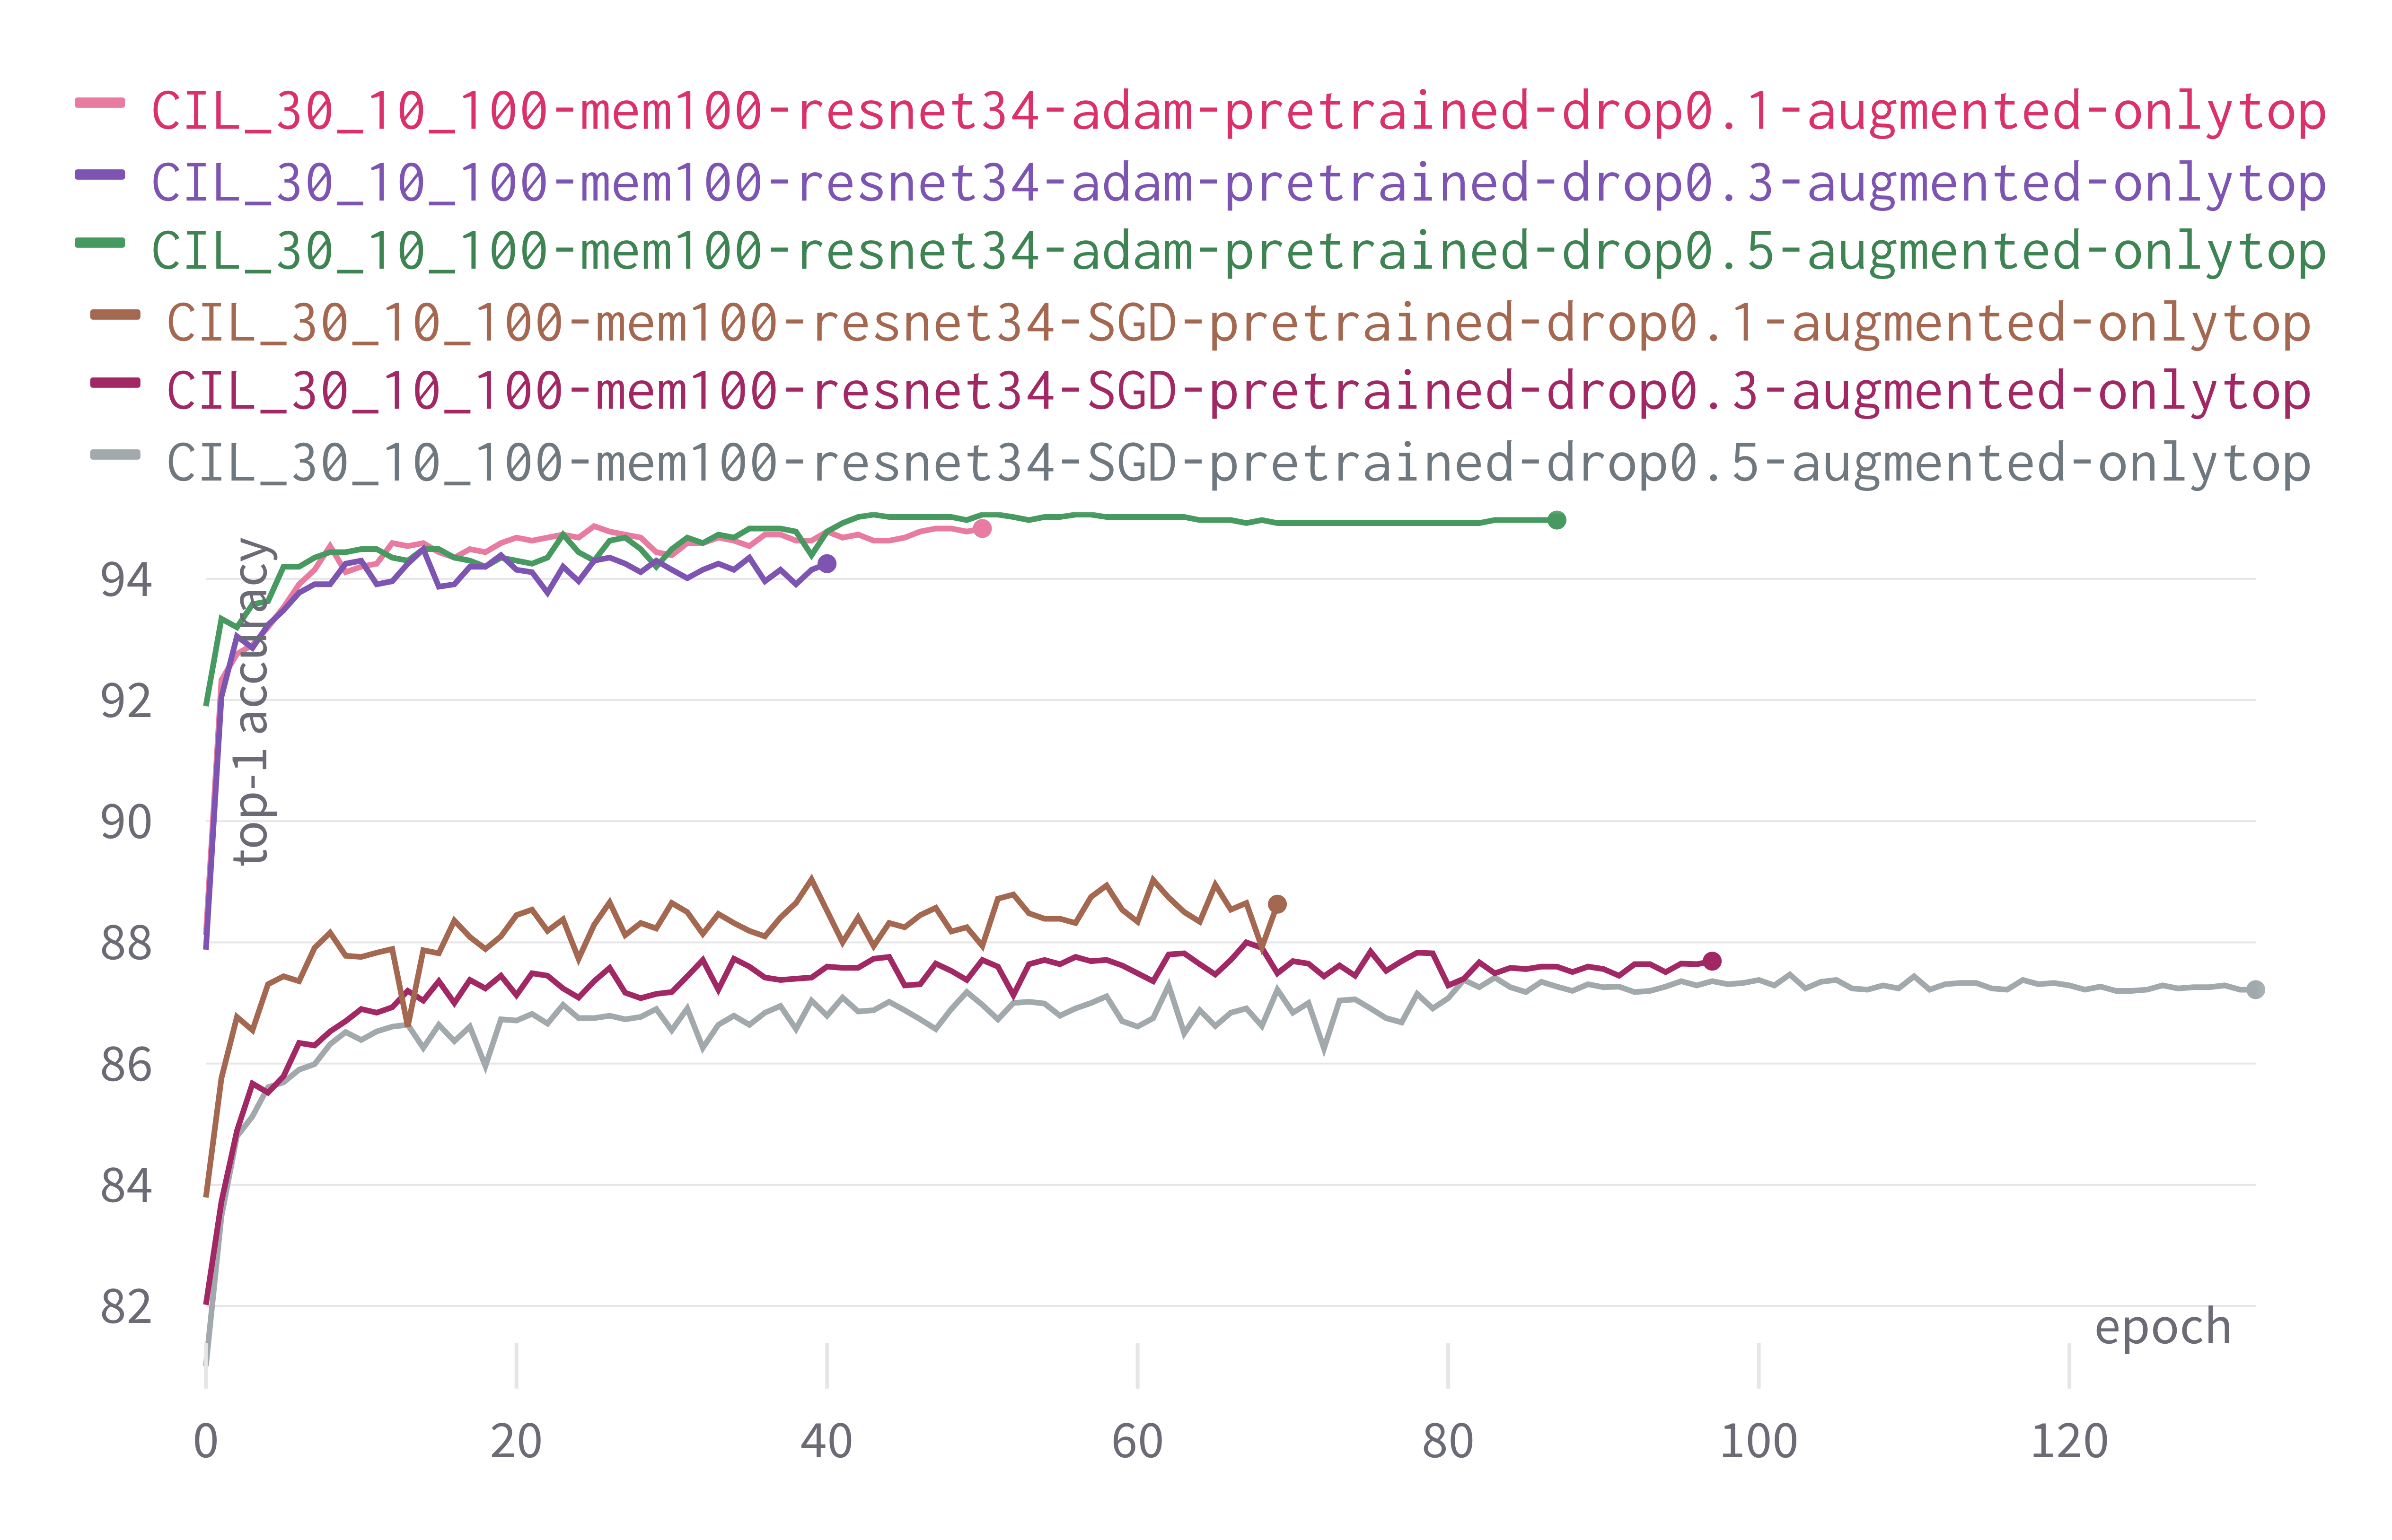
\includegraphics[width=0.50\textwidth]{images/exp/exp4-val.png} }}%
	\caption{Comparison of models trained using SGD and Adam optimizers. The images show the training history of models at task 7, comparing the top-1 accuracy at each training epoch evaluated on the training and validation set.}%
	\label{fig:exp4-train_val}%
\end{figure}

%\newpage

\subsubsection{Type 2 baseline}
\label{sec:exp-baseline2}
To address the problems relative to the type 1 baseline, the models tested in the previous section are compared with the type 2 baseline described in \autoref{sec:method-baseline2}.
This new baseline is trained on the same dataset used for CIL models and consists in fine-tuning ResNet-152 pretrained on ImageNet to the task of logo classification.
This new baseline uses data augmentation, a dropout layer before the FC layer and the Adam optimizer.

Considering the top-1 and top-5 accuracy on the test set, the performance of CIL models and type 2 baselines are compared in \autoref{table:baseline2}.
As we can see, the performance of the best CIL model is very similar to that of the baseline, but the latter still performs worse, even if only slightly.
Although this new baseline alleviates the problem of the number of model parameters, this issue is still present, as shown in \autoref{table:baseline2-params}.

\begin{table}[H]
    \centering
    \centerline{
    \begin{tabular}{c|c|c}
        \hline
        \textbf{Model} &
        \textbf{Dropout} &
        \textbf{Top-1} \\
        \textbf{name} &
        \textbf{rate} &
        \textbf{acc. (\%)} \\
        \hline
\hline
adam-drop0.1-augmented-onlytop&0.1&92.15\\
adam-drop0.3-augmented-onlytop&0.3&91.55\\
adam-drop0.5-augmented-onlytop&0.5&\textbf{95.04}\\
\hline
BASELINE\_2-drop0.1-augmented-onlytop&0.1&82.35\\
BASELINE\_2-drop0.3-augmented-onlytop&0.3&94.11\\
BASELINE\_2-drop0.5-augmented-onlytop&0.5&88.23\\
\hline 
    \end{tabular}}
    \caption{Performance comparison between CIL models and type 2 baselines. Top-1 accuracy calculated on the test set composed of 100 classes.}
    \label{table:baseline2}
\end{table}

\begin{table}[H]
    \centering
    \centerline{
    \begin{tabular}{c|c}
        \hline
        \textbf{Model} &
        \textbf{\#Params} \\
        \textbf{name} &
        \textbf{(M)} \\
        \hline
adam-drop0.1-augmented-onlytop&170\\
adam-drop0.3-augmented-onlytop&170\\
adam-drop0.5-augmented-onlytop&170\\
\hline
BASELINE\_2-drop0.1-augmented-onlytop&60\\
BASELINE\_2-drop0.3-augmented-onlytop&60\\
BASELINE\_2-drop0.5-augmented-onlytop&60\\
\hline 
    \end{tabular}}
    \caption{Comparison between CIL models and type 2 baselines considering the number of model parameters.}
    \label{table:baseline2-params}
\end{table}

%\newpage
\subsubsection{Type 3 baseline}
The type 3 baseline aims to solve the problem of the number of model parameters.
In fact, this approach (described in \autoref{sec:method-baseline3}) defines the baseline architecture using the DER algorithm in the same setup as the CIL classifier, thus having an identical architecture for both the CIL model and the baseline.
This ensures that the number of model parameters is the same.
The baseline is then trained using data augmentation, regularization, the Adam optimizer and the same dataset.

The performance of the CIL models and this new baseline are compared considering the top-1 accuracy on the test set.
As we can see from \autoref{table:baseline3}, the type 3 baseline achieves better performance than the CIL model.

This makes it possible to compare the drop in performance using an incremental learning setup against a standard setup.
As shown in \autoref{table:baseline3}, this gap is present, with a 3\% drop in top-1 accuracy, but it is expected using an incremental learning setup.
However, a 3\% drop is acceptable when considering the advantages of an incremental learning approach.

\begin{table}[H]
    \centering
    \centerline{
    \begin{tabular}{c|c|c}
        \hline
        \textbf{Model} &
        \textbf{Dropout} &
        \textbf{Top-1} \\
        \textbf{name} &
        \textbf{rate} &
        \textbf{acc. (\%)} \\
        \hline
\hline
adam-drop0.1-augmented-onlytop&0.1&92.15\\
adam-drop0.3-augmented-onlytop&0.3&91.55\\
adam-drop0.5-augmented-onlytop&0.5&95.04\\
\hline\
BASELINE\_3-drop0.1-augmented-onlytop&0.1&\textbf{98.52}\\
BASELINE\_3-drop0.3-augmented-onlytop&0.3&97.05\\
BASELINE\_3-drop0.5-augmented-onlytop&0.5&97.64\\
\hline 
    \end{tabular}}
    \caption{Top-1 accuracy of CIL models and type 3 baselines considering all the 100 classes of the test set.}
    \label{table:baseline3}
\end{table}

%\newpage
\subsubsection{Pruning (100 classes)}
An important aspect discussed in \autoref{sec:method-pruning} is the number of model parameters.
All models tested up to this point add approximately 22 million parameters with each new iteration of incremental learning, thus reaching 170 million parameters at task 7 (22 million for the initial task and 7 iterations of incremental learning).

The following experiments are designed to assess the pruning capacity of the channel-level masks and the drop in performance obtained with this method.
To this end, the pruned models are compared with those described in the previous section.
An important difference in the training procedure of the pruned model consists in monitoring the loss on the validation set instead of the accuracy.
This is done because the validation loss decreases with increasing sparsity of the model, and we want to encourage a more sparse model given the same accuracy on the validation set.

The results of the performance comparison are shown in \autoref{fig:exp5} and \autoref{table:exp5}. As we can see, the drop in performance is negligible, with some pruned models performing even better than un-pruned ones.
This can be explained by considering pruning as a regularization technique, in fact decreasing the number of parameters effectively reduces the Vapnik-Chervonenkis (VC) dimension \cite{vapnik1999nature}.
%It is important to emphasize that these models are trained considering the top-100 classes, so it is essential to test the scalability of models to the entire dataset.

The results of pruning are shown in \autoref{fig:exp5-params} and \autoref{table:exp5-params}.
As we can see, this technique is very effective.
The final number of model parameters is reduced by almost a factor of 5x.
Note that the models not using pruning already exceed the total number of parameters of those using pruning from task 1 (43 for the un-pruned vs. 32 for pruned approx.).

Other interesting insights emerge by analyzing the training history of the models at task 0.
The loss function of the DER algorithm (see \autoref{eq:final_der_loss}) is defined as the sum of: the loss of the classifier, the loss of the auxiliary classifier and loss related to the pruning masks.
In \autoref{fig:exp5-loss} we can see the classification loss (c), sparsity loss (d) and final loss (b) of the model for each training epoch at task 0.
Initially, the classification loss (c) tends to decrease, but as the training epochs advance, the sparsity loss (d) increasingly masks the channels of the convolutional layers.
This leads to a continuous decrease in parameters, but the classification (c) is significantly affected.
The deterioration of performance can also be seen in the top-1 accuracy (a) on the validation set.

\begin{figure}[H]
	\centering
	\subfloat[\centering Top-1 accuracy]{{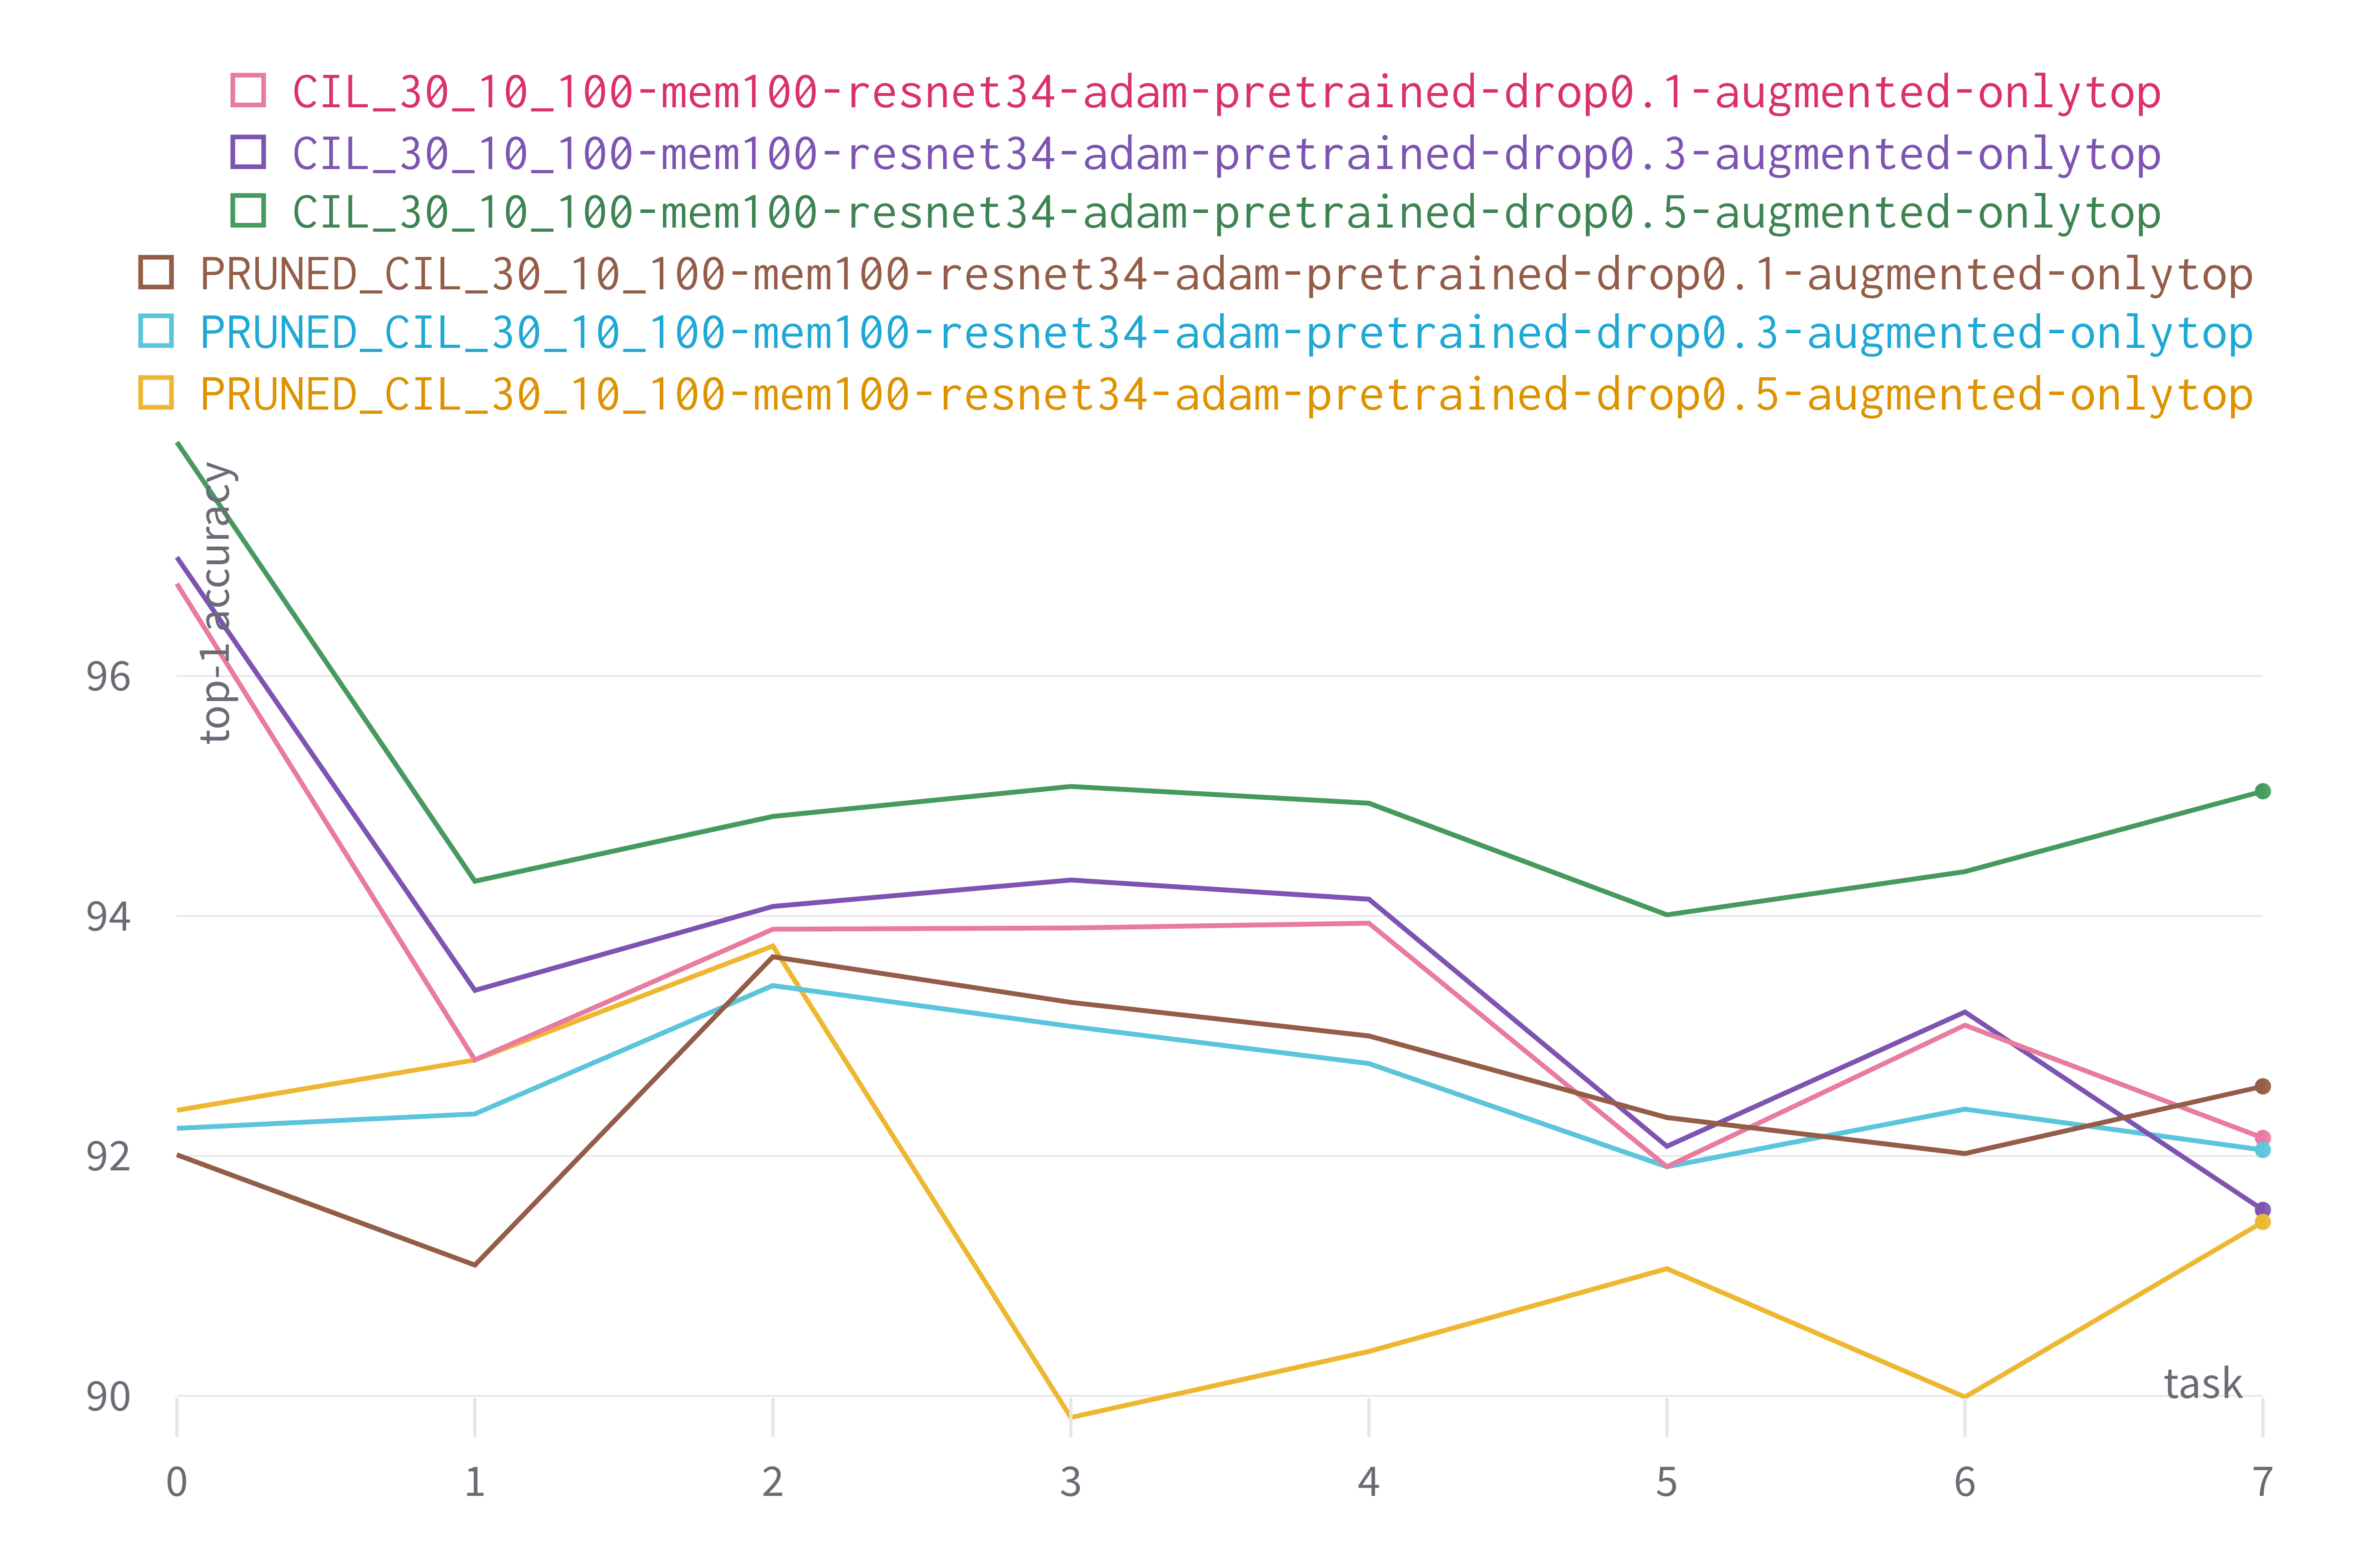
\includegraphics[width=0.50\textwidth]{images/exp/exp5-top1.png} }}%
    %\qquad
	\subfloat[\centering Top-5 accuracy]{{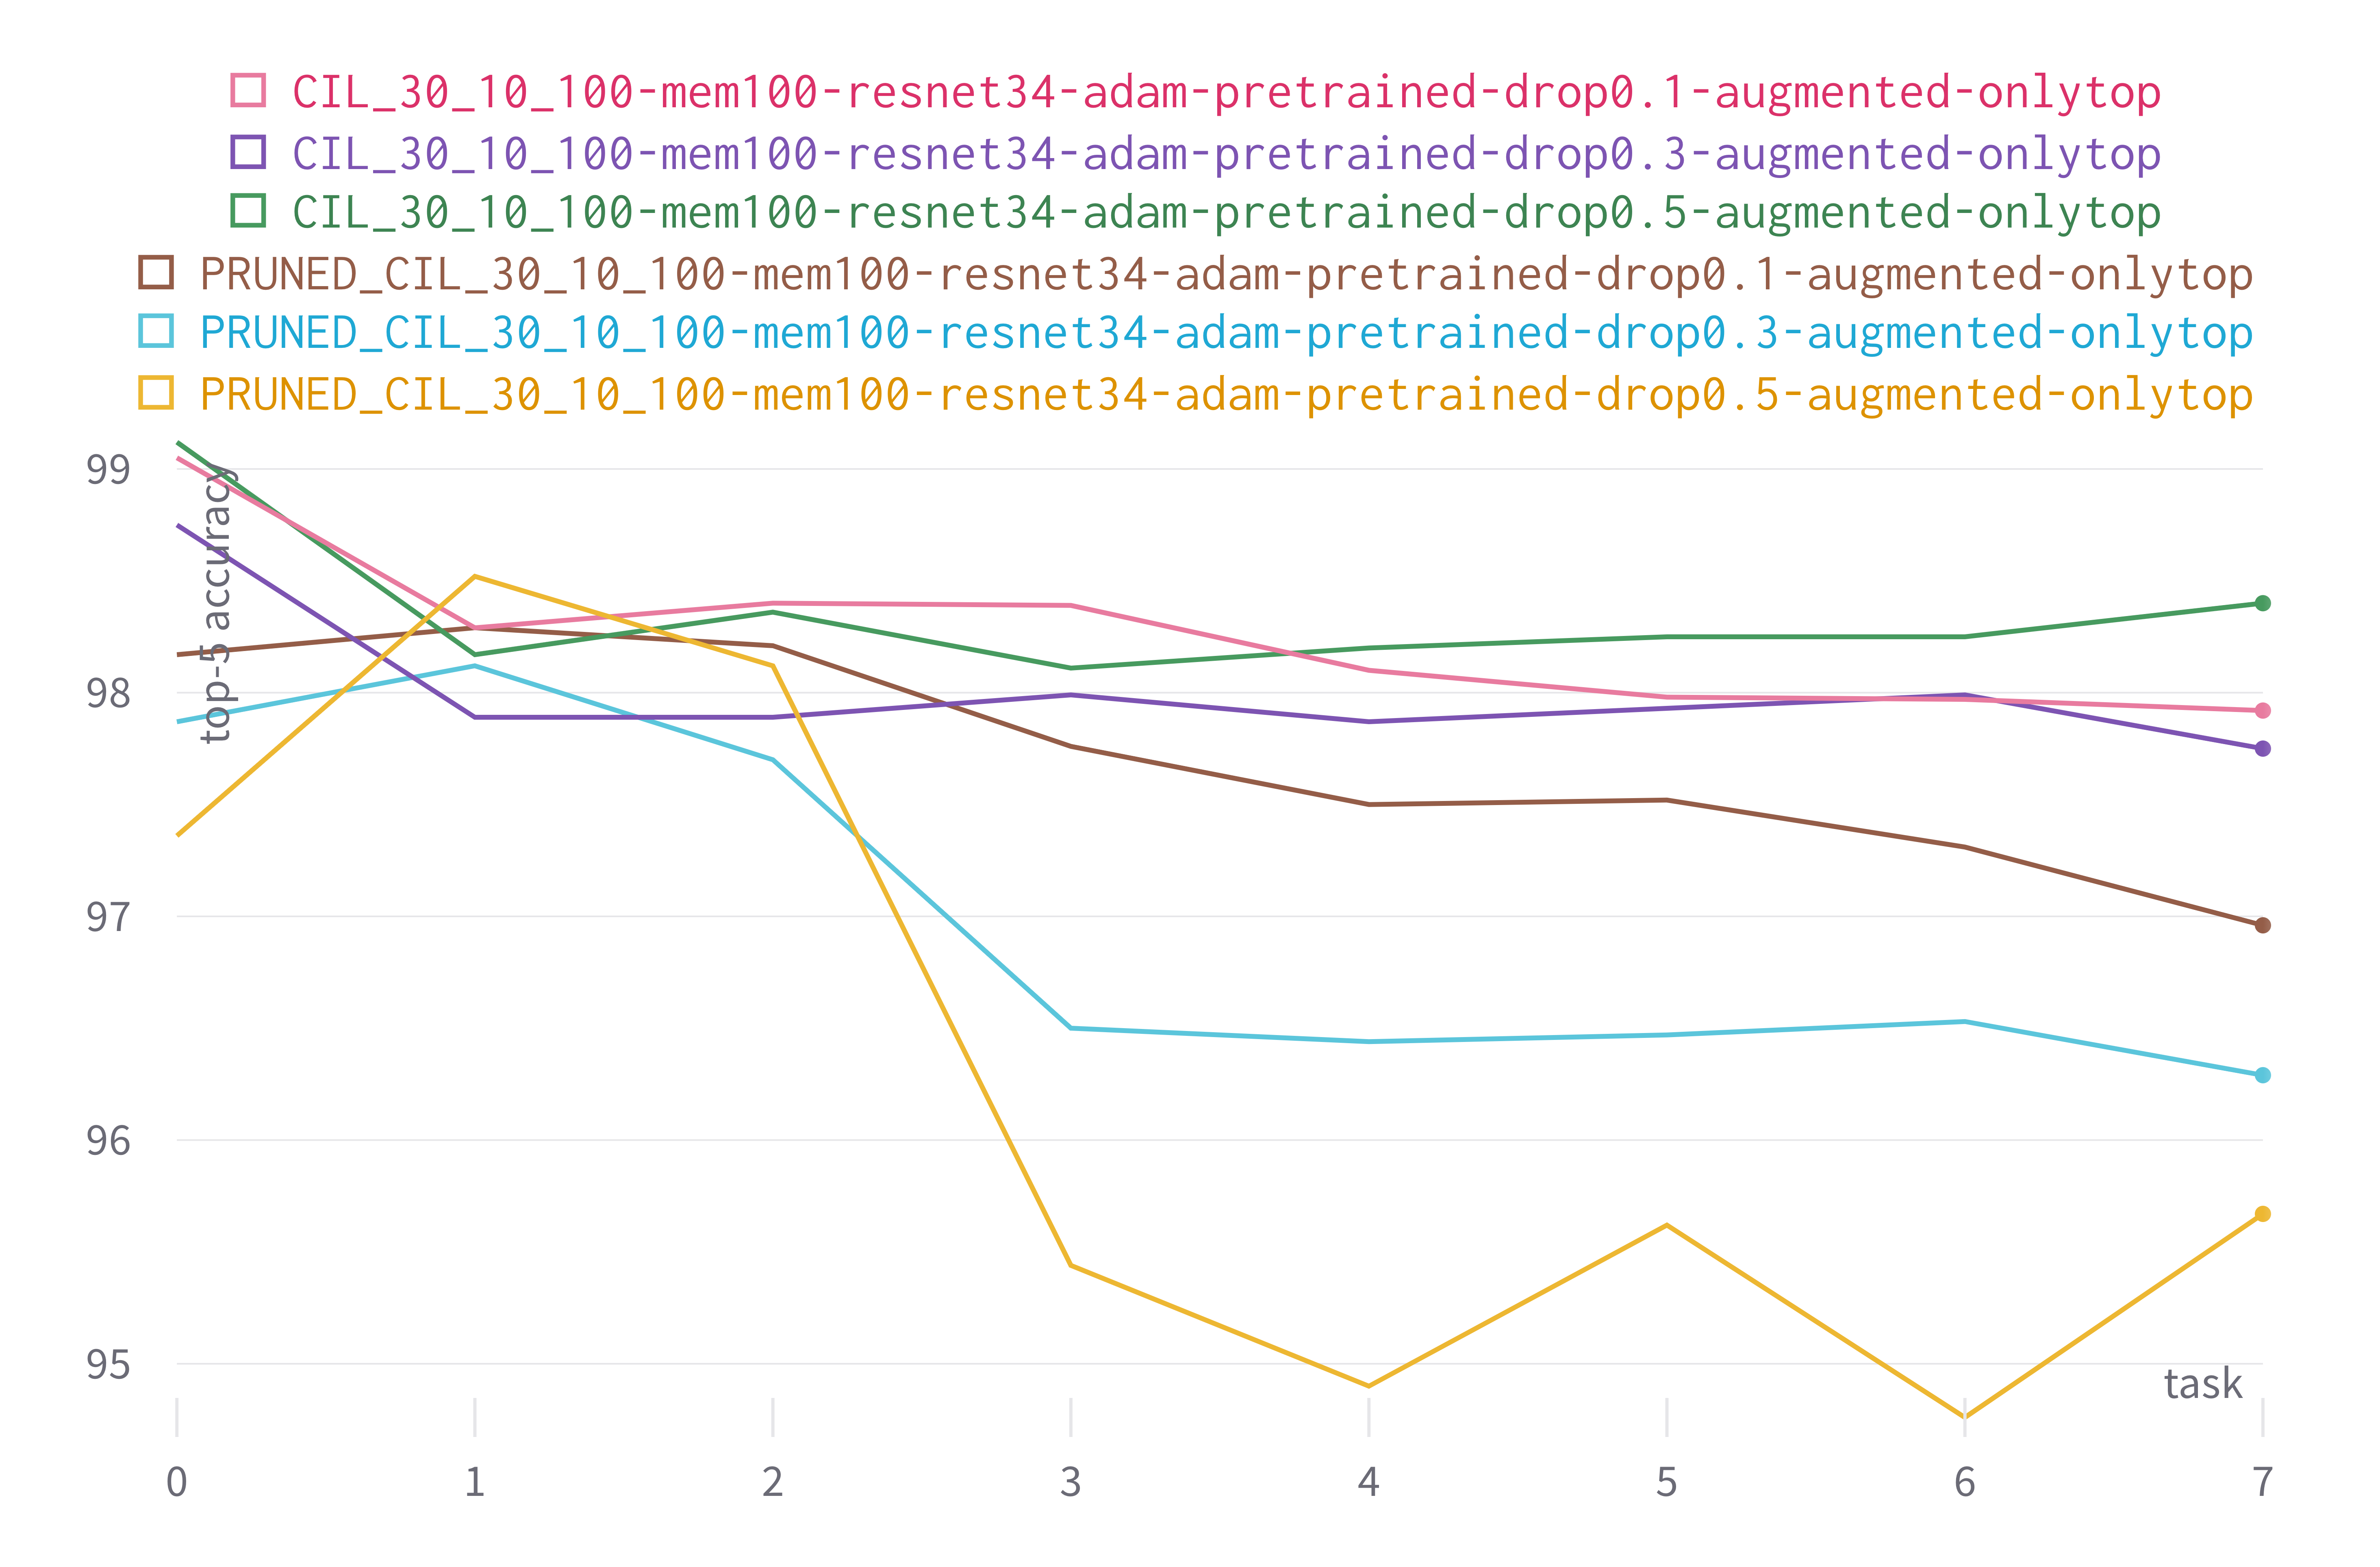
\includegraphics[width=0.50\textwidth]{images/exp/exp5-top5.png} }}%
	\caption{Performance comparison between pruned models and un-pruned ones considering top-1 and top-5 at each task.}%
	\label{fig:exp5}%
\end{figure}


\begin{table}[H]
    \centering
    \centerline{
    \begin{tabular}{c|c|c|c|c}
        \hline
        \textbf{Model} &
        \textbf{Dropout} &
        \textbf{Pruning} &
        \textbf{Top-1} & 
        \textbf{Top-5} \\
        \textbf{name} &
        \textbf{rate} &
        &
        \textbf{acc. (\%)} & 
        \textbf{acc. (\%)} \\
        \hline
        \hline
drop0.1-augmented-onlytop&0.1&no&92.15&97.92\\
drop0.3-augmented-onlytop&0.3&no&91.55&97.75\\
drop0.5-augmented-onlytop&0.5&no&\textbf{95.04}&\textbf{98.4}\\
\hline
PRUNED-drop0.1-augmented-onlytop&0.1&yes&92.58&96.96\\
PRUNED-drop0.3-augmented-onlytop&0.3&yes&92.05&96.29\\
PRUNED-drop0.5-augmented-onlytop&0.5&yes&91.45&95.67\\
        \hline
    \end{tabular}}
    \caption{Performance comparison between the pruned models and the un-pruned ones. Top-1 and top-5 accuracy at task 7.}
    \label{table:exp5}
\end{table}

\begin{table}[ht]
\begin{minipage}{\textwidth}
    \begin{minipage}[b]{0.50\textwidth}
        \centering
        %\begin{figure}[H]
            \centering
            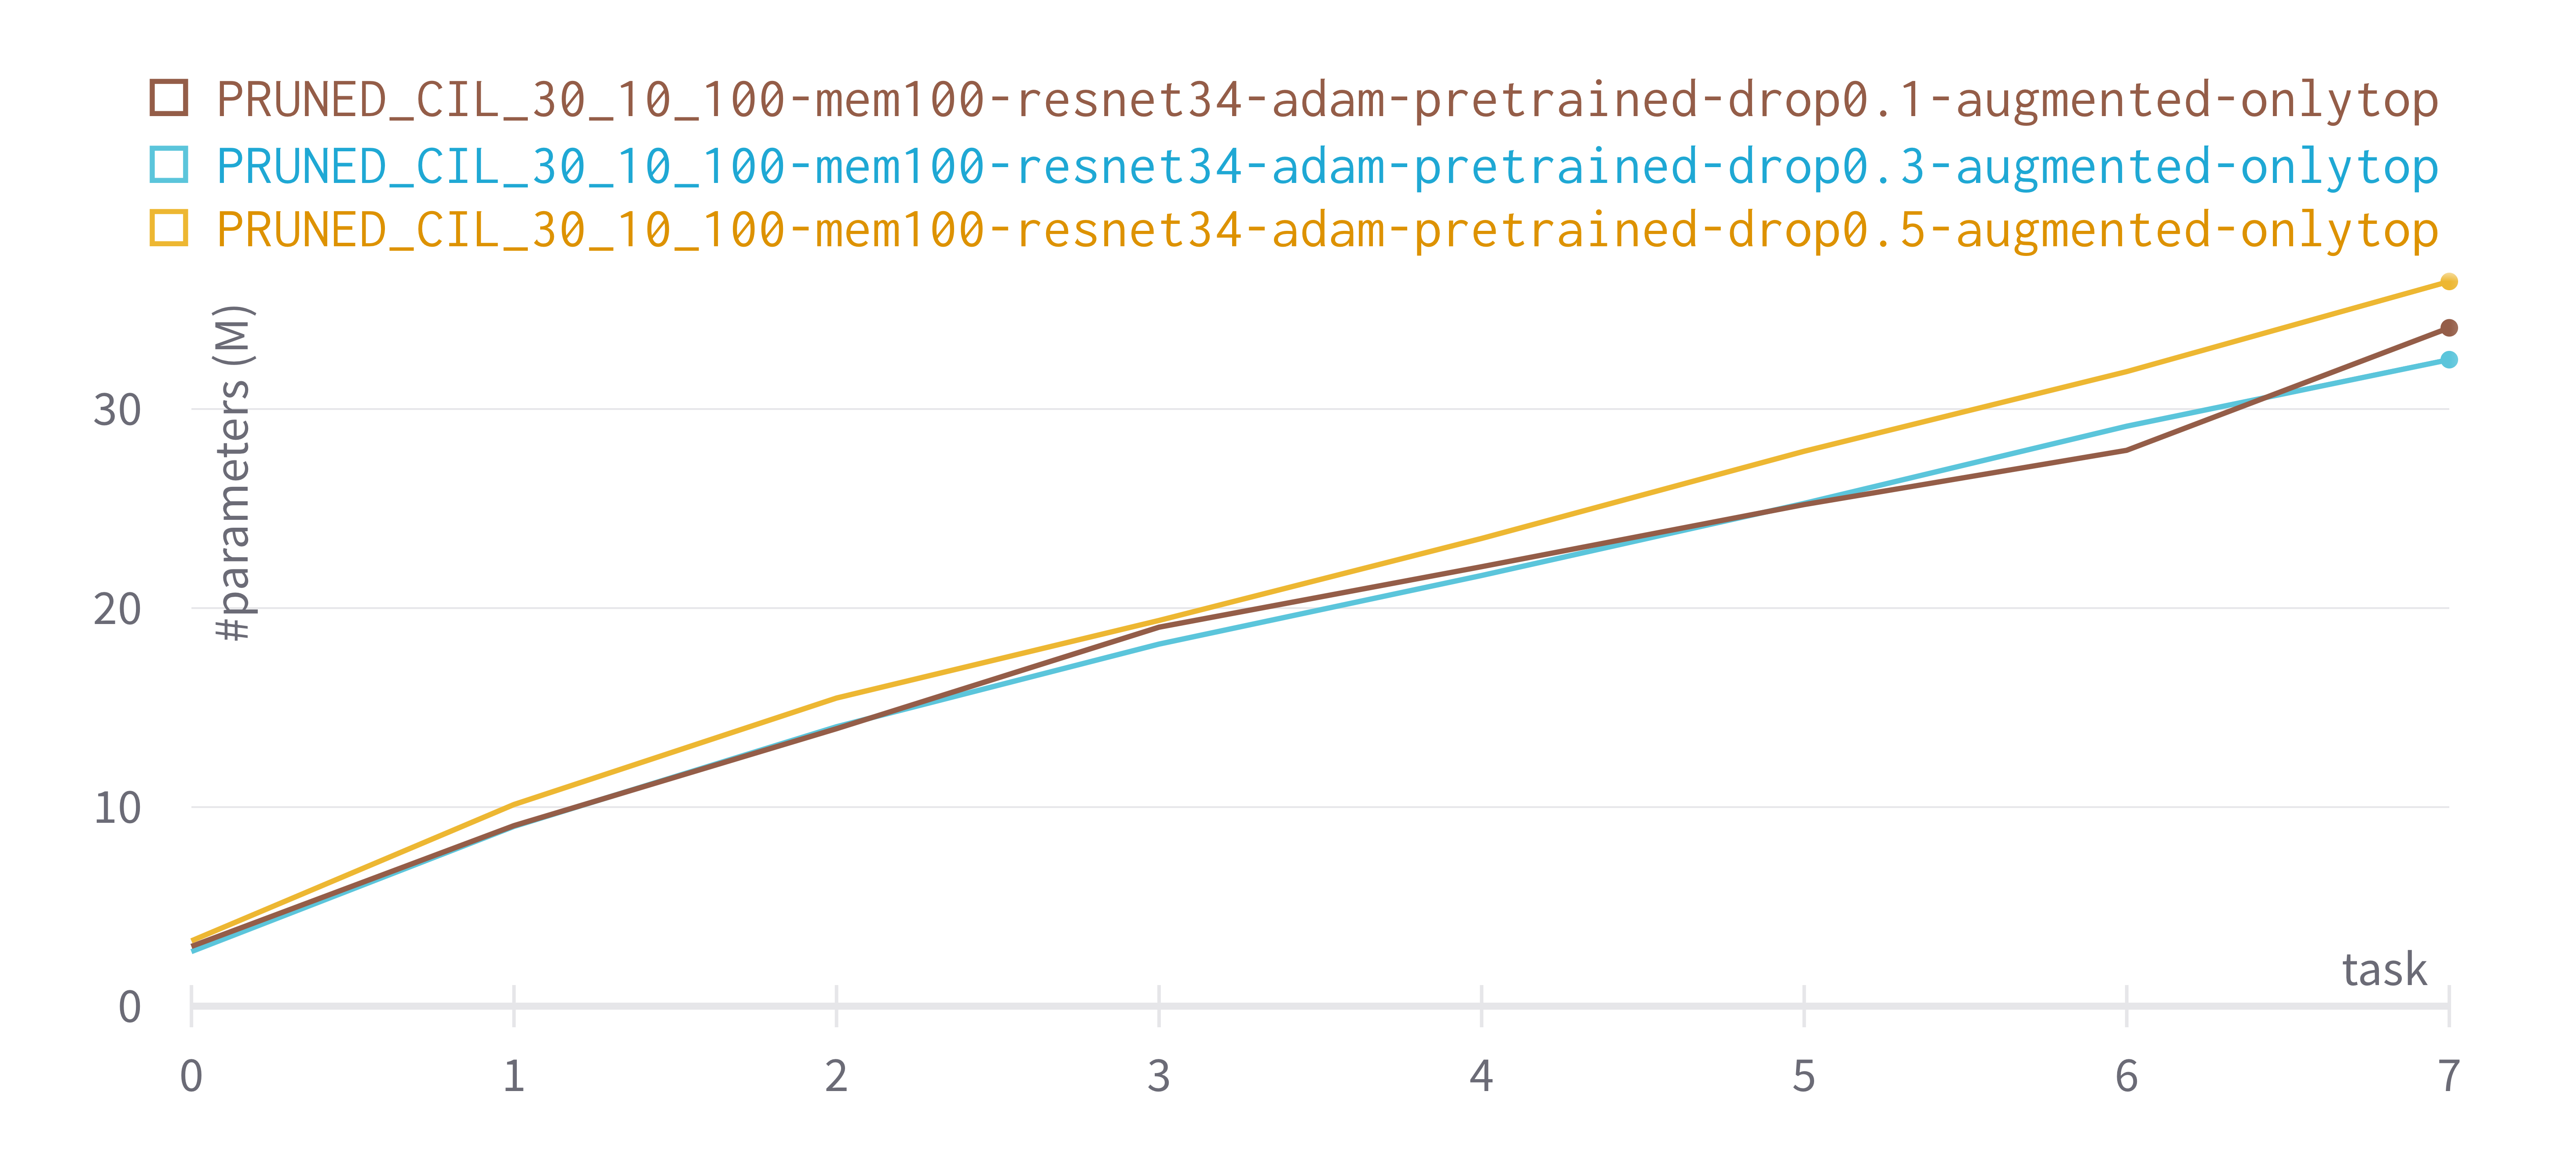
\includegraphics[width=1\textwidth]{images/exp/exp5-params.png}
            \captionof{figure}{Number of model parameters at each task using the pruning technique.}
            \label{fig:exp5-params}
        %\end{figure}
    \end{minipage}
    \hfill
    \begin{minipage}[b]{0.45\textwidth}                
        \begin{table}[H]
            \centering
            \centerline{
                \begin{tabular}{c|c}
                    \hline
                    \textbf{Model} &
                    \textbf{\#Params} \\
                    \textbf{name} &
                    \textbf{(M)} \\
                    \hline
                    \hline
        UNPRUNED-drop0.1&170\\
        UNPRUNED-drop0.3&170\\
        UNPRUNED-drop0.5&170\\
        \hline
        PRUNED-drop0.1&34.08\\
        PRUNED-drop0.3&32.48\\
        PRUNED-drop0.5&36.41\\
                    \hline
                \end{tabular}}
                \caption{Number of model parameters at task 7.}
                \label{table:exp5-params}
        \end{table}
    \end{minipage}
\end{minipage}
\end{table}
    
\begin{figure}[H]
	\centering
	\subfloat[\centering Top-1 accuracy]{{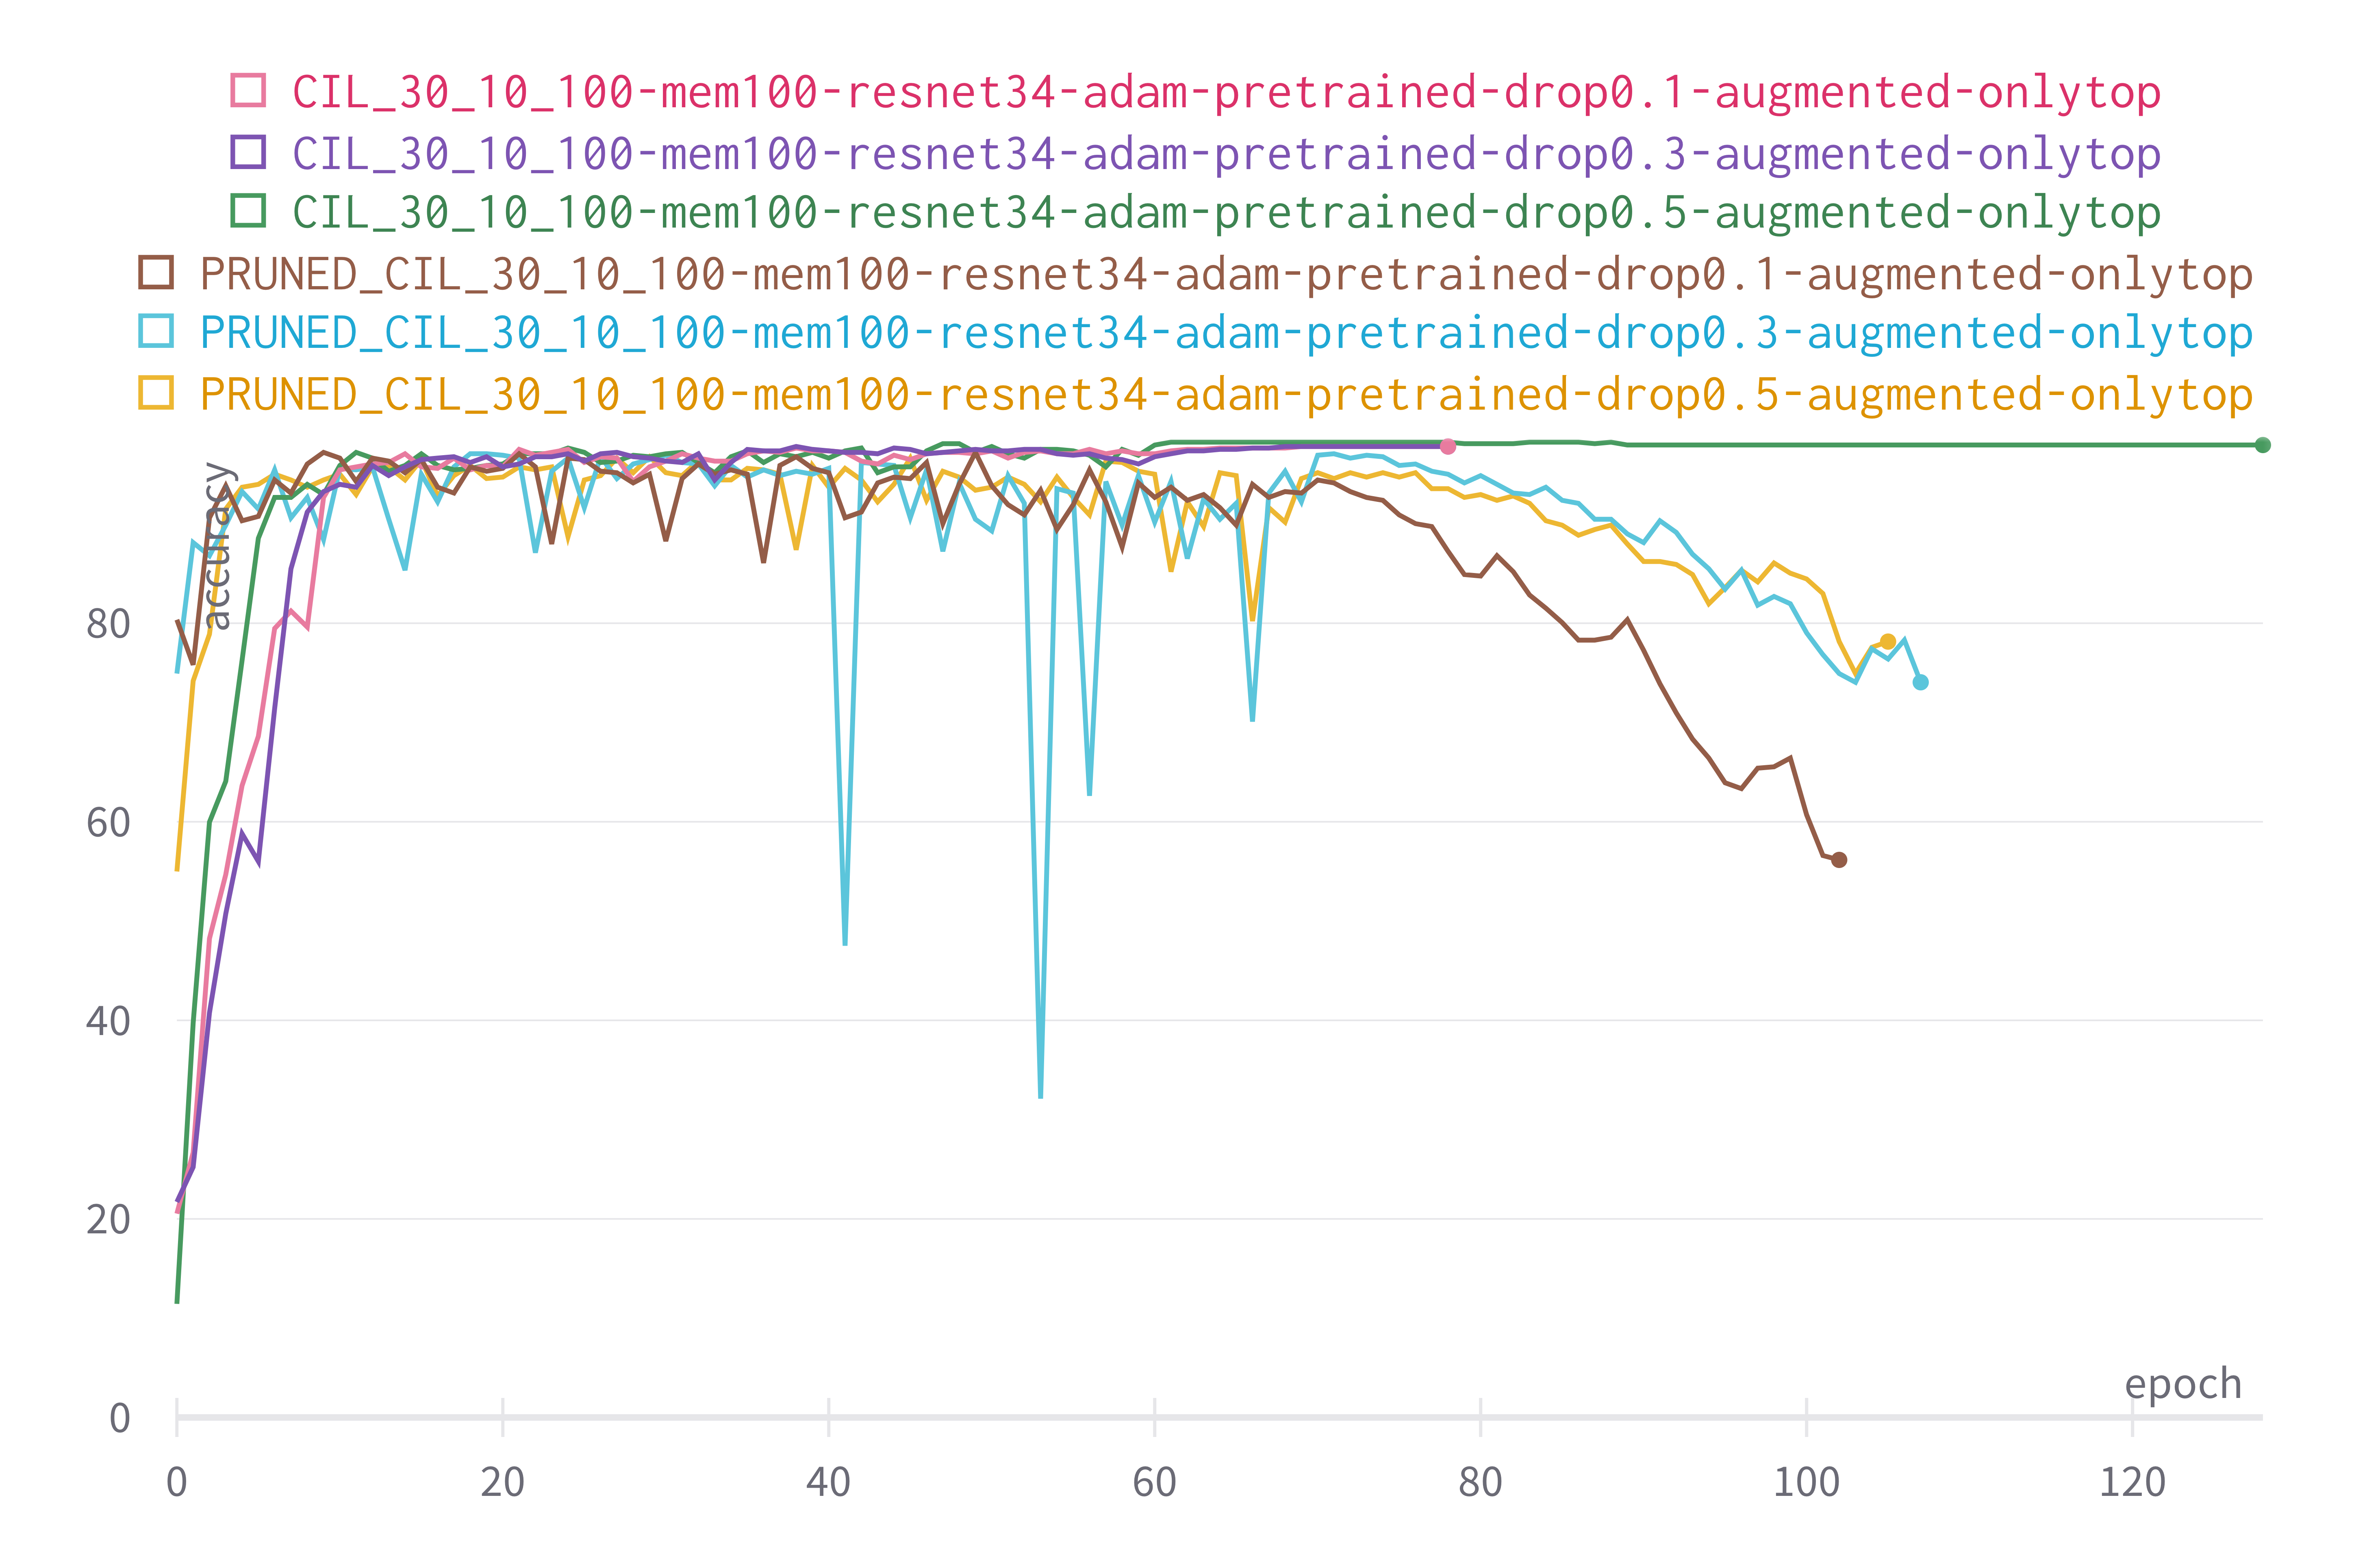
\includegraphics[width=0.50\textwidth]{images/exp/exp5-val_acc.png} }}%
	\subfloat[\centering Final loss]{{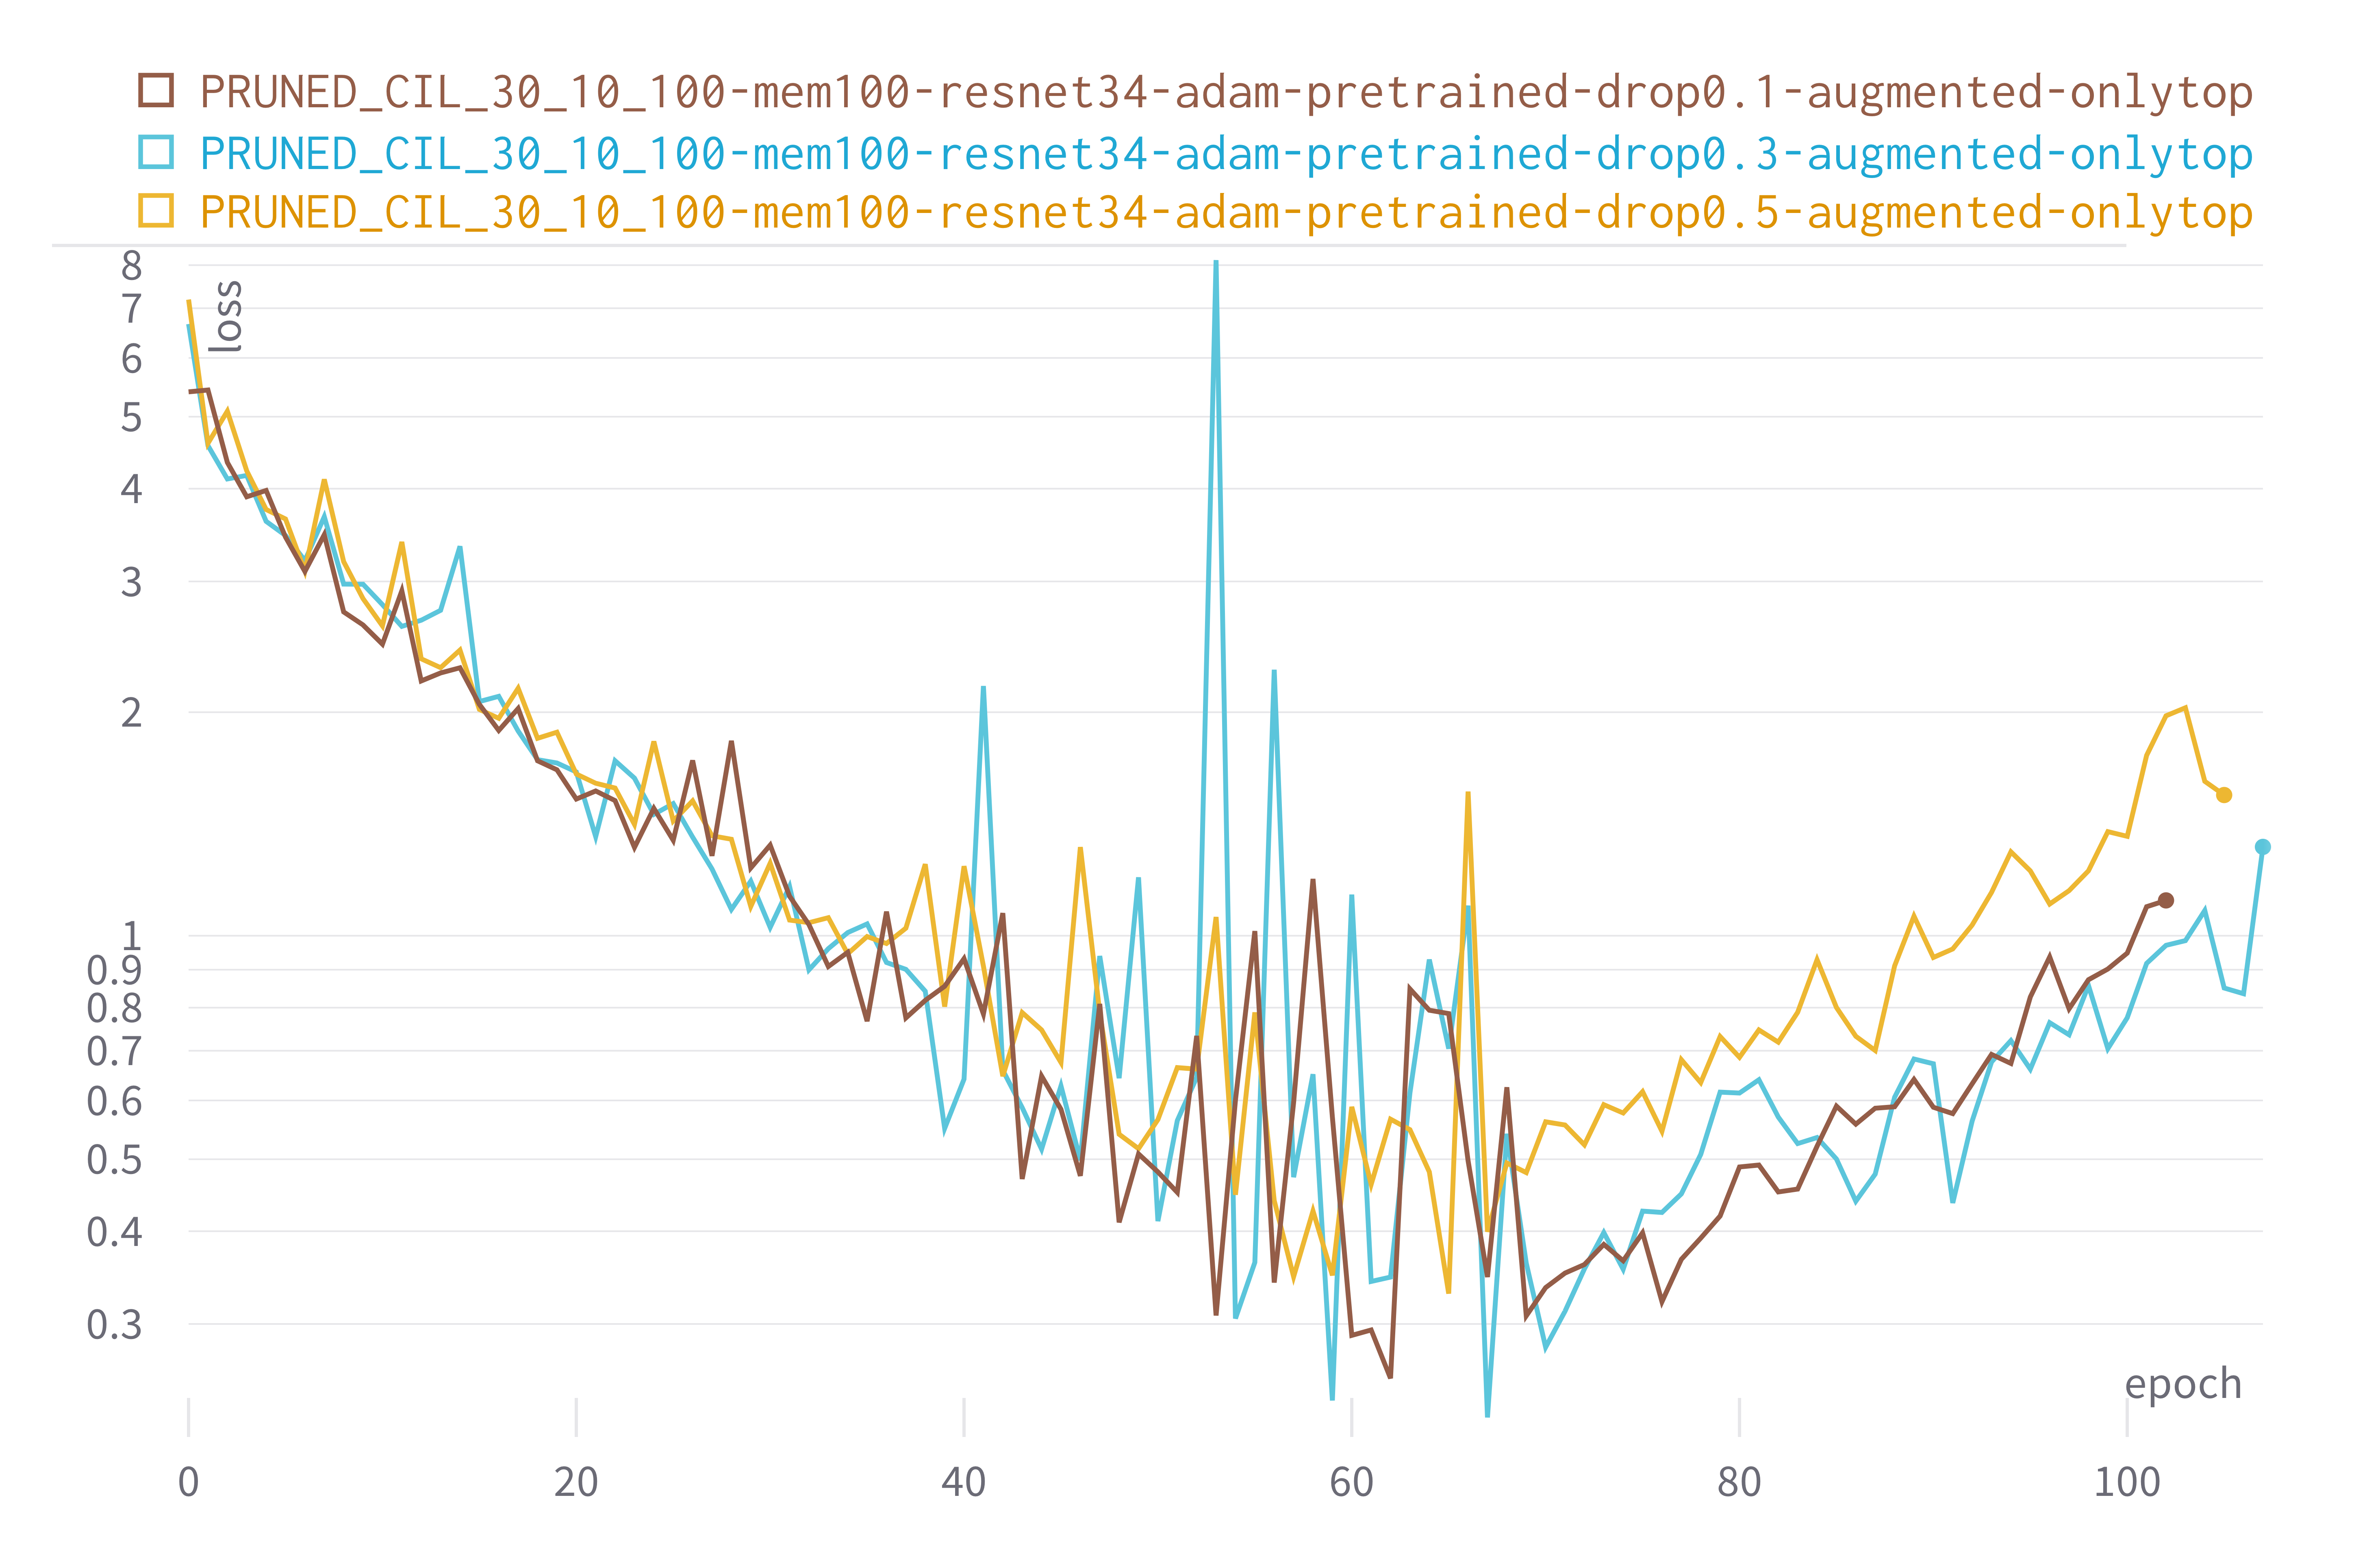
\includegraphics[width=0.50\textwidth]{images/exp/exp5-val_loss.png} }}%
    \qquad
	\subfloat[\centering Classification loss]{{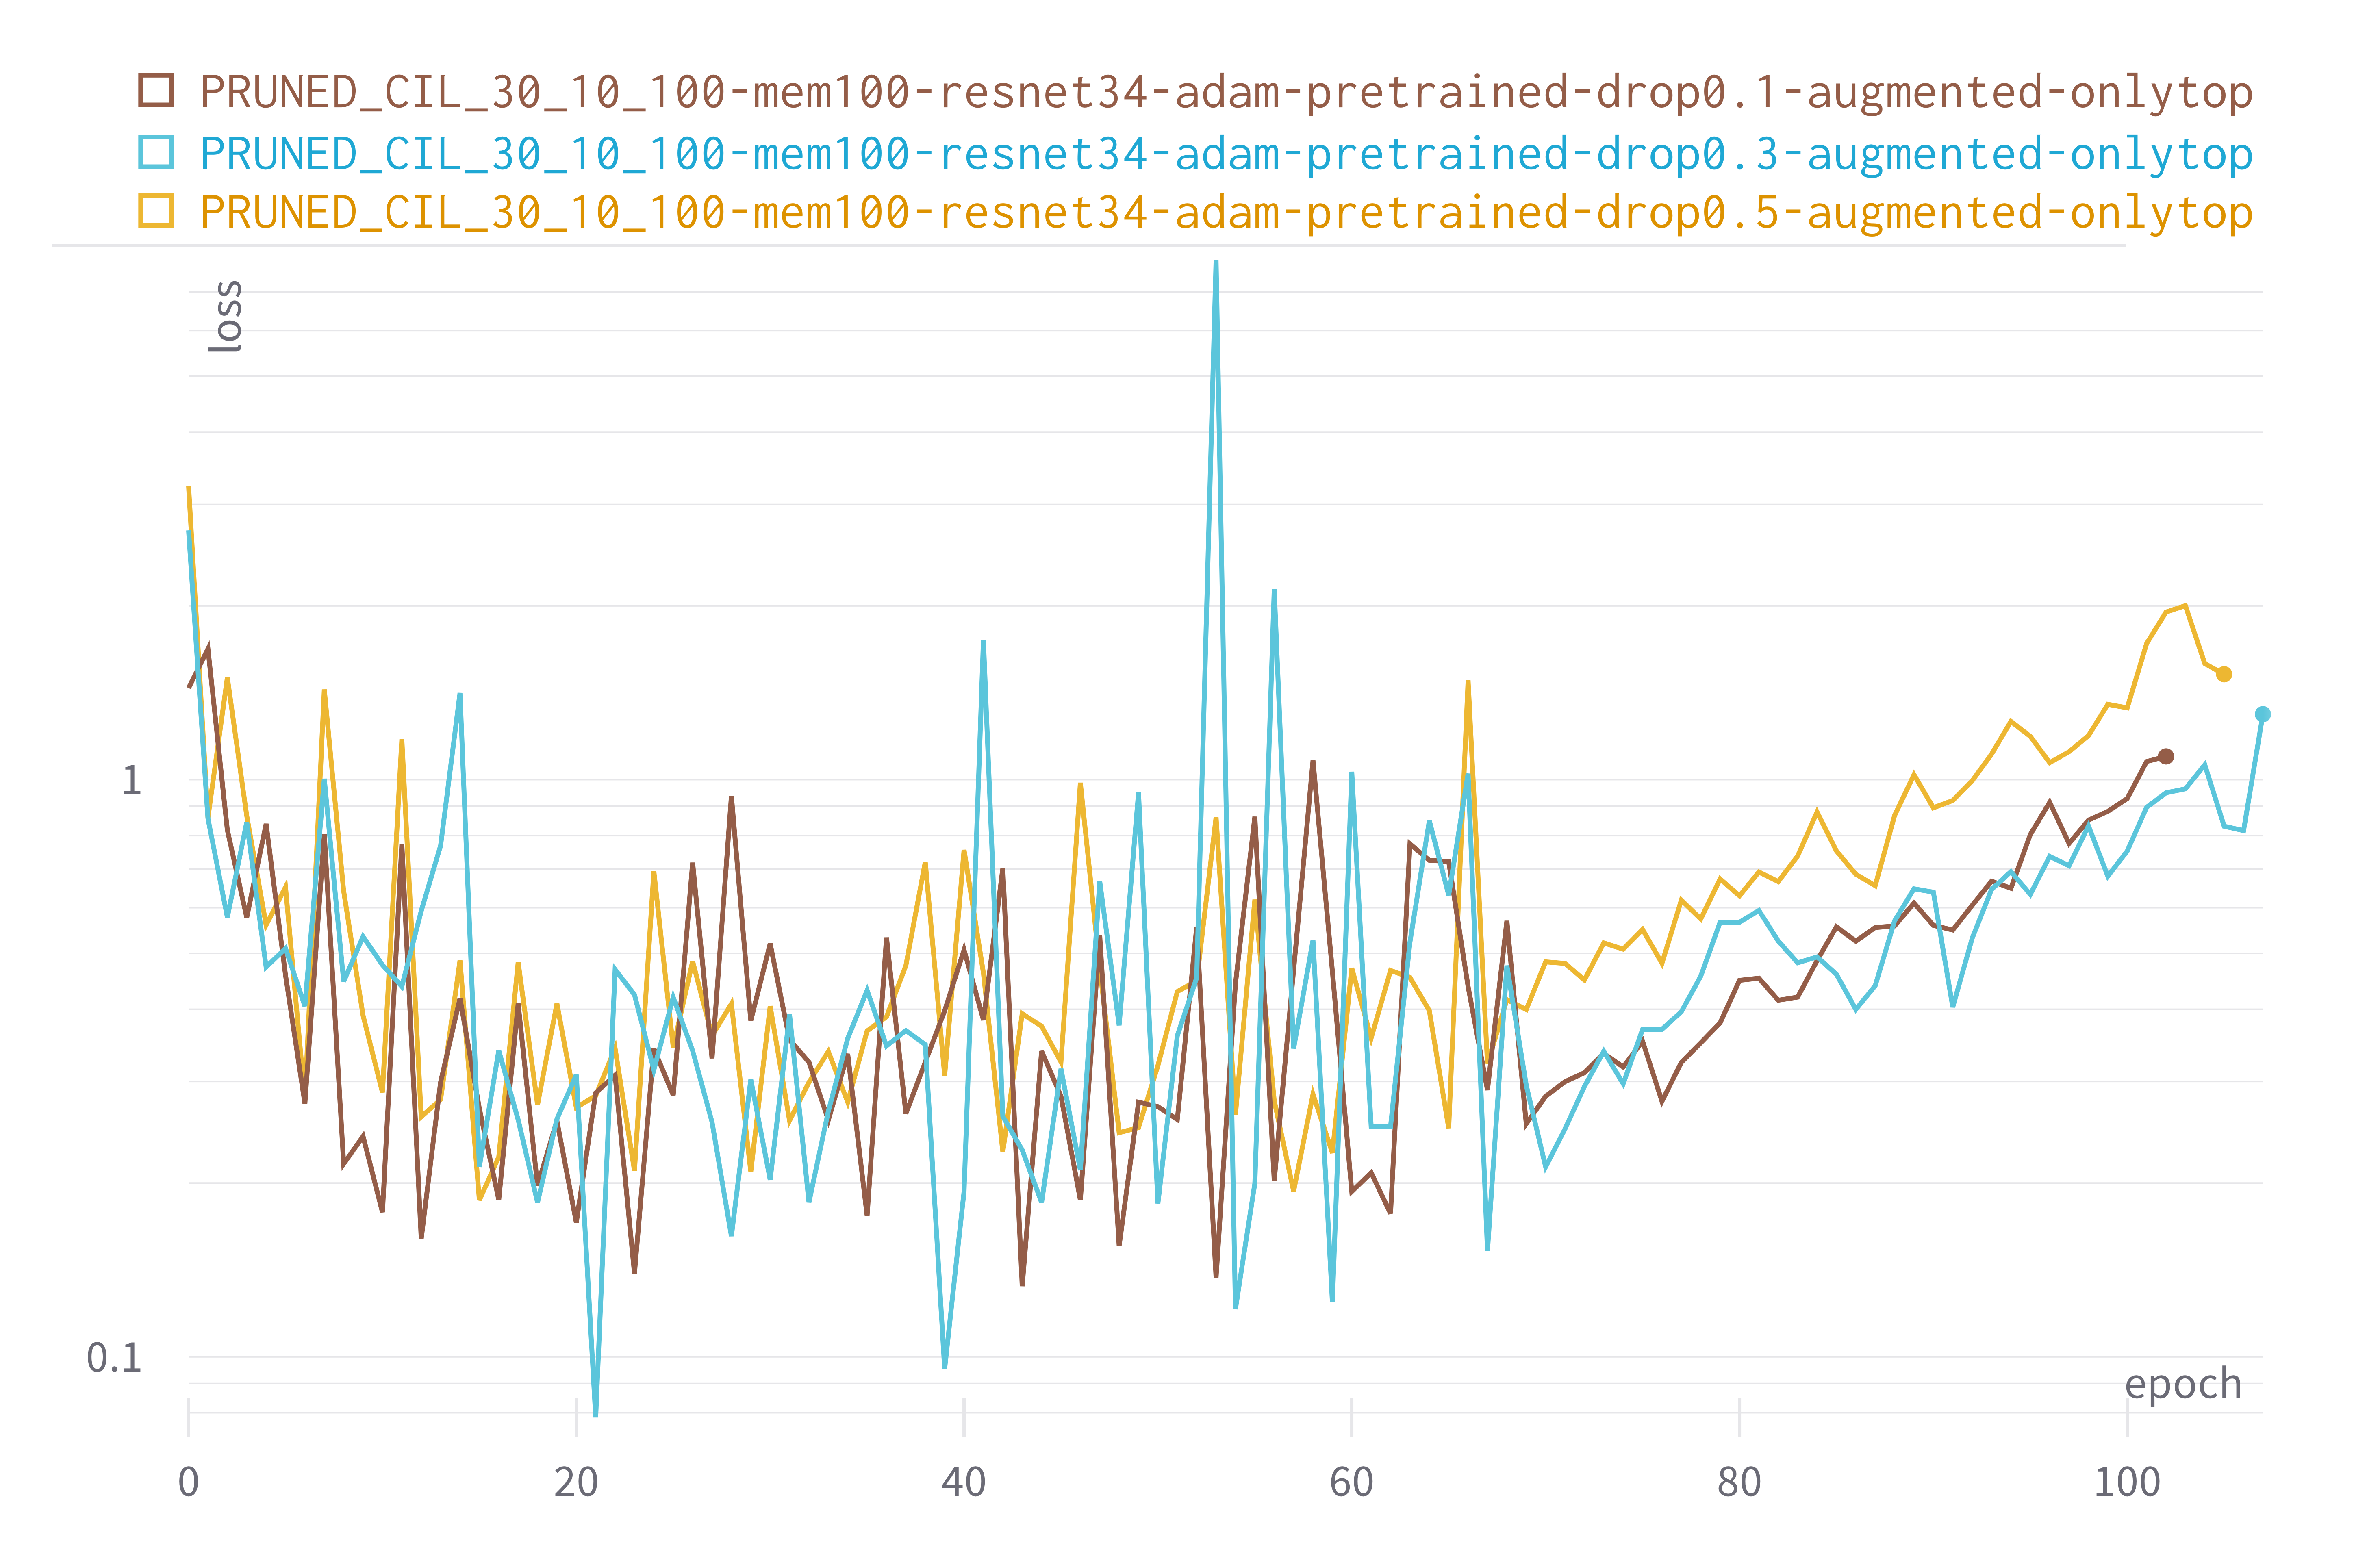
\includegraphics[width=0.50\textwidth]{images/exp/exp5-val_clf.png} }}%
	\subfloat[\centering Sparsity loss]{{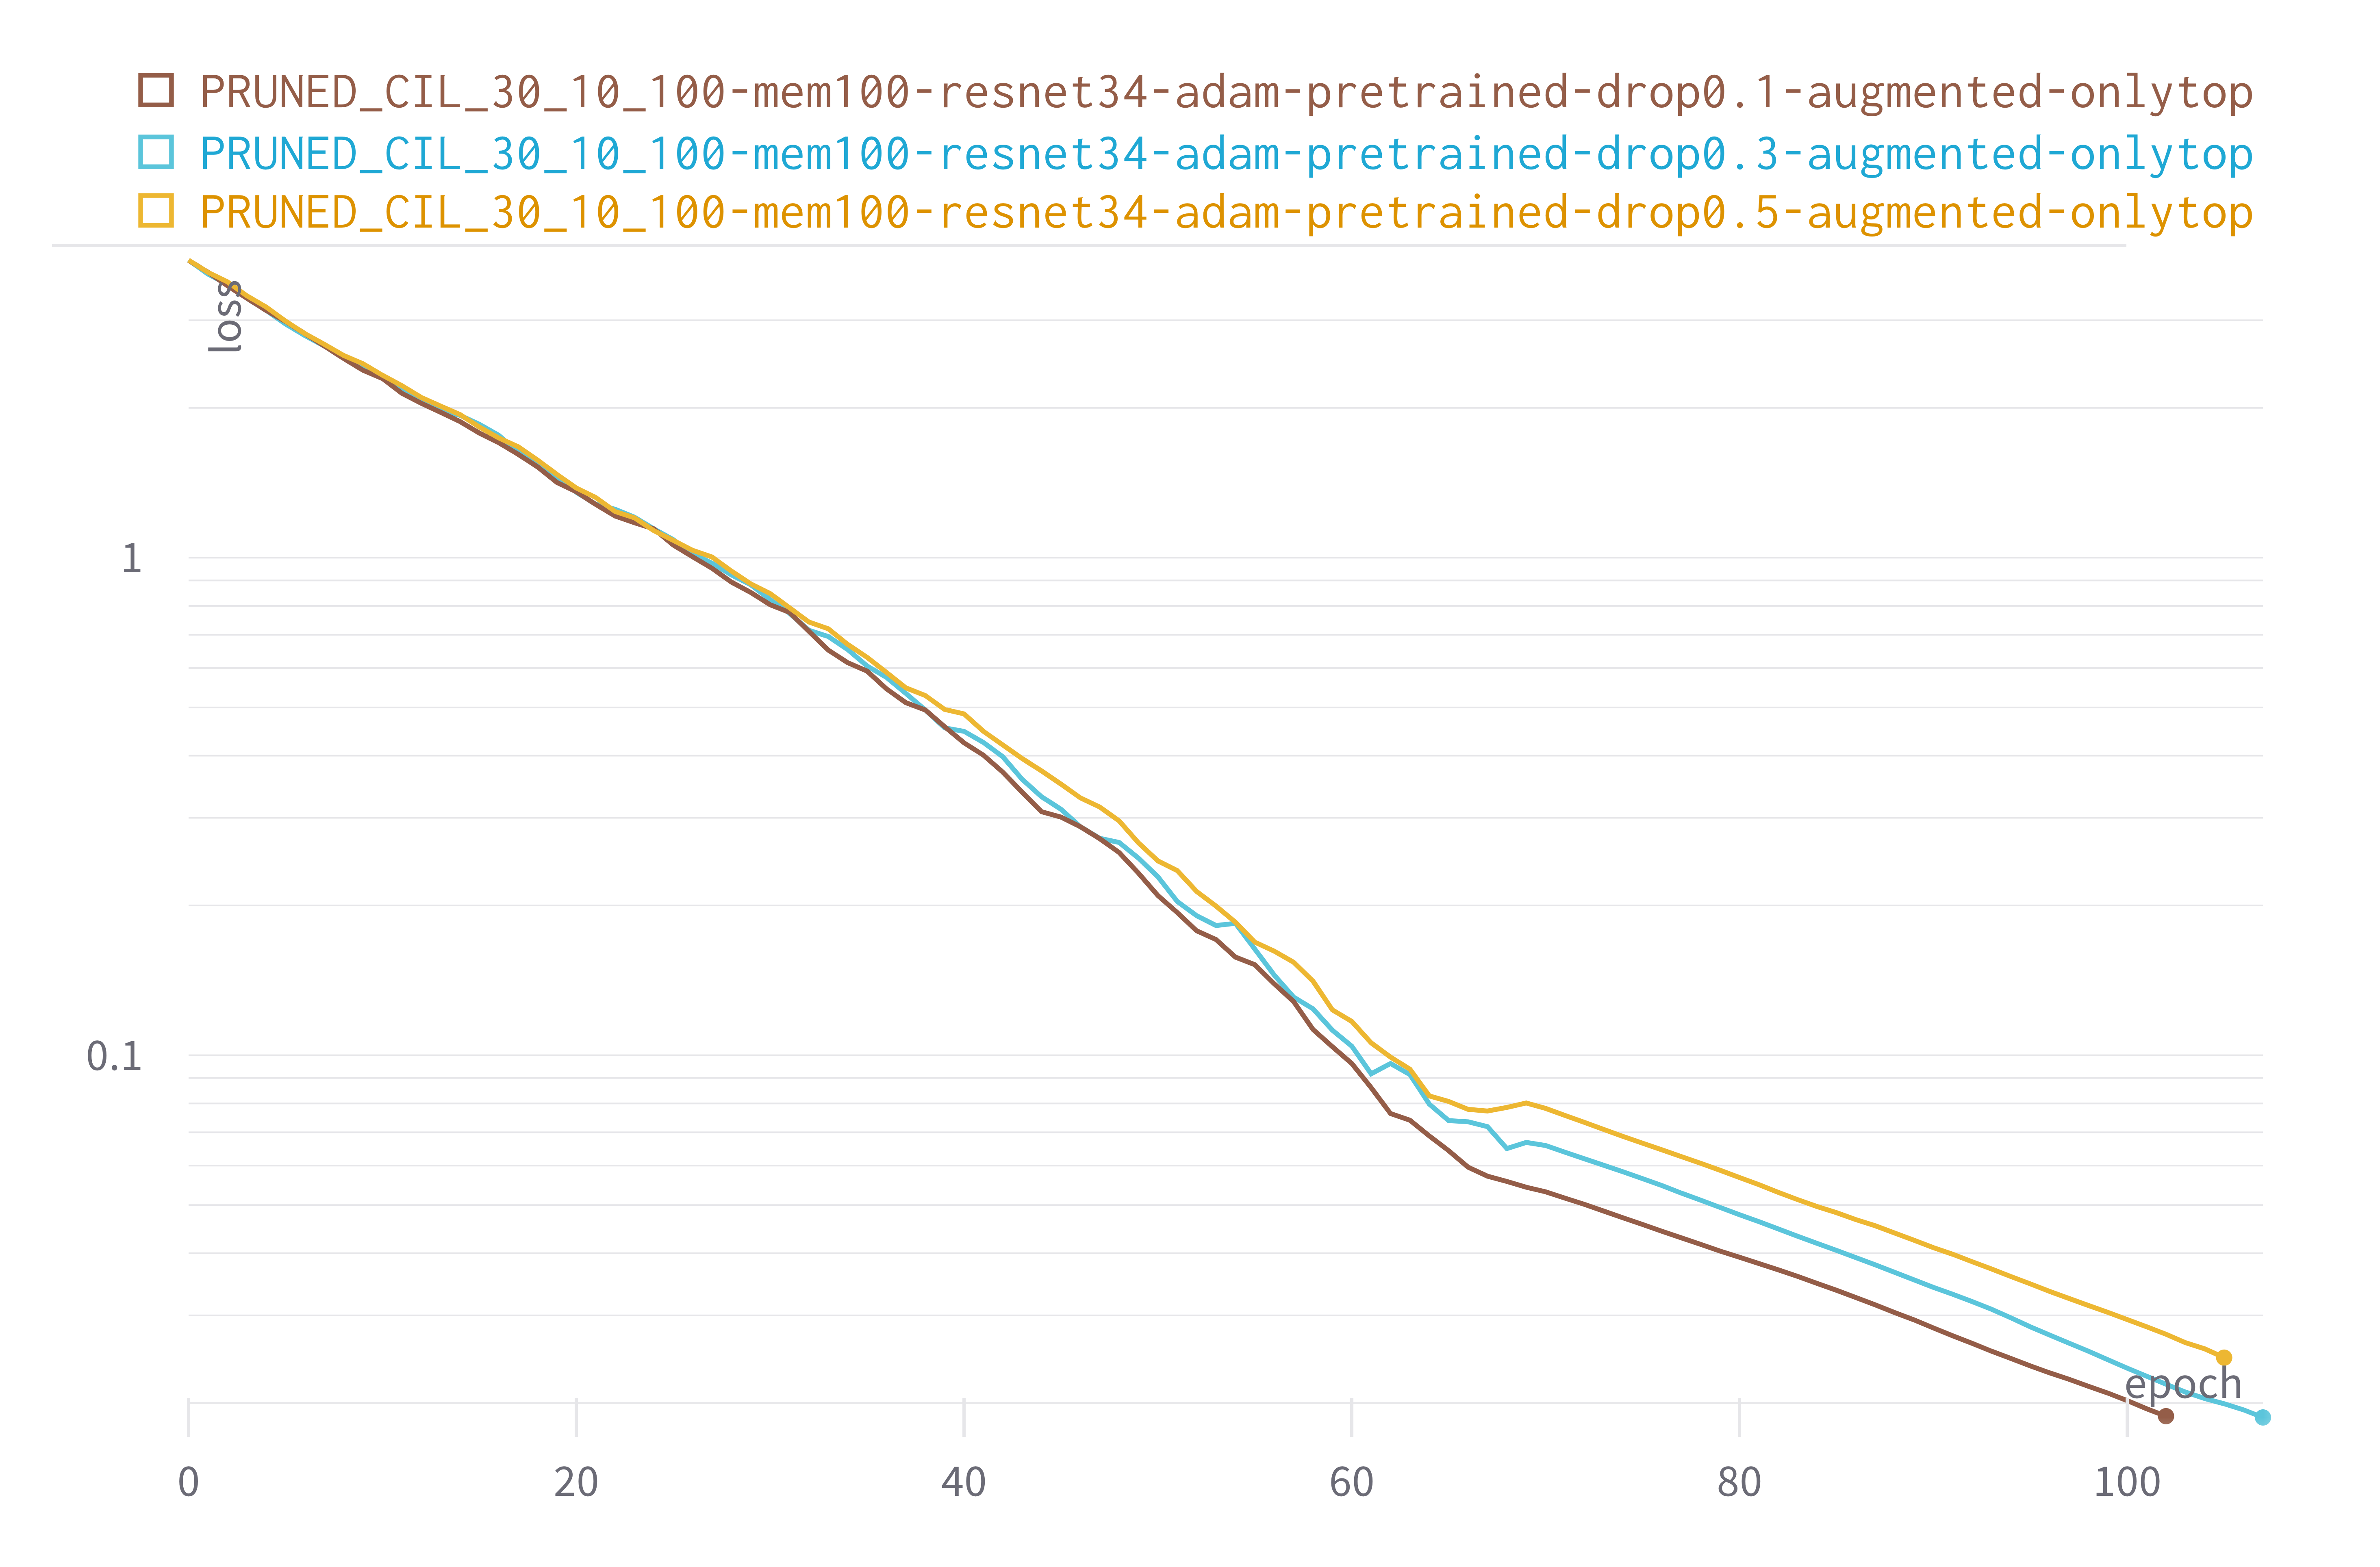
\includegraphics[width=0.50\textwidth]{images/exp/exp5-val_spars.png} }}%
	\caption{Training history of the pruned model calculated on the validation set at task 0.}%
	\label{fig:exp5-loss}%
\end{figure}


\subsection{2993 Classes}
\label{sec:whole_dataset_clf}

The following experiments test the scalability capabilities of the model by training it on 2993 classes, i.e. the entire dataset.

\subsubsection{Varying the memory size}
Another important factor for testing the scalability of the model is the number of examples stored for old classes.
Indeed, when many classes are introduced, it is necessary to limit the memory used to store old examples.
In this first section, models are trained in different configurations to consider various memory sizes used to store the examples of the old classes, in particular 50, 20 and 10 are the memory sizes taken into account.

The models are defined on the basis of the best results previously obtained from experiments on 100 classes: the architecture of each feature extractor is ResNet-34 pre-trained on ImageNet; the optimizer is Adam; regularization with a dropout layer is used as well as data augmentation. No pruning is performed initially.

The results of the experiments are shown in \autoref{fig:exp6} and \autoref{table:exp6}.
As we can see, the models scale quite well over the entire dataset, by comparison, considering the 100 classes setup shown in \autoref{table:exp5}, the drop in performance is only about 6\%.%, even though the examples stored in the setup of 2993 classes are 1/10th of what they were before.
Moreover, the results show that the greater the number of samples stored for incremental learning iterations, the better the overall accuracy.
The total number of examples stored by each model at task 8 is reported in \autoref{table:exp6-memsize}.

\begin{table}[H]
    \centering
    \centerline{
    \begin{tabular}{c|c|c|c|c}
        \hline
        \textbf{Model} &
        \textbf{Dropout} &
        \textbf{Mem.} &
        \textbf{Top-1} & 
        \textbf{Top-5} \\
        \textbf{name} &
        \textbf{rate} &
        \textbf{size} &
        \textbf{acc. (\%)} & 
        \textbf{acc. (\%)} \\
        \hline
        \hline
CIL\_2993-mem10-drop0.5-adam $\diamondsuit$ &0.1&10&87.2&92.19\\
CIL\_2993-mem20-drop0.5-adam&0.1&20&88.47&92.58\\
CIL\_2993-mem50-drop0.5-adam $\clubsuit$ &0.1&50&\textbf{89.22}&\textbf{92.97}\\
        \hline
    \end{tabular}}
    \caption{Performance of models at each incremental task trained on the entire dataset using different memory sizes.. Top-1 and top-5 accuracy at task 8.}
    \label{table:exp6}
\end{table}


\begin{table}[H]
    \centering
    \begin{tabular}{c|c|c}
        \hline
        \textbf{Model} &
        \textbf{Mem.} &
        \textbf{\# Total saved} \\
        \textbf{name} &
        \textbf{per class} &
        \textbf{examples (K)} \\
        \hline
        \hline
CIL\_2993-mem10-drop0.5-adam&10&102\\
CIL\_2993-mem20-drop0.5-adam&20&53\\
CIL\_2993-mem50-drop0.5-adam&50&29\\
        \hline
    \end{tabular}
    \caption{Number of total examples stored by each model at task 8.}
    \label{table:exp6-memsize}
\end{table}


\begin{figure}[H]
	\centering
	\subfloat[\centering Top-1 accuracy]{{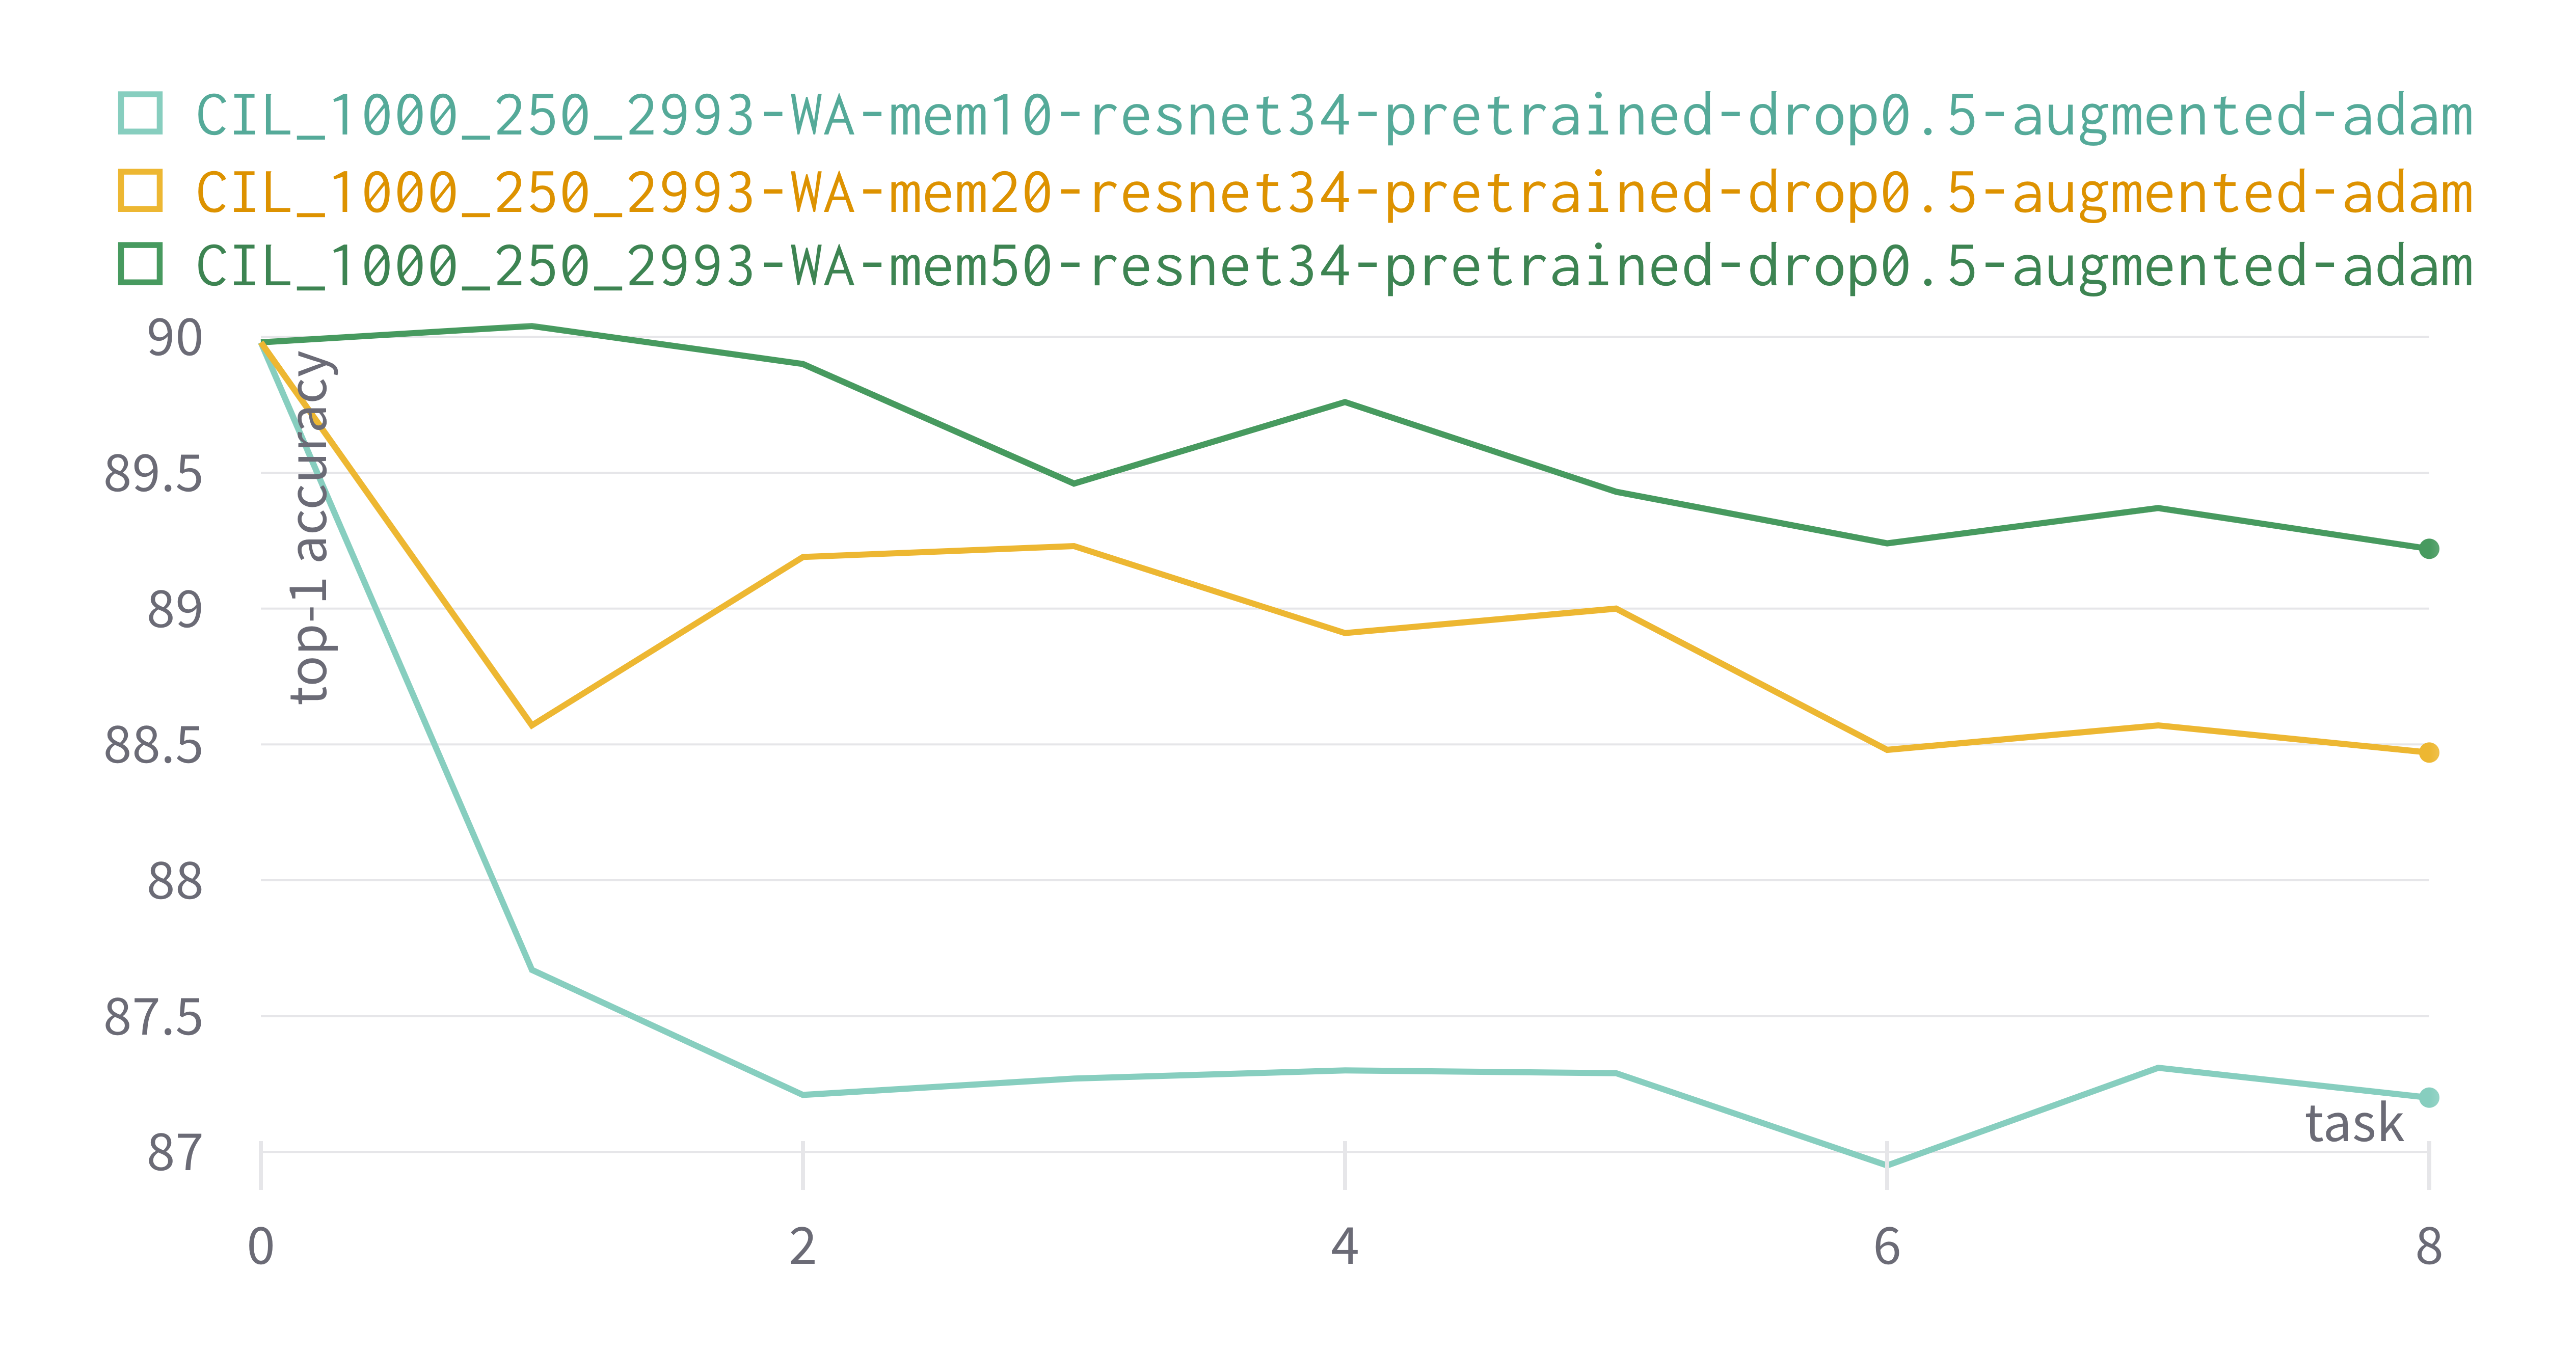
\includegraphics[width=0.50\textwidth]{images/exp/exp6-top1.png} }}%
    %\qquad
	\subfloat[\centering Top-5 accuracy]{{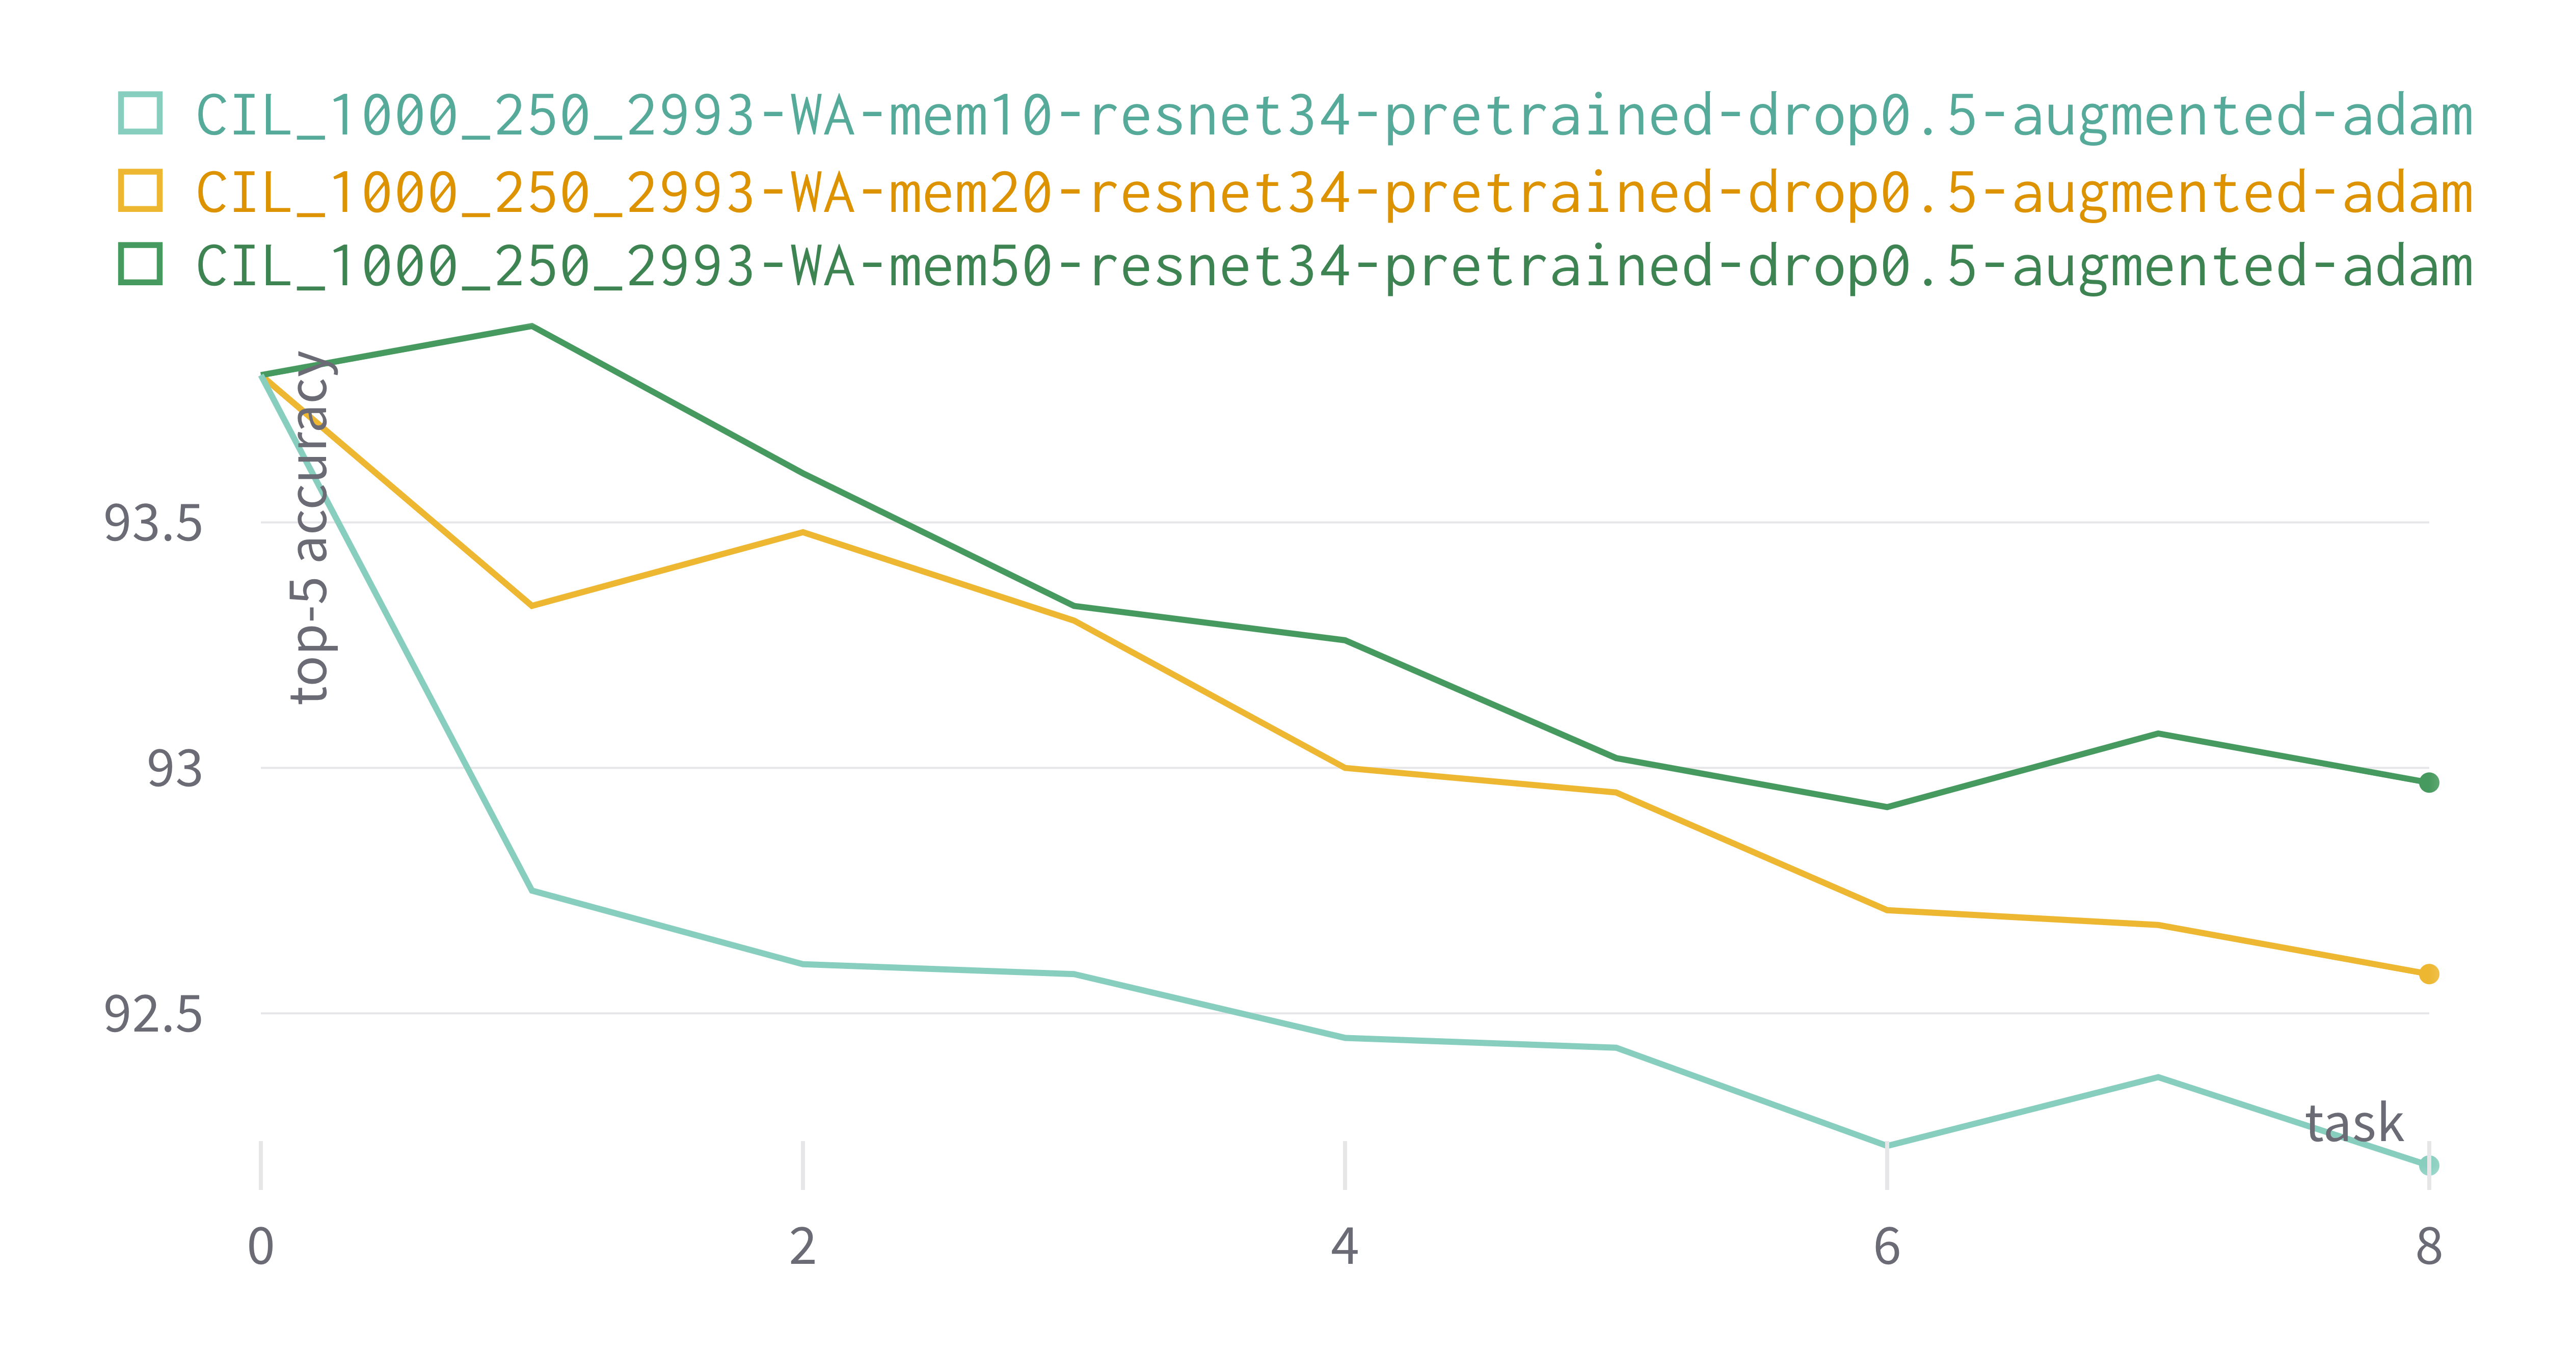
\includegraphics[width=0.50\textwidth]{images/exp/exp6-top5.png} }}%
	\caption{Performance of models at each incremental task trained on the entire dataset using different memory sizes.}%
	\label{fig:exp6}%
\end{figure}

%\newpage

\subsubsection{Type 3 baseline (2993 classes)}
As in the case of 100 classes, the performance of the CIL models is compared with the type 3 baseline (see \autoref{sec:method-baseline3}).
For this purpose, the baseline is trained considering the same dataset used to train the models in the previous section.
Note that in the case of the baseline, there is no need to use a memory for old classes, as the incremental learning setting does not hold.
 
The results of the comparison considering the top-1 accuracy between CIL models and baselines are shown in \todo{In tabella mancano dei risultati che andrò ad integrare nei prossimi giorni essendomi prenotato per usare il server}\autoref{table:baseline3-2993}.
As we can see, the top-1 accuracy of the best baseline is slightly better than that of the best CIL model, as in the 100 classes setup. The fact that the performance gap is so small proves that the DER algorithm is an effective approach for achieving CIL.

\begin{table}[H]
    \centering
    \centerline{
    \begin{tabular}{c|c|c|c}
        \hline
        \textbf{Model} &
        \textbf{Dropout} &
        \textbf{Mem.} &
        \textbf{Top-1}\\
        \textbf{name} &
        \textbf{rate} &
        \textbf{size} &
        \textbf{acc. (\%)} \\
        \hline
\hline
CIL\_2993-mem10-drop0.5-adam&0.1&10&87.2\\
CIL\_2993-mem20-drop0.5-adam&0.1&20&88.47\\
CIL\_2993-mem50-drop0.5-adam&0.1&50&89.22\\
\hline\
BASELINE\_3-2993classes-drop0.1&0.1&-&-\\
BASELINE\_3-2993classes-drop0.3&0.3&-&\textbf{91.92}\\
BASELINE\_3-2993classes-drop0.5&0.5&-&-\\
\hline 
    \end{tabular}}
    \caption{Top-1 accuracy of the CIL model and the type 3 baseline considering all 2993 classes of the test set.}
    \label{table:baseline3-2993}
\end{table}

%\newpage

\subsubsection{Pruning (2993 classes)}
\label{sec:pruning-entire}
Similar to the setup with 100 classes, the pruning strategy is tested for models trained on the entire dataset.
As we can see from \autoref{fig:exp7} and \autoref{table:exp7}, when pruning is used in combination with Weight Aligning (WA), performance drops dramatically.
Therefore, only for models using pruning, WA is disabled.

In contrast to the 100-class experiments, pruning now yields poor performance.
In fact, the drop in accuracy is considerable compared to those models without pruning.
Even considering the case where 50 samples are used for the pruning model, performance deteriorates by almost 20\%.

Regarding the number of parameters, even in the setup with 2993 classes, the model is significantly reduced in size.
However, as we can see from \autoref{table:exp7-params}, the pruning factor corresponds to approximately 3x compared to the 5x achieved in the previous setup.

In conclusion, the pruning strategy is not effective in the case of models trained on the entire dataset.
For this reason, the KD is used instead. The results of the experiments are shown in \autoref{sec:exp-kd}.

\begin{table}[H]
    \centering
    \begin{tabular}{c|c|c|c|c|c}
        \hline
        \textbf{Model} &
        \textbf{Mem.} &
        \textbf{WA} &
        \textbf{Pruning} &
        \textbf{Top-1} & 
        \textbf{Top-5} \\
        \textbf{name} &
        \textbf{size} &
        &
        &
        \textbf{acc. (\%)} & 
        \textbf{acc. (\%)} \\
        \hline
        \hline
UNPRUNED-WA-mem10-drop0.5&10&yes&no&87.2&92.19\\
UNPRUNED-WA-mem20-drop0.5&20&yes&no&88.47&92.58\\
UNPRUNED-WA-mem50-drop0.5&50&yes&no&\textbf{89.22}&\textbf{92.97}\\
\hline
PRUNED-noWA-mem10-drop0.3&10&no&yes&51.69&62.56\\
PRUNED-noWA-mem20-drop0.3&20&no&yes&63.2&73.97\\
PRUNED-noWA-mem50-drop0.3 $\spadesuit$&50&no&yes&70.37&81.85\\
\hline
PRUNED-WA-mem10-drop0.3&50&no&yes&7.6&10.67\\
\hline
\end{tabular}
\caption{Performance comparison between the pruned and un-pruned models. Top-1 and top-5 accuracy at task 8.}
    \label{table:exp7}
\end{table}


\begin{table}[H]
    \centering
    \begin{tabular}{c|c}
        \hline
        \textbf{Model} &
        \textbf{\#Params} \\
        \textbf{name} &
        \textbf{(M)} \\
        \hline
        \hline
UNPRUNED-CIL\_2993-WA-mem10-drop0.5&205\\
UNPRUNED-CIL\_2993-WA-mem20-drop0.5&205\\
UNPRUNED-CIL\_2993-WA-mem50-drop0.5&205\\
\hline
PRUNED-CIL\_2993-noWA-mem10-drop0.3&68.79\\
PRUNED-CIL\_2993-noWA-mem20-drop0.3&71.66\\
PRUNED-CIL\_2993-noWA-mem50-drop0.3&68.33\\
\hline
PRUNED-CIL\_2993-WA-mem10-drop0.3&70.69\\
        \hline
    \end{tabular}
	\caption{Number of model parameters at task 8.}%
    \label{table:exp7-params}
\end{table}

\begin{figure}[H]
	\centering
	\subfloat[\centering Top-1 accuracy]{{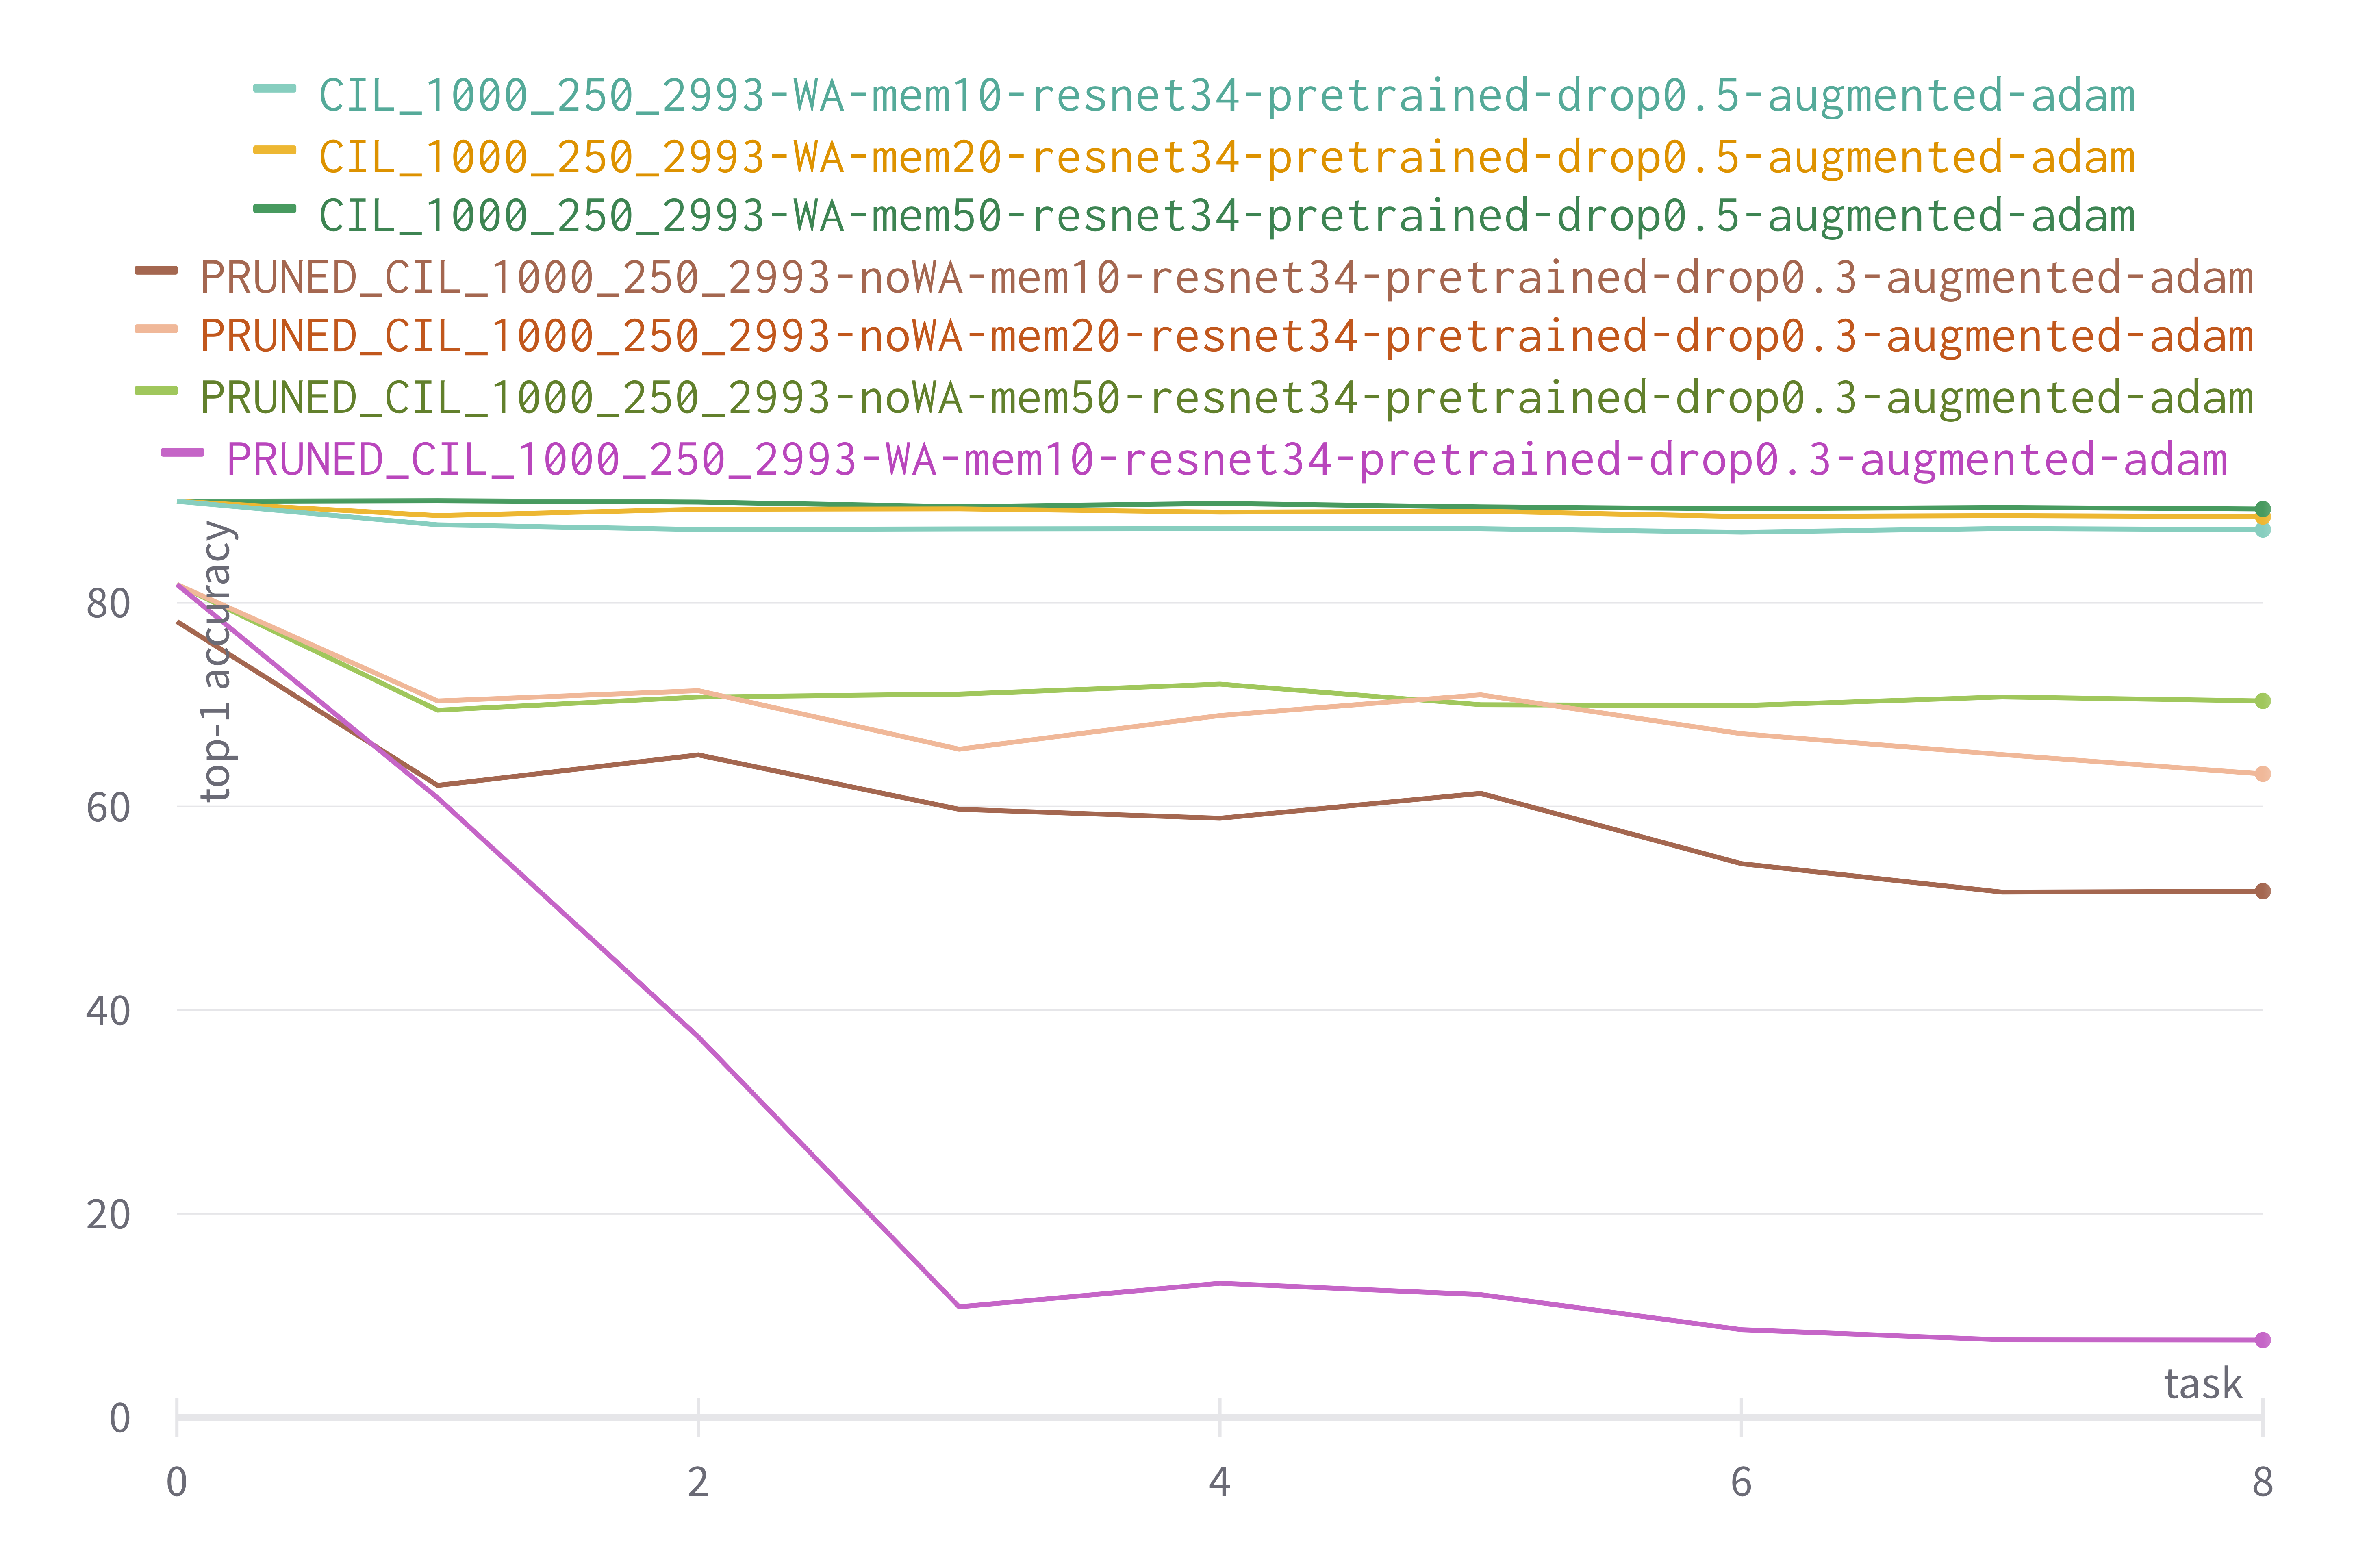
\includegraphics[width=0.50\textwidth]{images/exp/exp7-top1.png} }}%
    %\qquad
	\subfloat[\centering Top-5 accuracy]{{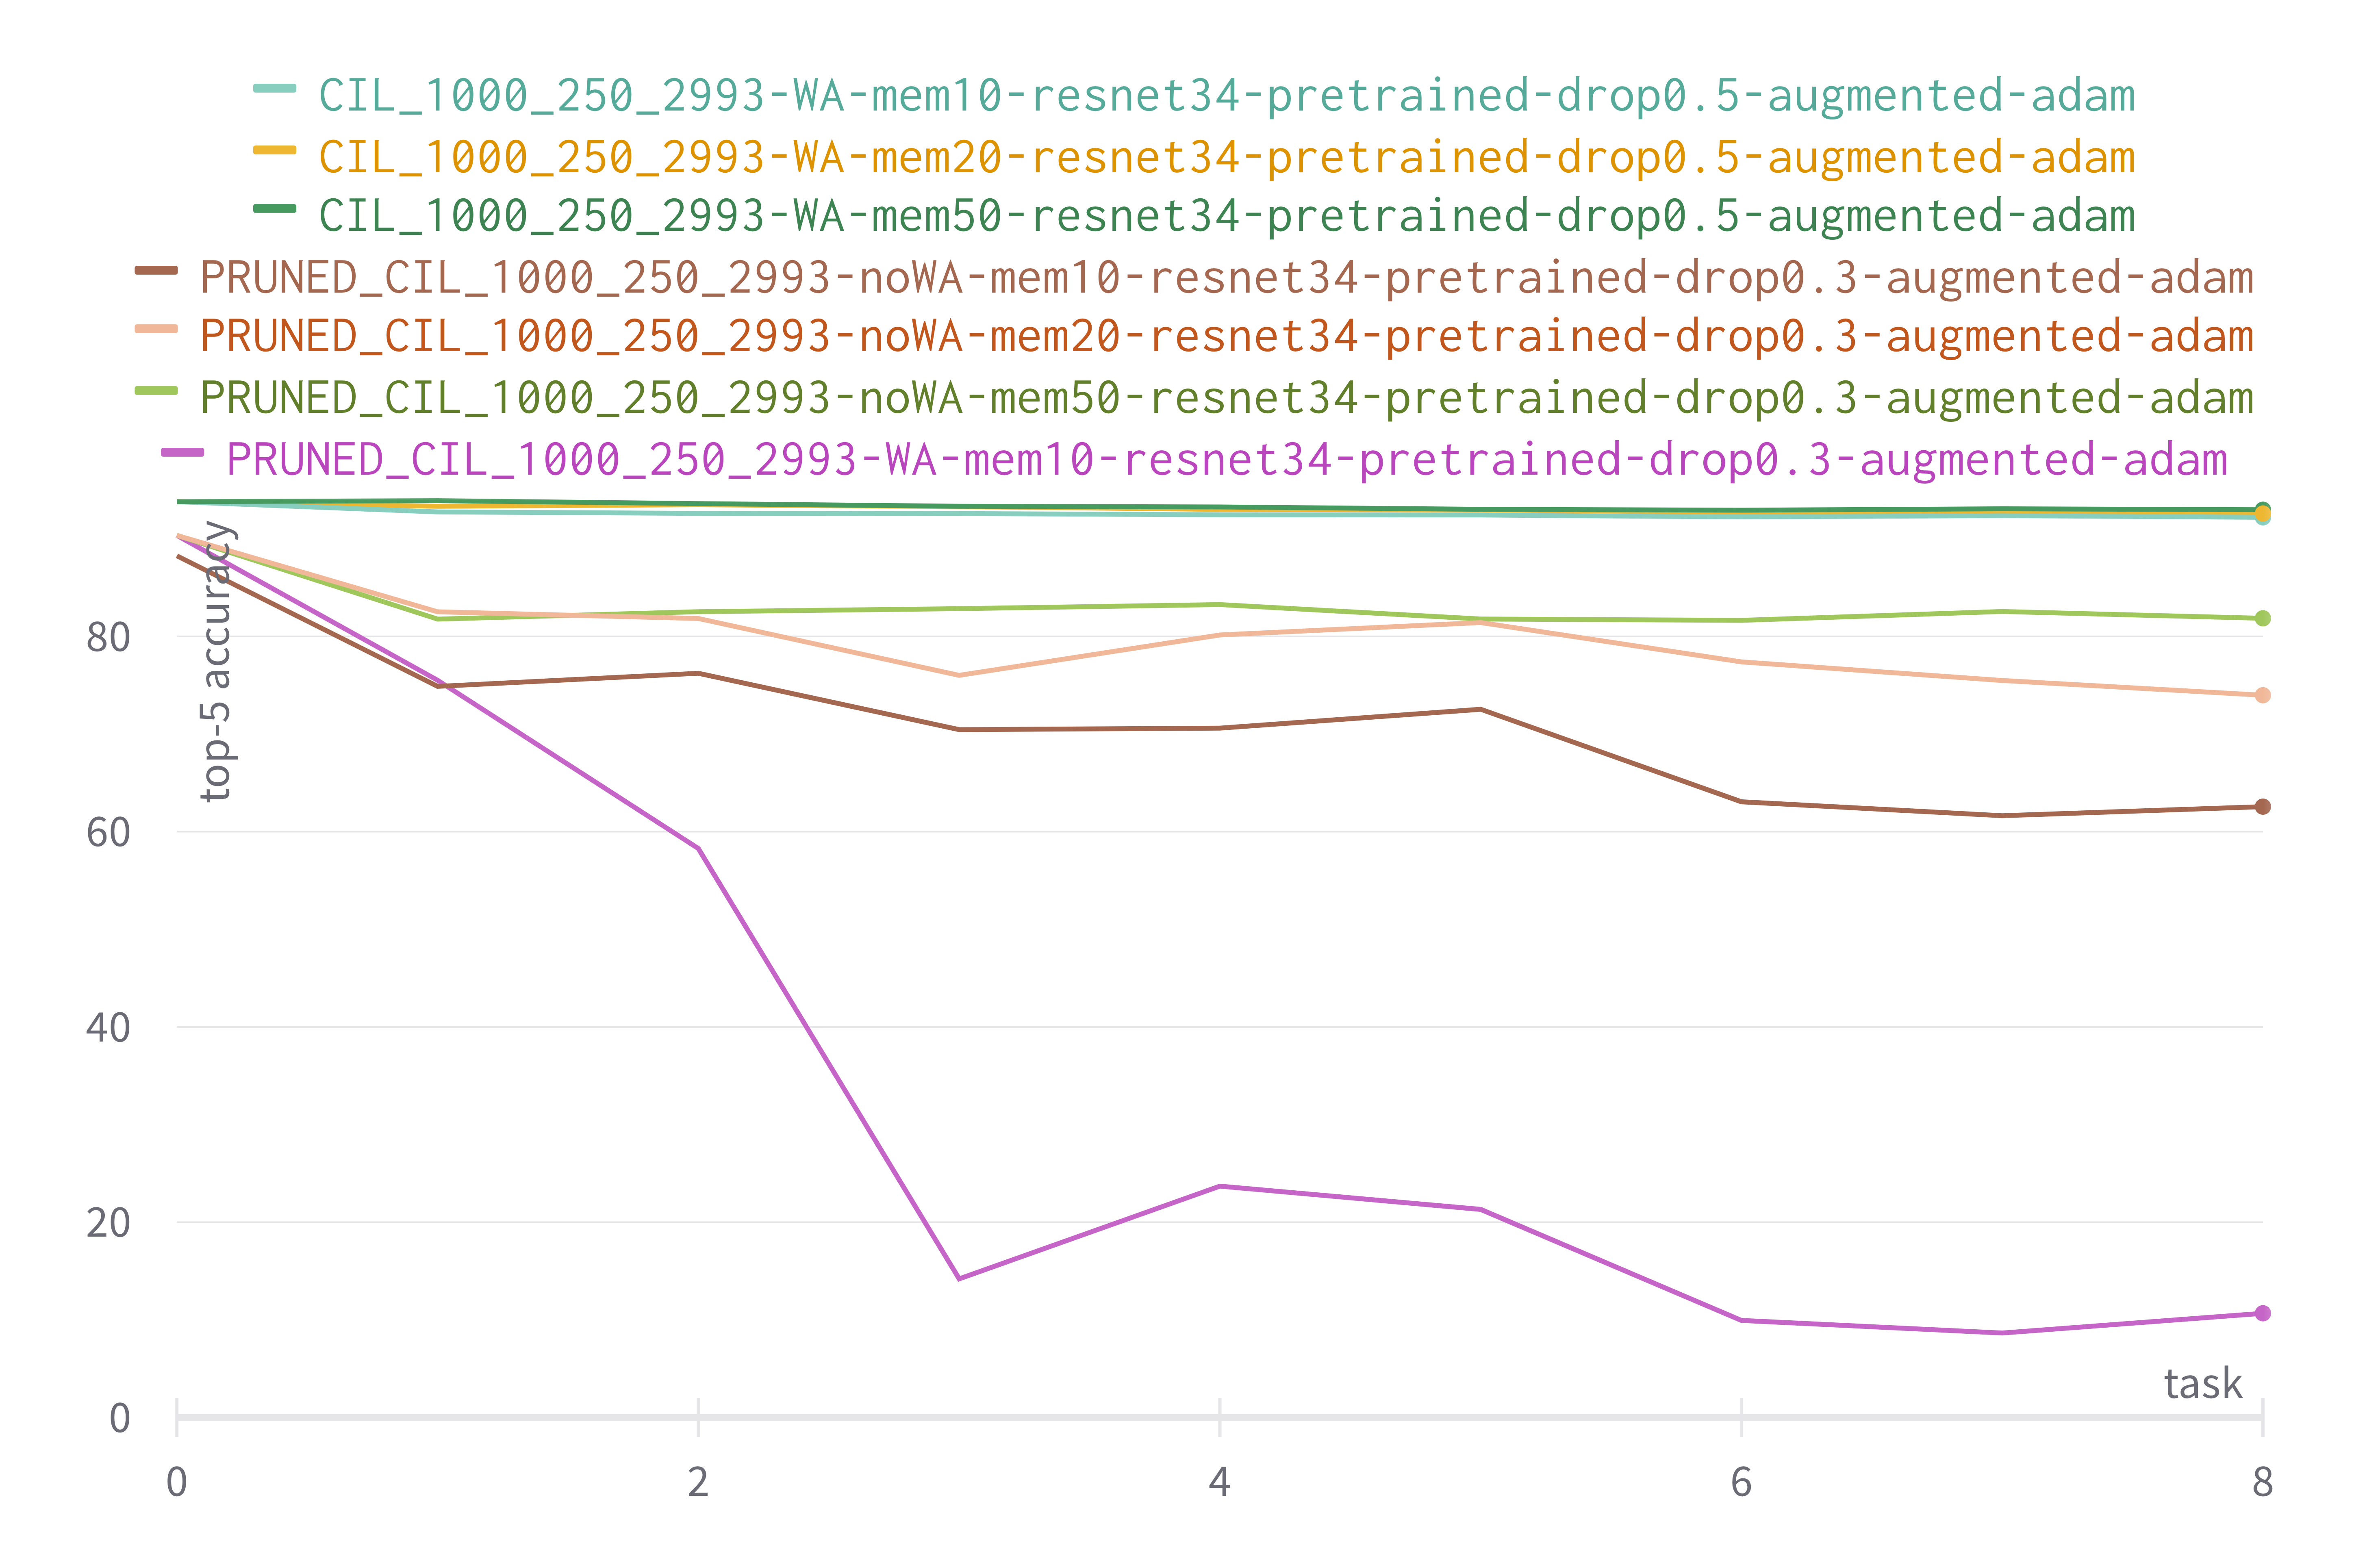
\includegraphics[width=0.50\textwidth]{images/exp/exp7-top5.png} }}%
	\caption{Performance comparison between the pruned and un-pruned model trained on the entire dataset considering the top-1 accuracy at each incremental task.}%
	\label{fig:exp7}
\end{figure}

%\newpage

%\subsubsection{Ablation study}

\section{Knowledge Distillation}
\label{sec:exp-kd}
To overcome the drastic drop in accuracy when using pruning on models trained on the entire dataset (see \autoref{sec:pruning-entire}), the KD is adopted as described in \autoref{sec:method-kd}.
During the KD, an un-pruned model is used as the teacher, while the student is a significantly smaller CNN. In the experiments presented in this section, ResNet-50 pretrained on ImageNet is used as the backbone for the student, with a dropout layer before the FC layer.

The KD is performed after the training of the teacher model.
Since the CIL classifier is trained using the DER algorithm and it requires the storage of a part of the examples of the old classes, in a real situation the KD can only be performed with those examples available as a result of the storage.
Therefore, in order to replicate a realistic situation, the student model is trained under the supervision of the teacher, but only the samples stored by the teacher are used as training data.

The result of the KD experiments are shown in \autoref{table:exp-kd}, where different models with varying memory sizes are used as teachers. As we can see, the number of samples used to train the student heavily affects the final performance.

Using 50 samples per class to train the student results in top-1 accuracy of 0.80\%, i.e. a decrease of 9\% compared to the teacher model.
Although this drop in performance is rather large, it is important to consider the number of parameters: all teacher models have 205 million parameters, while the final student models have 30 million parameters (the number of ResNet-50 parameters).
Therefore, even though the accuracy decreases, the number of parameters is reduced by almost 7 times.

The KD outperforms the pruning method (see \autoref{table:exp7} and \autoref{table:exp7-params}), increasing top-1 accuracy from 70.37\% to 80.0\% and the compression factor from 3x to 7x.

\begin{table}[H]
    \centering
    \begin{tabular}{c|c|c|c|c}
        \hline
        \textbf{Teacher} &
        \textbf{Student} &
        \textbf{Mem.} &
        \textbf{Student} &
        \textbf{Top-1} \\
        \textbf{model} &
        \textbf{model} &
        \textbf{size} &
        \textbf{dropout rate} &
        \textbf{acc. (\%)} \\
        \hline
        \hline
UNPRUNED-WA-mem10-drop0.5&ResNet-50&10&0.1&62.42\\
UNPRUNED-WA-mem50-drop0.5&ResNet-50&10&0.3&69.09\\
UNPRUNED-WA-mem50-drop0.5 $\heartsuit$&ResNet-50&50&0.3&\textbf{80.0}\\
\hline
\end{tabular}
\caption{Top-1 accuracy of the students trained using the KD. The student column refers to the backbone of the student model.}
    \label{table:exp-kd}
\end{table}


\section{Logo detector}
\label{sec:exp-det}
This section describes experiments designed to evaluate the class-agnostic logo detector introduced in \autoref{sec:method-roi}.
The CIL classifier is trained starting from the cropped regions, while the detector predicts the bounding boxes using the entire image as input.
Since an image can contain several logos, there is a need to train the detector using the same training, validation and testing sets used by the CIL classifier.
This is done by considering training labels for the detector only if the bounding box corresponds to a ROI used as a training example for the CIL classifier, otherwise the bounding box is used in the validation or test set, depending on the split used for the classifier.
This process is shown in \autoref{fig:detector-split-dataset}.
In this way, an unbiased evaluation of both the detector and the CIL classifier is achieved.

\begin{figure}[H]
	\centering
    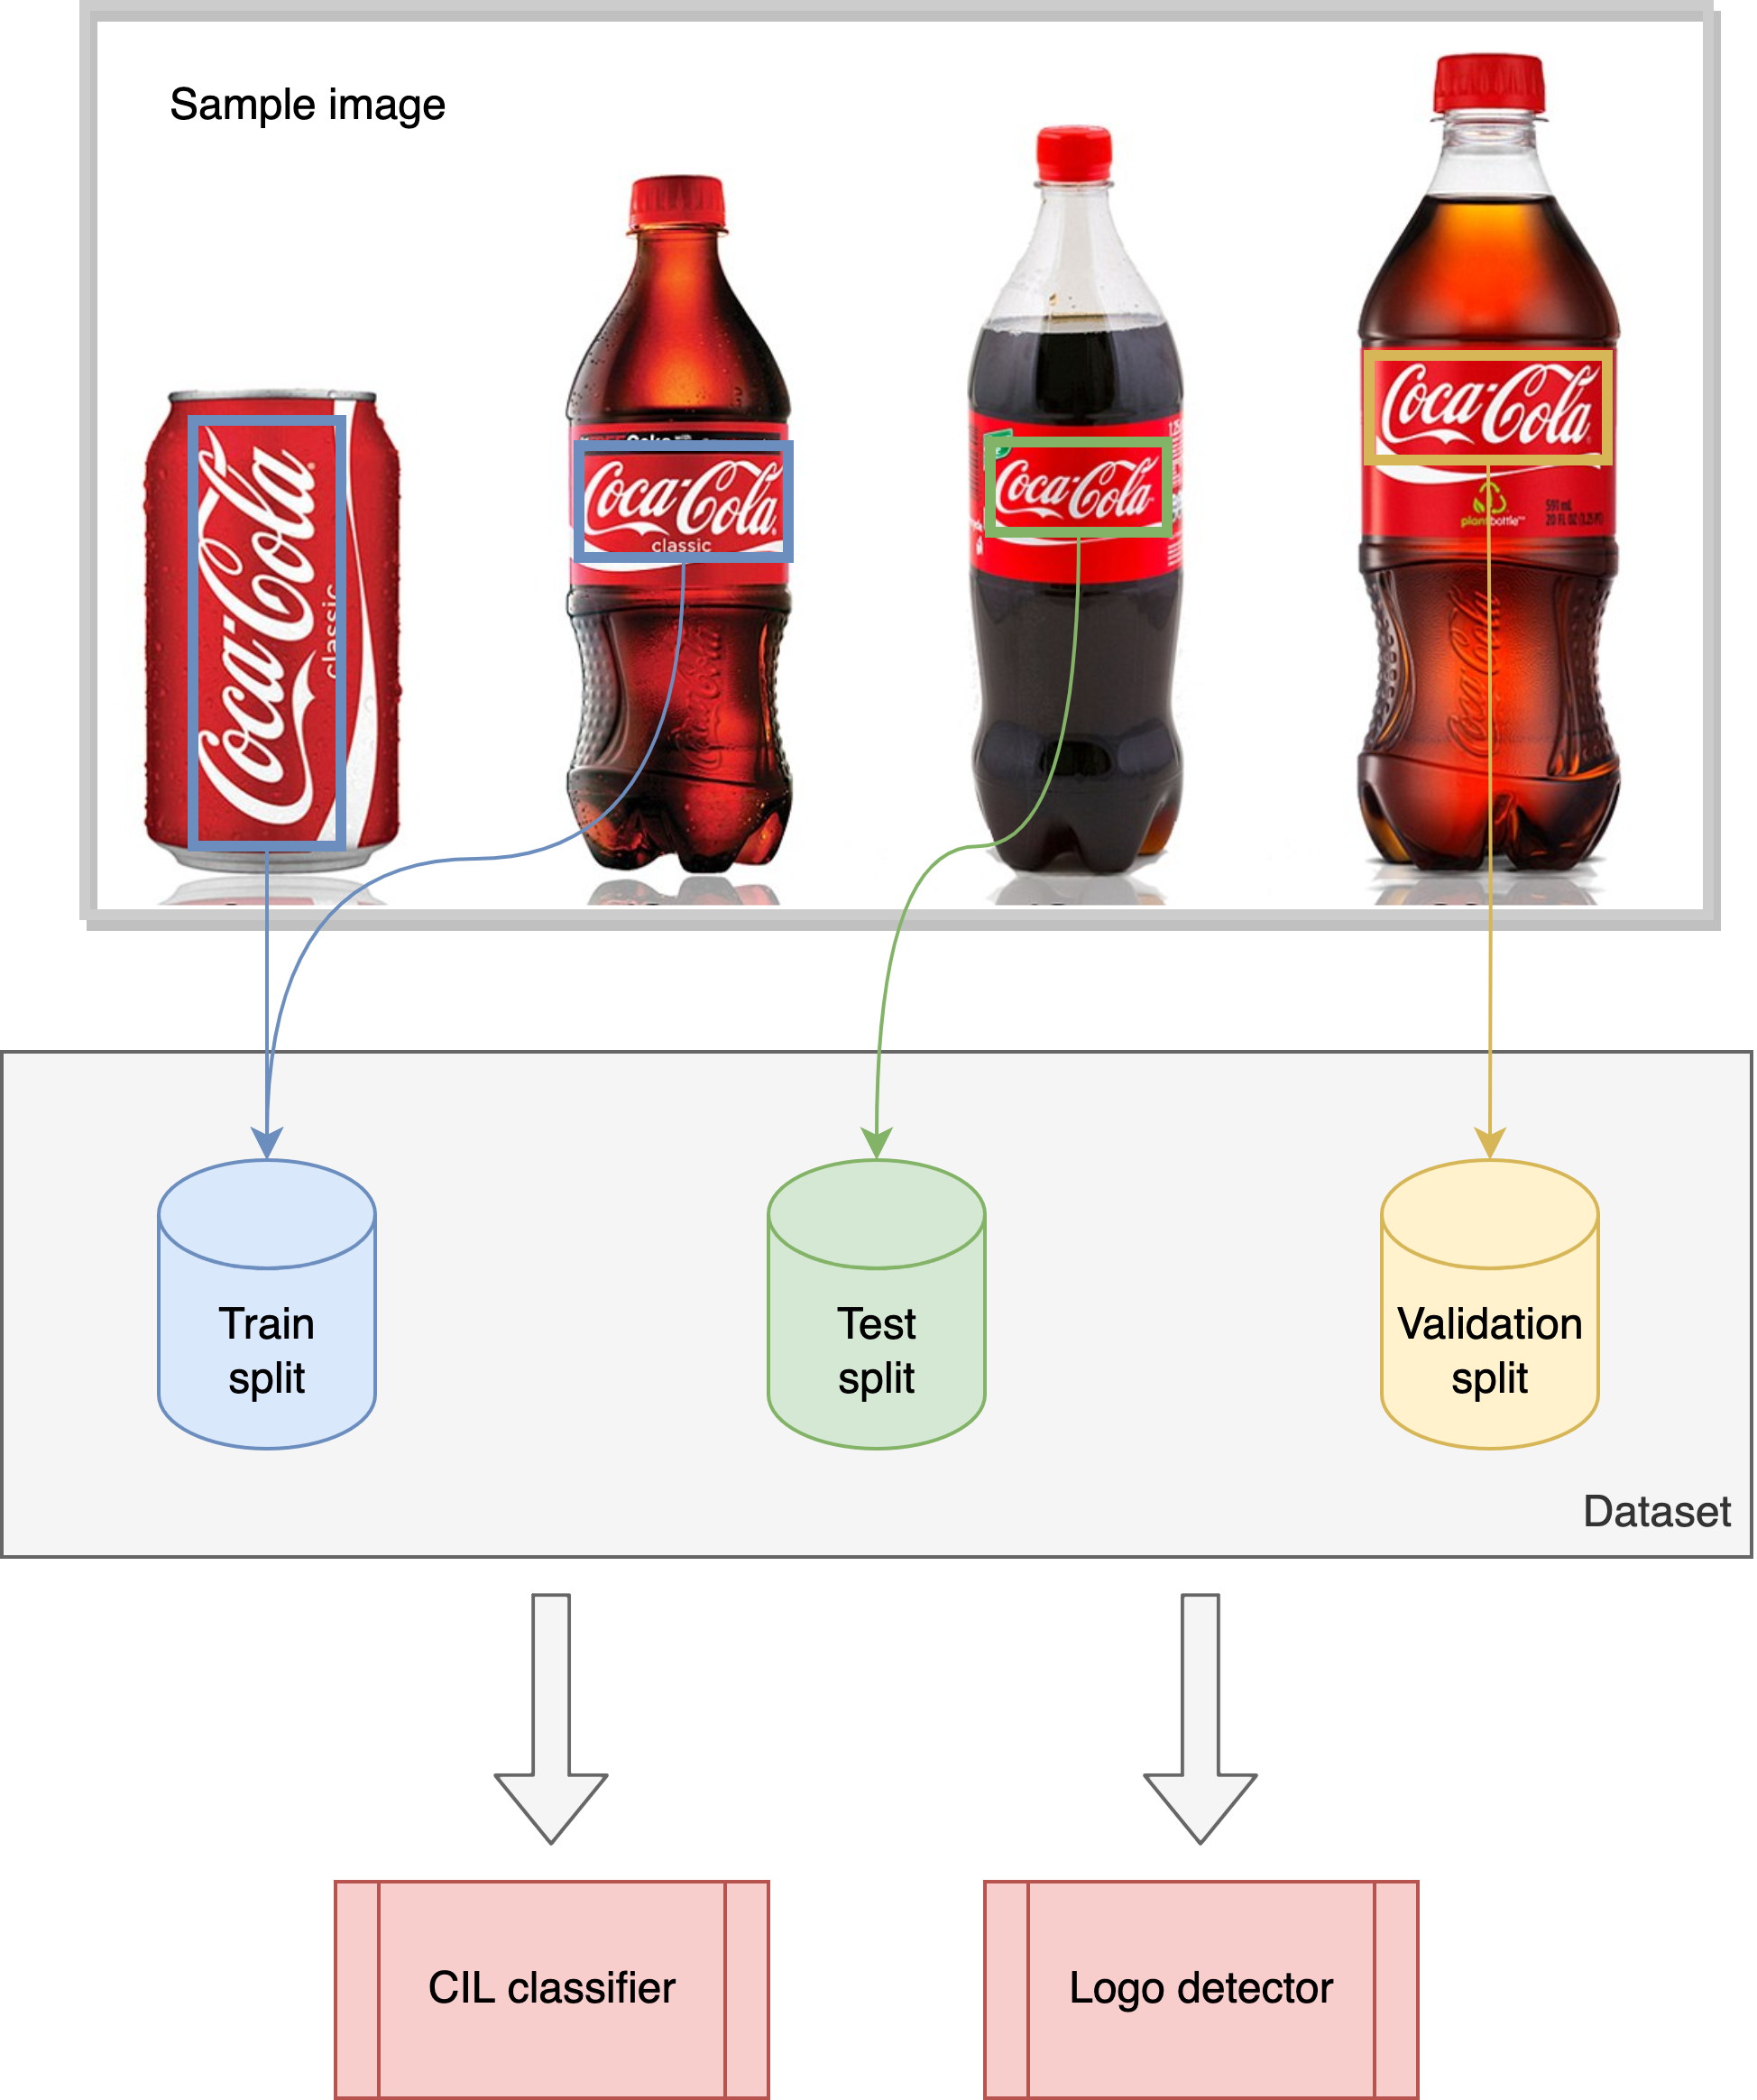
\includegraphics[width=0.5\textwidth]{images/logos-split.drawio.png}
	\caption{Training, validation and test sets used for the detector built on the splits used to train the CIL classifier.}%
	\label{fig:detector-split-dataset}%
\end{figure}

\subsection{Metrics}
Mean Average Precision (mAP) metric is a metric used to evaluate object detection models. This metric is based on: Intersection over Union (IoU), Recall, Precision.

\subsubsection{Intersection over Union}
Given a ground-truth bounding box $box_{gt}$ and a detected bounding box $box_{pred}$, as shown in \autoref{fig:iou}, the IoU is computed as the ratio of the overlap and union areas:
\begin{equation}
    \text{IoU} = \frac{box_{gt} \cap box_{pred}}{box_{gt} \cup box_{pred}} 
\end{equation}
A prediction is considered correct if IoU $ \geq \tau$, where $\tau$ is a threshold (a typical value for $\tau$ is $0.5$).

\begin{figure}[H]
	\centering
    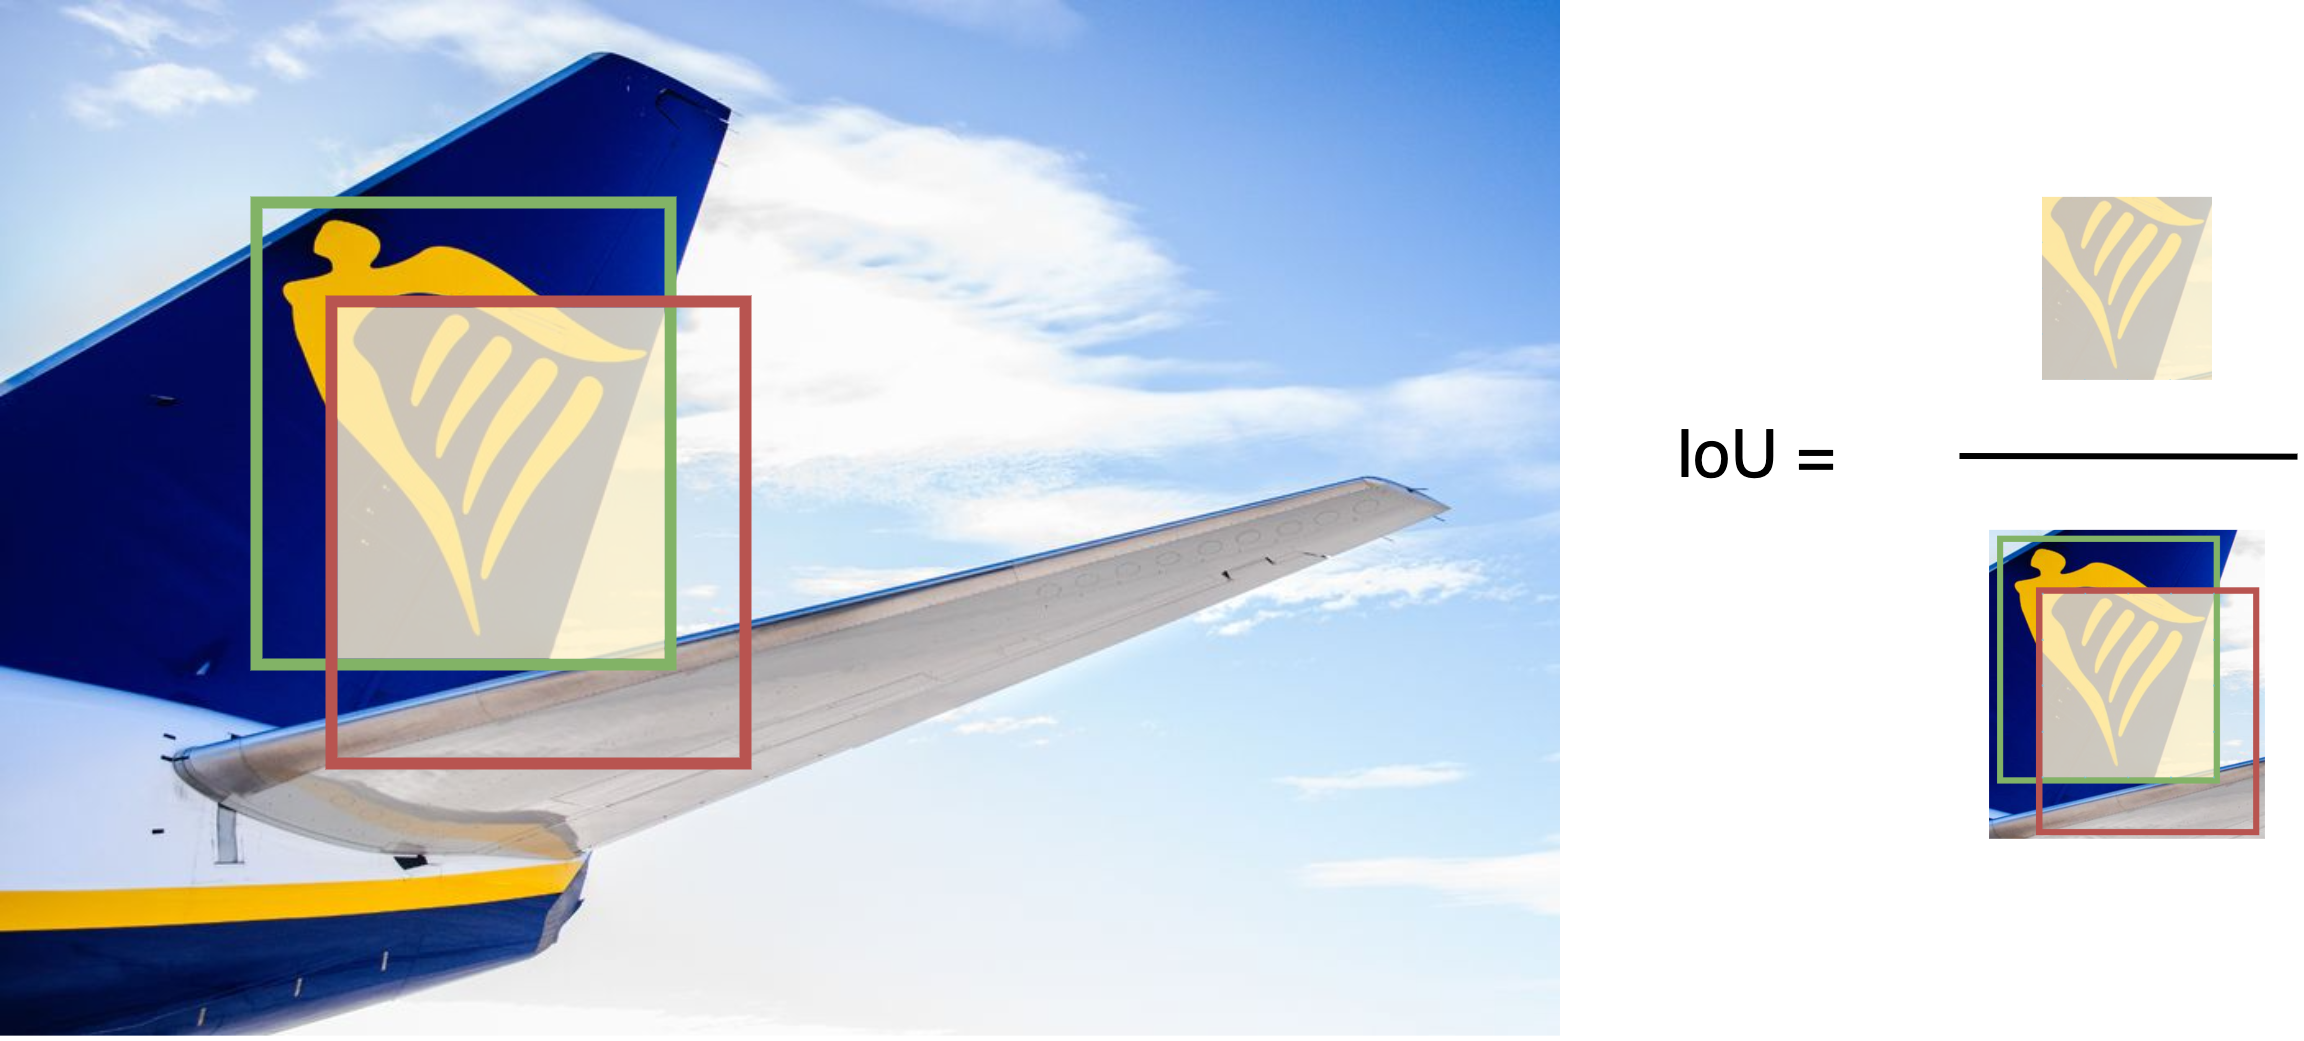
\includegraphics[width=1\textwidth]{images/iou.drawio.png}
	\caption{Intersection over Union (IoU). The green box represents the ground-truth bounding box, the red one represents the predicted bounding box and the intersection is given by the yellow region. Then, the IoU is computed as the ratio of the overlap and union areas.}
	\label{fig:iou}
\end{figure}

\subsubsection{Precision and Recall}
Given the IoU and a threshold $\tau$ it is possible to count the number of:
\begin{itemize}
    \item True Positive (\textbf{TP}): the number of bounding boxes which have a IoU $\geq \tau$ with the ground-truth bounding box.
    \item False Positive (\textbf{FP}): the number of bounding boxes that predict an object which is not actually an object.
    \item False Negative (\textbf{FN}): the number of bounding boxes which have a IoU $< \tau$ with the ground-truth bounding box.
\end{itemize}
Note that the True Negative (TN) are not considered in an object detection task, as this would mean counting as TN the background of the image that contains no object.

Using $TP$, $FP$, $FN$, the Precision $P$ is given by:
\begin{equation} %tp / (tp + fp)
    P = \frac{TP}{TP + FP}
\end{equation}
and the Recall $R$ is given by:
\begin{equation} %tp / (tp + fn)
    R = \frac{TP}{TP + FN}
\end{equation}
Intuitively, precision is the ability of the detector not to recognize a part of the image as an object that is not actually an object, and recall is the ability of the detector to find all objects in the image.
The threshold $\tau$ affects the number of $TP$, $FP$, $FN$ and thus the value of precision and recall.
For this reason, given a value for $\tau$ (e.g. $\tau = 0.5$), computing the precision or recall at $\tau = 0.5$ is denoted by $P@.5$ and $R@.5$ respectively.

\subsubsection{Mean Average Precision}
Average Precision (AP) is calculated as the weighted average of precisions at each threshold; the weight is the increase in recall from the prior threshold. For values of $\tau \in T$, where $T = [0.50, 0.55, 0.60,\, ..., \, 0.95 ]$, the AP computed using the thresholds in $T$ and denoted by AP@.5:.95 is given by:
\begin{equation}
    AP = \sum_{i=1}^{|T| - 1}(R@\tau_i - R@\tau_{i+1} ) * P@\tau_{i}
\end{equation}
Finally, given $k$ different classes, the mAP is the average of the APs among each class:
\begin{equation}
    mAP = \frac{1}{k} \sum_{i=1}^{k} AP_i
\end{equation}

\subsection{100 Classes}

As described in \autoref{chap:methods}, the class-agnostic logo detector represents the first stage of the system and works in combination with the CIL model to achieve incremental learning logo detection and recognition.

\subsubsection{Training using the 30 classes of the initial task}
As with the CIL classifier, the first experiments with the logo detector focus on the top-100 classes of the dataset (where top-100 refers to the 100 classes with the highest number of samples, see \autoref{sec:cil-top100}).
Given the nature of the problem, in a real scenario, the detector is trained using only those classes available for the CIL model at task 0.
In the CIL setup described in \autoref{sec:exp-setup}, the initial task consists of 30 classes.

For this reason, in the top-100 classes setup, the detector is trained for 30 epochs with the SGD optimizer using only those 30 classes available at task 0.
Note that, as described before, the 30 classes correspond to those considered by the CIL model at task 0.

During the training of the detector, the object loss, box loss (see \autoref{sec:yolo} and \autoref{eq:yolo-loss}) and the mAP@.5 are monitored on the validation set.
The performance shown in \autoref{fig:exp-det_100} considers only the 30 classes used for training, which is useful for analyzing the training phase, but given the incremental learning setup, we expect the class-agnostic logo detector to perform well on all the 100 classes.
For this purpose, the detector is evaluated considering the mAP@.5 on the test set combining the initial 30 classes and the remaining 70.
This evaluation represents a real-world scenario and is therefore the most reliable and most suitable for evaluating the detector.
The results of the evaluation are shown in \autoref{table:exp-det_100}.


\subsubsection{Generalization capabilities of the class-agnostic logo detector}
To better study the generalization capabilities of the detector trained on 30 classes to the remaining 70, the detector is compared with a new one trained on all the 100 classes.
This detector can be considered as a baseline with respect to the generalization capabilities of the detector trained on 30 classes: the smaller the gap between the performance of these two models, the better the generalization capabilities.
This new detector is trained for 30 epochs using the 100 classes and, as before, object loss, box loss and mAP@.5 are monitored on the validation set. The comparison between the two detectors is shown in \autoref{fig:exp-det_100}.

As we can see from \autoref{fig:exp-det_100}, the performance of detectors trained on 100 and 30 classes is quite similar.
However, a crucial aspect of this training results, is that these metrics consider all and only those classes on which the model is trained, thus 30 classes and 100 classes.
The fact that the detectors achieve the same performance is a sign that they accomplish similar results in detecting logos across a different number of classes.
However, the real comparison consists in considering the mAP@0.5 for each detector, computed on the test set of all the 100 classes. This comparison is shown in \autoref{table:exp-det_100}. As we can see, the detector trained on 30 classes does not generalize well on the remaining 70.
In fact, comparing the mAP@.5 computed on the test set composed of all 100 classes, with the mAP@.5 obtained on the validation at the last training epochs (shown in \autoref{fig:exp-det_100}), the performance drops from about 0.97 to 0.75.

In contrast, the detector trained on all the 100 classes, obtains a mAP@.5 on the test set of 0.982, which is consistent with the performance obtained on the validation set at the last training epochs.
However, it must be considered that, since this detector is trained using 70 more classes, it has more training samples at its disposal, hence more data from which to acquire knowledge of a logo.


\begin{table}[H]
    \centering
    \begin{tabular}{c|c|c|c|c}
        \hline
        \textbf{Model} &
        \textbf{Precision} &
        \textbf{Recall} &
        \textbf{mAP@.5} &
        \textbf{mAP@.5:.95} \\
        \hline
        \hline
DET\_class-agnostic\_30cls&0.784&0.659&0.75&0.542\\
DET\_class-agnostic\_100cls&0.944&0.972&0.982&0.776\\
\hline
\end{tabular}
\caption{Precision, Recall, mAP@.5 and mAP@.5:.95 obtained by the detector trained on 30 classes (DET\_class-agnostic\_30cls) and the one trained on 100 classes (DET\_class-agnostic\_10cls). The performance refers to the test set composed of all the 100 classes.}
    \label{table:exp-det_100}
\end{table}
%\newpage

\begin{figure}[H]
	\centering
	\subfloat[\centering mAP@.5]{{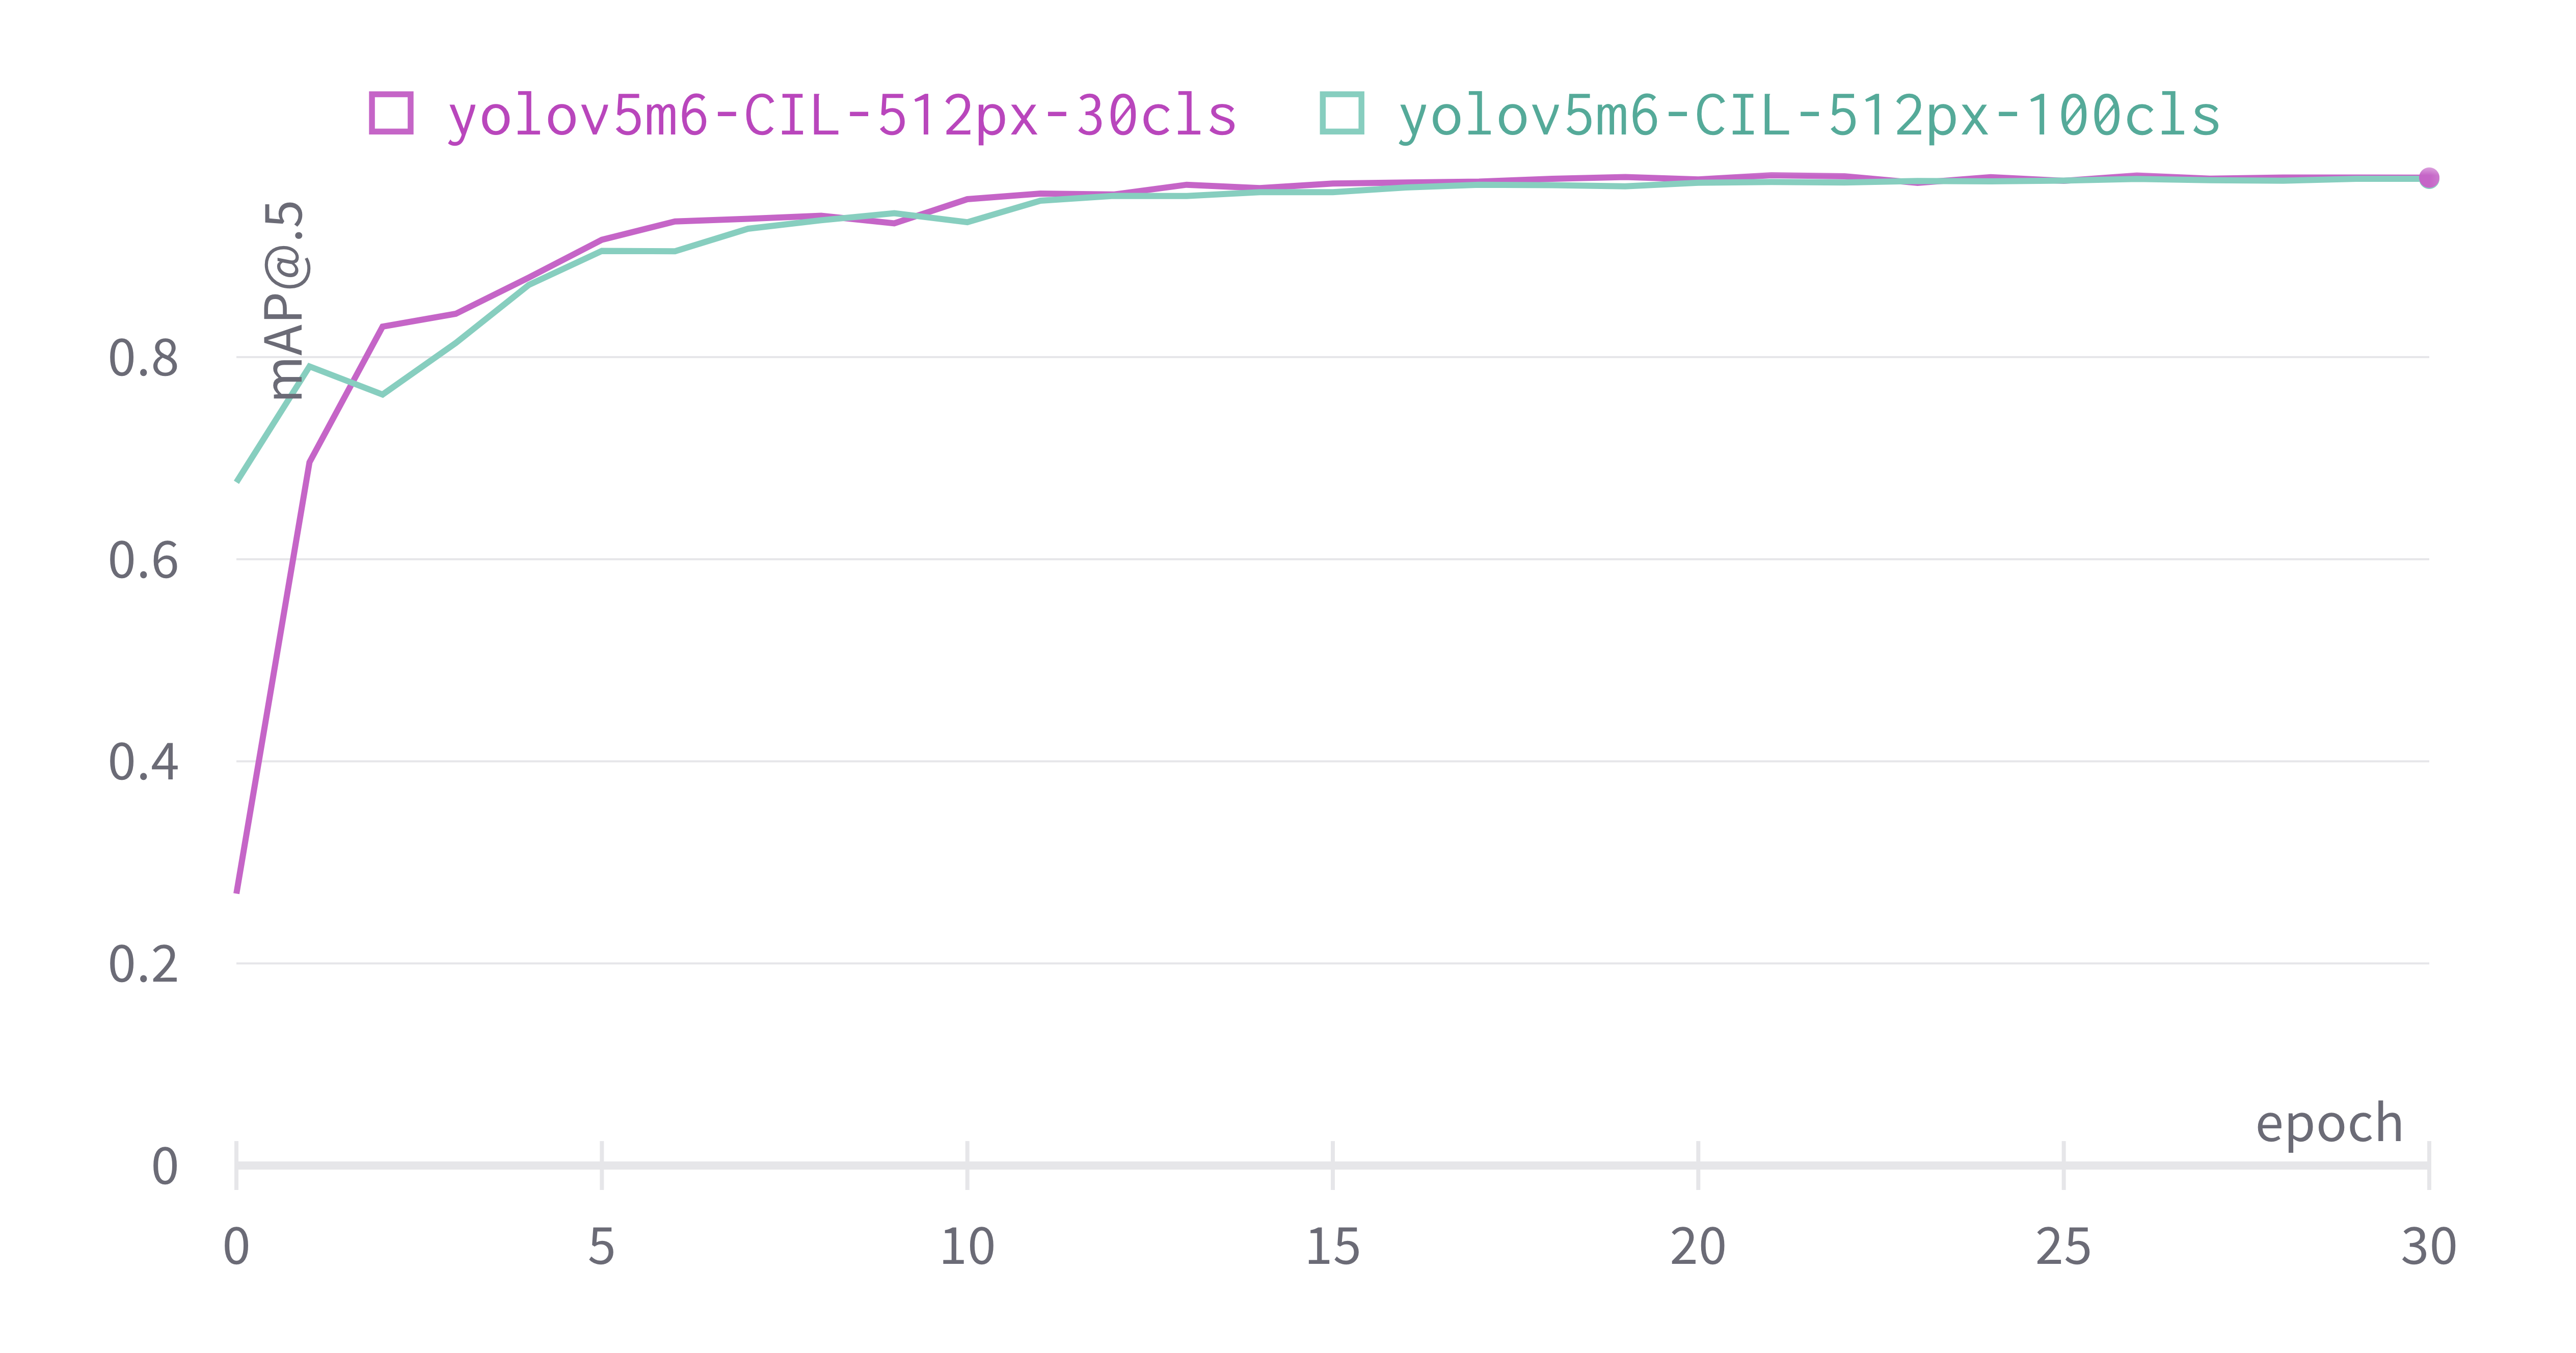
\includegraphics[width=0.50\textwidth]{images/exp/exp-det-map.png} }}%
    %\qquad
	\subfloat[\centering Box loss]{{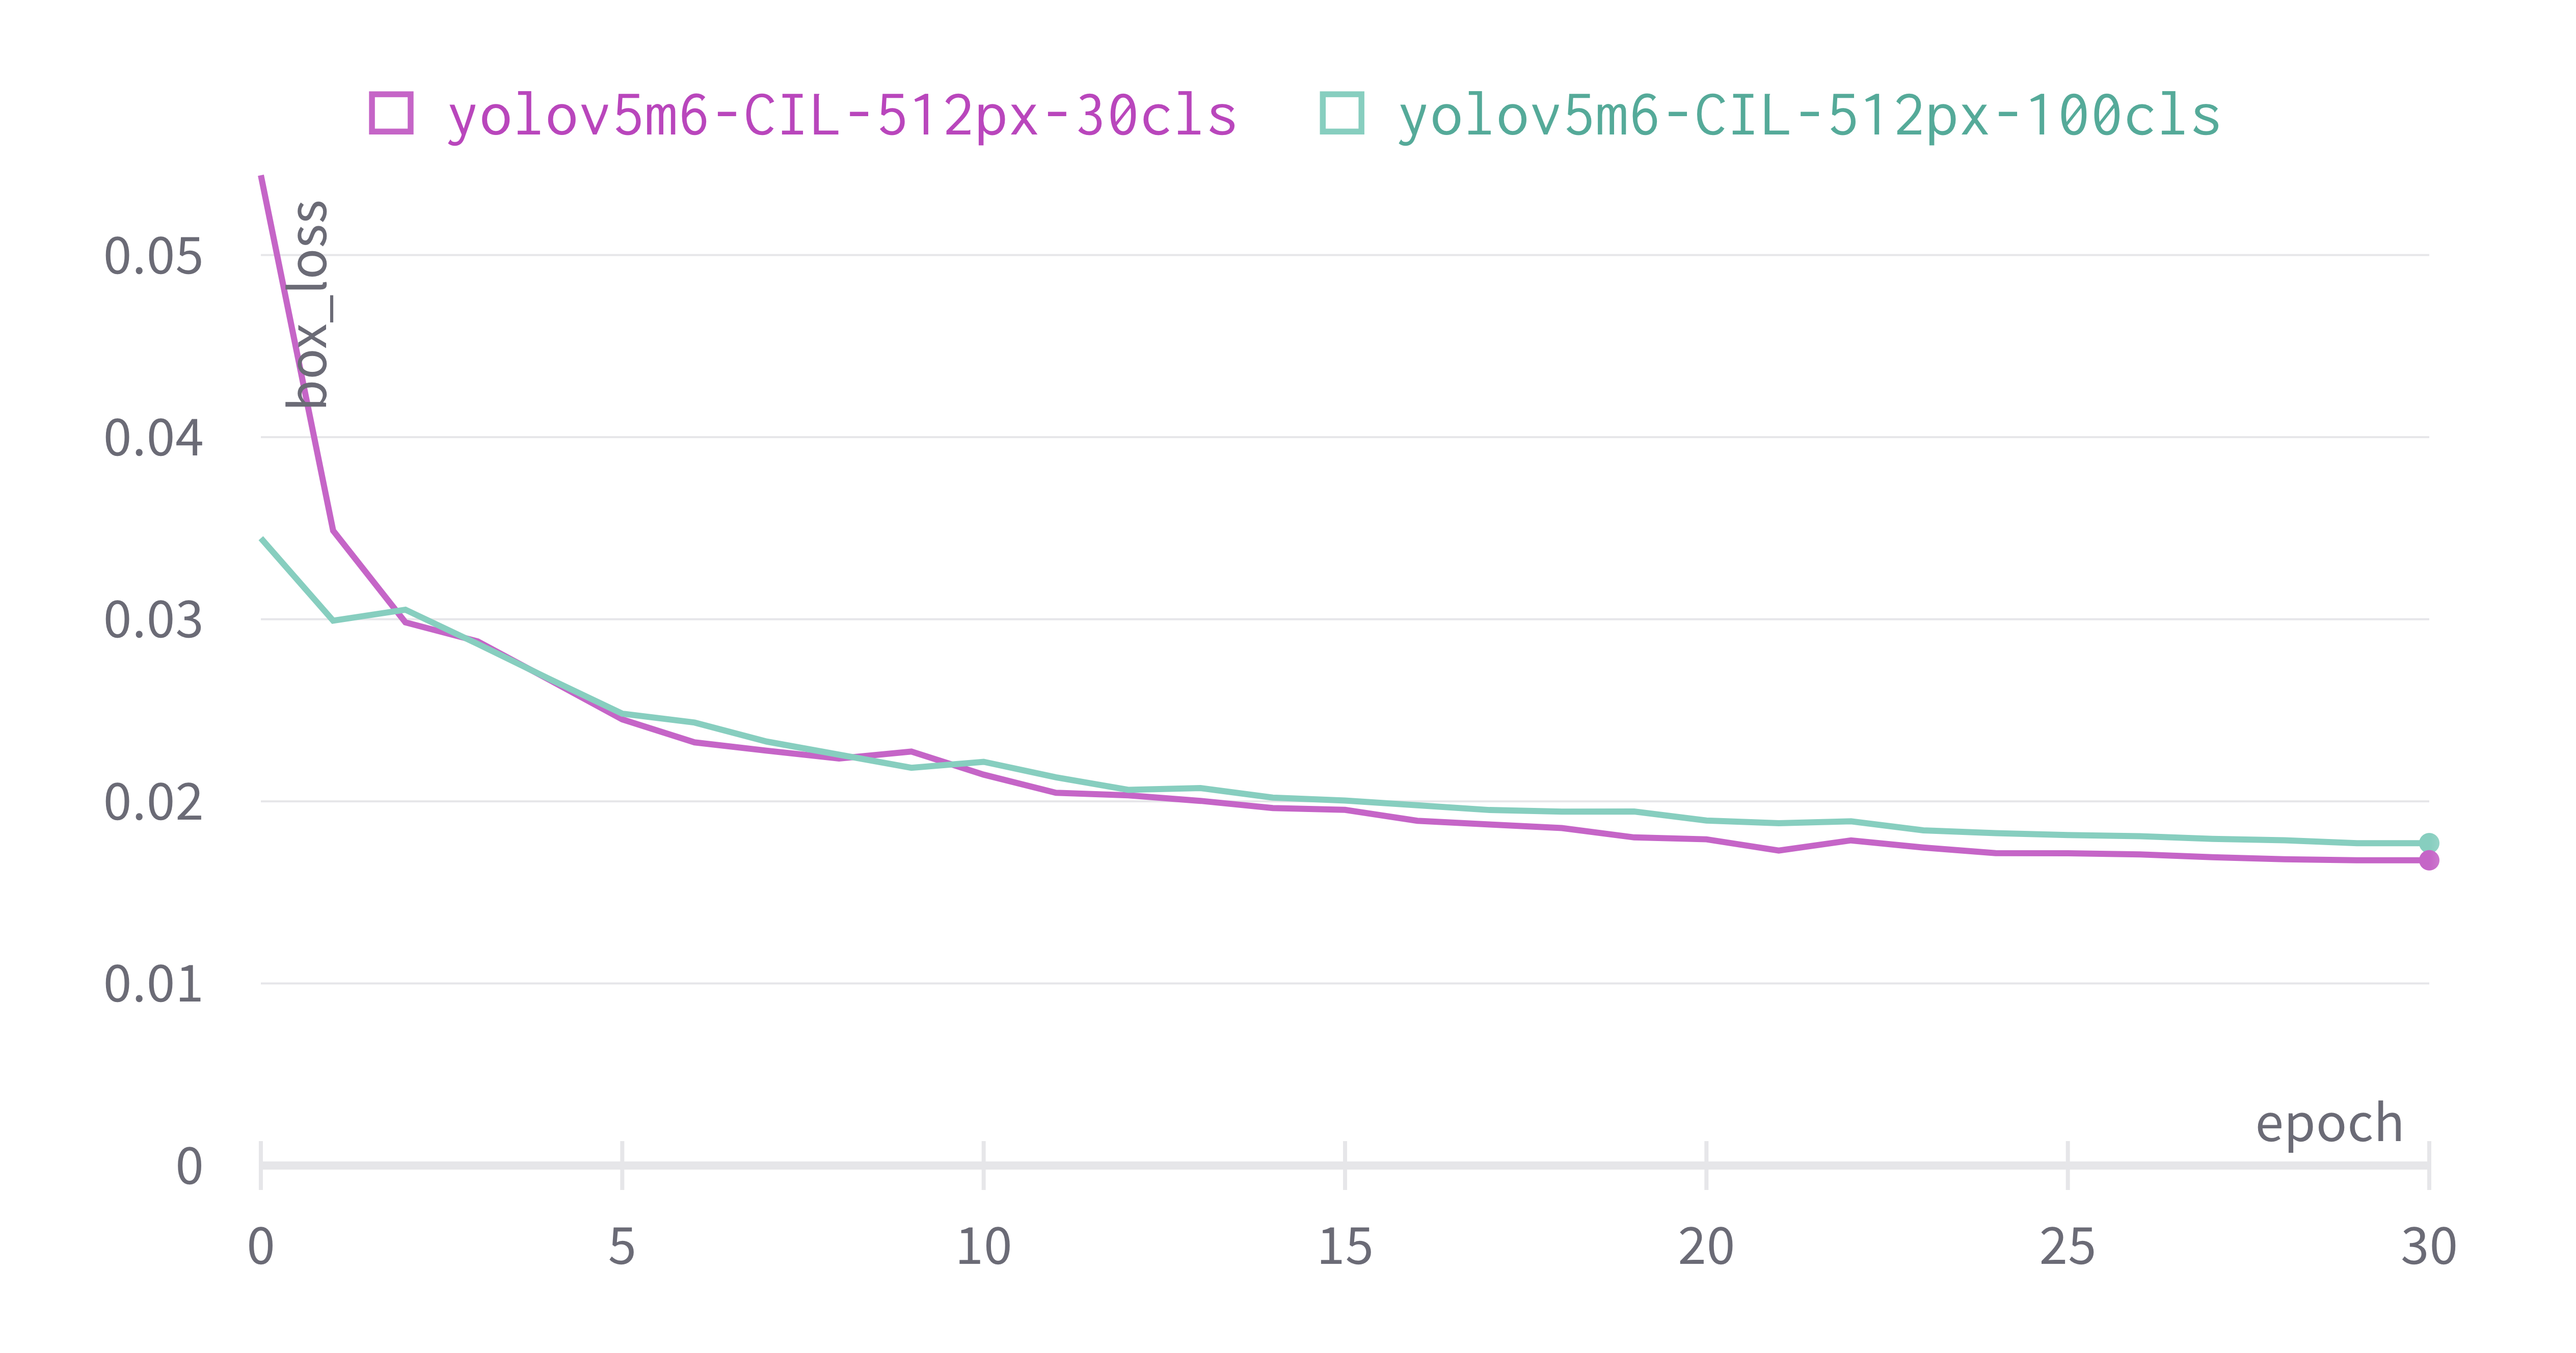
\includegraphics[width=0.50\textwidth]{images/exp/exp-det-box_loss.png} }}%
    \qquad
	\subfloat[\centering Object loss]{{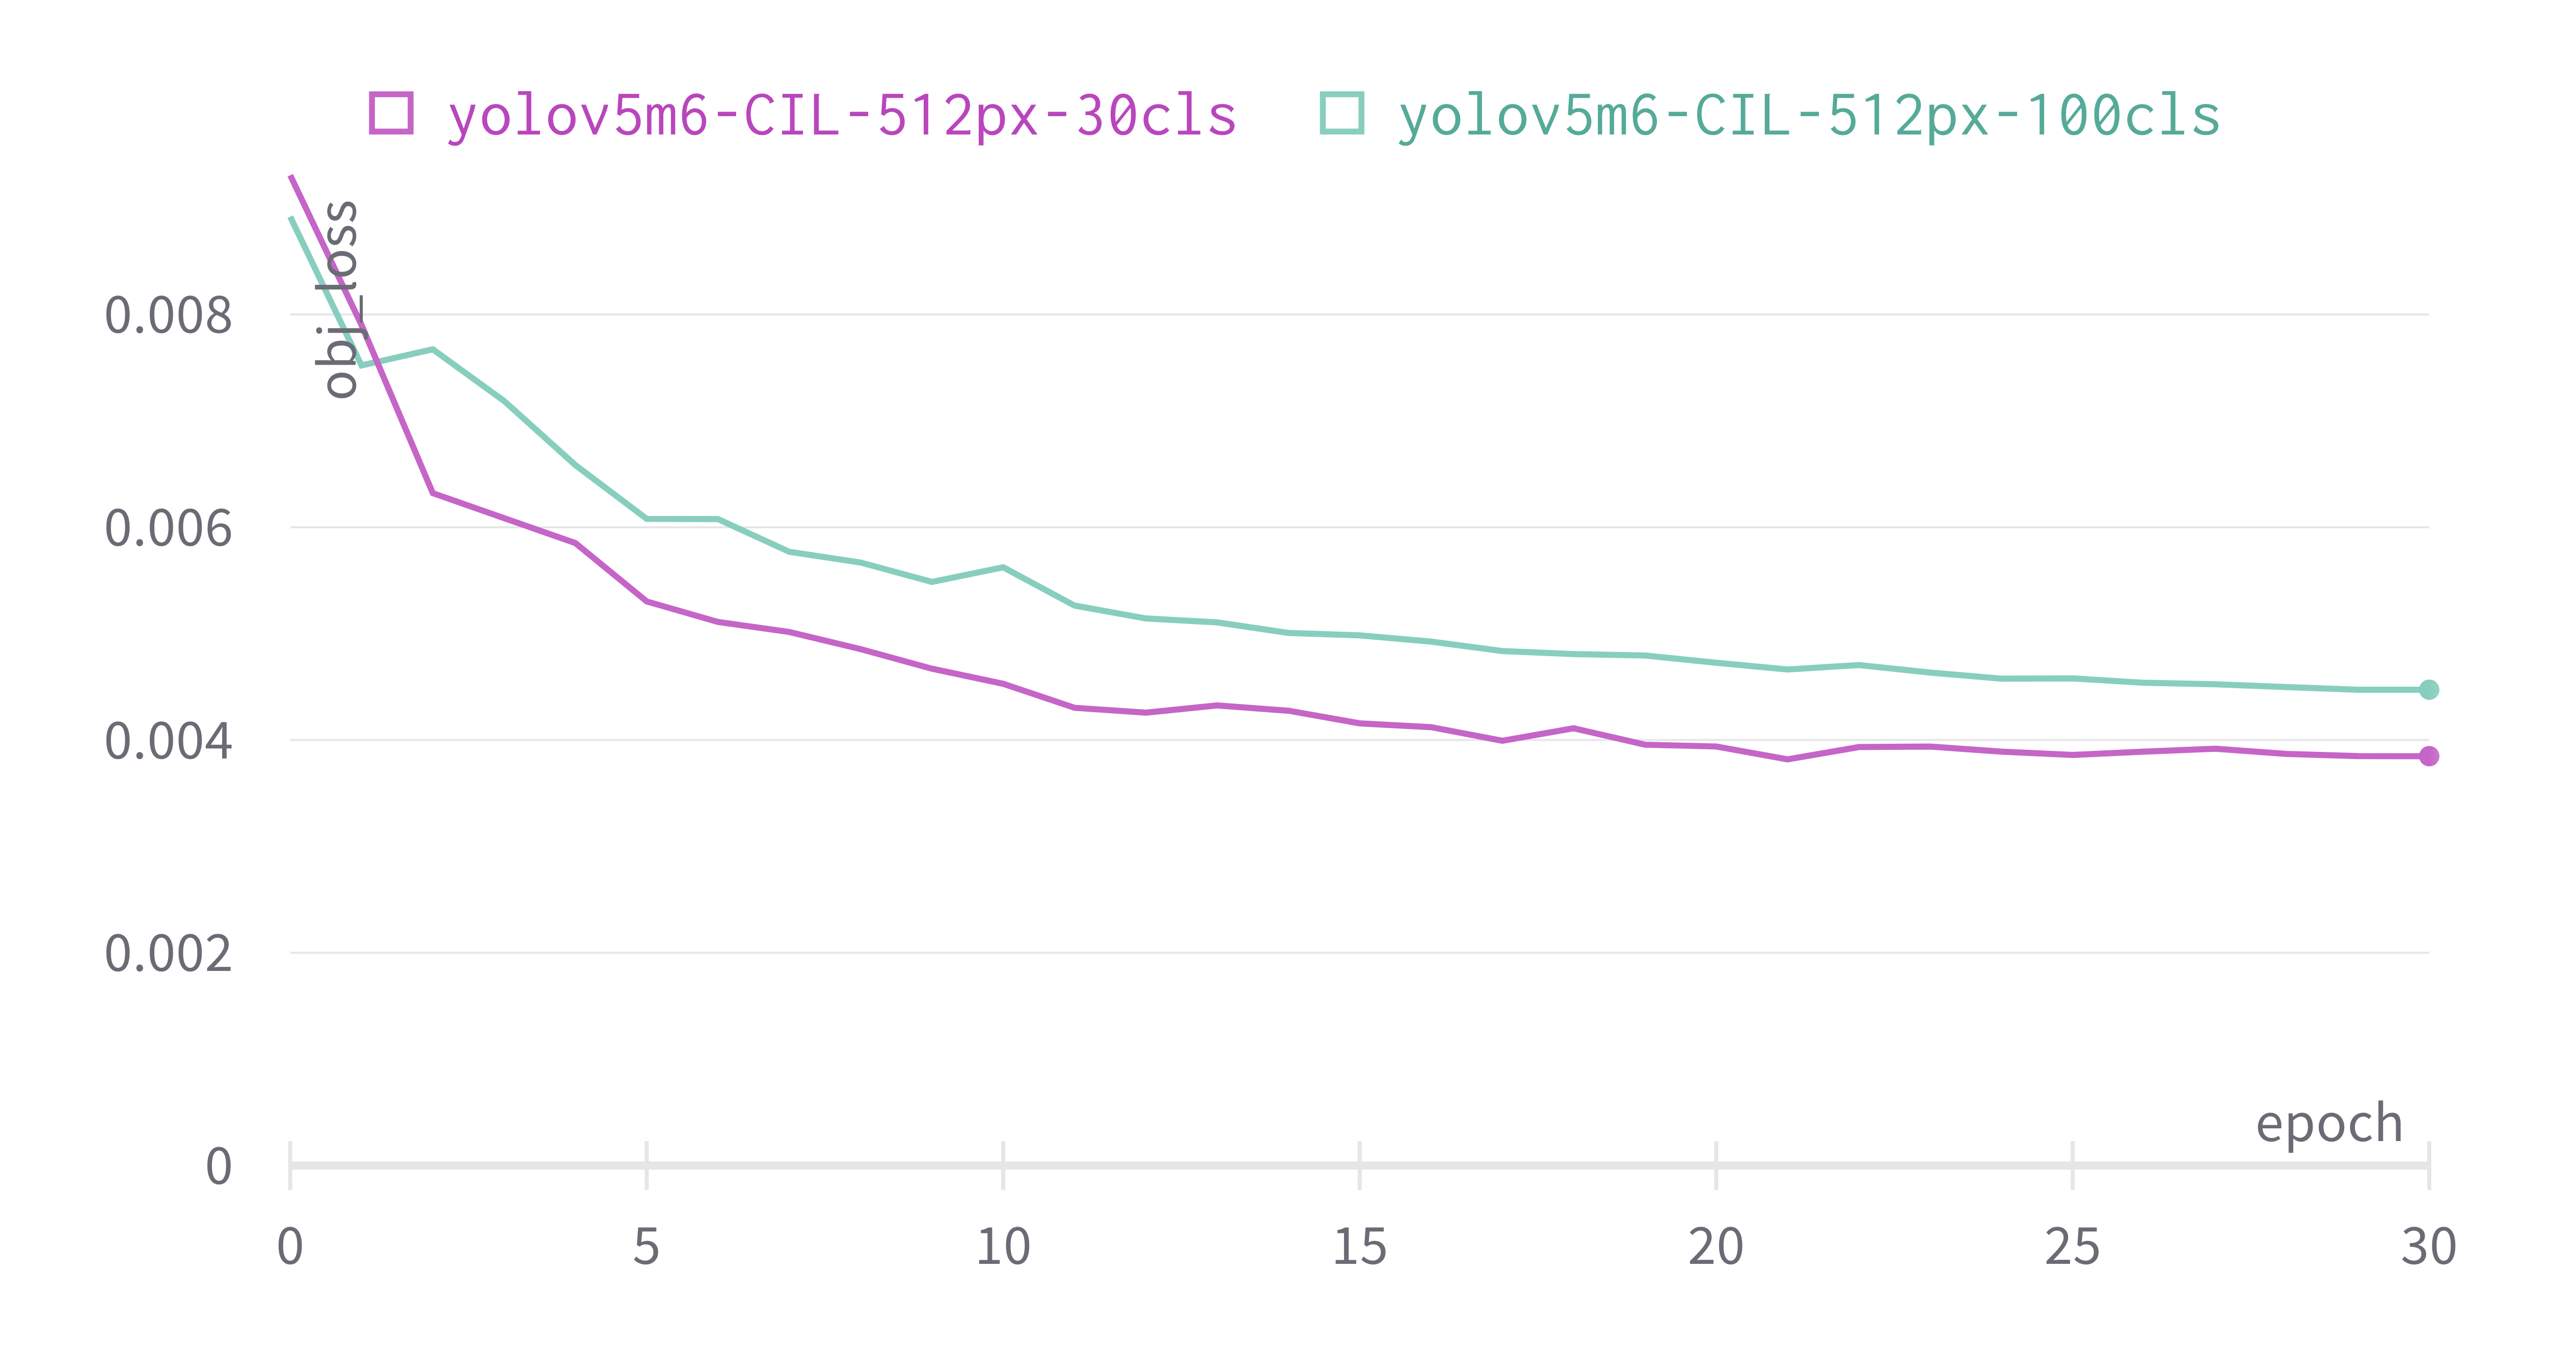
\includegraphics[width=0.50\textwidth]{images/exp/exp-det-obj_loss.png} }}%
    \caption{Performance comparison between the class-agnostic logo detector trained on 30 classes and the one trained on 100 classes. The plots show the mAP@.5, box loss and object loss on the validation set at each training epoch. Note that these performance are computed on the validation set of each model, thus using 30 and 100 classes respectively.}%
	\label{fig:exp-det_100}
\end{figure}


\subsection{2993 Classes}
\label{sec:2993-detector}
The experiments conducted in the previous section are repeated considering the 2993-class setup (see \autoref{sec:exp-setup}), which consists of 1000 classes used at the initial task and 250 classes added at each incremental learning task.
This section evaluates the detector's ability to scale from 100 classes to 2993 classes.

As in the case of the setup of the top-100 classes, the detector is trained for 30 epochs using the SGD optimizers on the first 1000 classes of the initial task. Then the evaluation metrics are computed on the test set of these 1000 classes combined with the remaining 1993 classes, thus on the entire dataset consisting of 2993 classes in total.

During the training, object loss, box loss (see \autoref{sec:yolo} and \autoref{eq:yolo-loss}) and mAP@.5 are monitored on the validation set consisting of the 1000 classes used for training.
As we can see in \autoref{fig:exp-det_2993}, the mAP@.5 of the model computed on the validation set is lower than the 30-class or 100-class setup.
This is because recognizing 1000 different logos is a more difficult task than recognizing 30 or 100 different logos.

Apart from the performance on the validation set obtained during training, the most useful insights are obtained by evaluating the detector on the test set consisting of all 2993 classes. The results are shown in \autoref{table:exp-det_2993}. As we can seen, the mAP@.5 is very similar to the 30-class setup (0.706 vs 0.75).

Another important comparison is between the detector trained on 1000 classes and that trained on all 2993 classes, as done for the 100-class setup.
This is done to assess the generalization capabilities of the detector trained on 1000 classes when tested on all classes.
The results of training of the detector trained on all 2993 classes are shown in \autoref{fig:exp-det_2993} and the final performance obtained by testing it on the entire dataset is shown in \autoref{table:exp-det_2993}.

From the results shown in \autoref{table:exp-det_100} we can see that the gap in mAP@.5 between the detector trained on 30 classes and the one trained on 100 classes is quite large. However, from the results obtained in \autoref{table:exp-det_2993} emerges that, in contrast to the previous setup, this gap in mAP@.5 is reduced: \todo{Queste performance sono relative all'epoca 16 di training. Appena ho accesso al server aggiorno la performance ottenuta all'epoca 30}0.706 in the 1000-class setup vs. 0.73 in the 2993-class setup.
This observation reveals that even if the detector is only trained on 1000 classes, it generalize well, i.e. is able to effectively detect, the remaining 1993 classes.

This is a fundamental result for the entire system, as it is evidence in support of the claim made in \autoref{chap:introduction}, where it is assumed that it is not necessary to also develop an incremental learning detector, since the idea of what a generic logo is can be learned and well approximated using only an initial set of logos. The subsequent creation of new logos will not disrupt the general idea of a logo.

\begin{table}[H]
    \centering
    \begin{tabular}{c|c|c|c|c}
        \hline
        \textbf{Model} &
        \textbf{Precision} &
        \textbf{Recall} &
        \textbf{mAP@.5} &
        \textbf{mAP@.5:.95} \\
        \hline
        \hline
DET\_class-agnostic\_1000cls&0.704&0.666&0.706&0.465\\
DET\_class-agnostic\_2993cls&0.704&0.781&0.73&0.495\\
\hline
\end{tabular}
\caption{Precision, Recall, mAP@.5 and mAP@.5:.95 obtained by the detector trained on 1000 classes (DET\_class-agnostic\_1000cls) and that trained on 2993 classes (DET\_class-agnostic\_2993cls). The performance refers to the test set composed of all the 2993 classes.}
    \label{table:exp-det_2993}
\end{table}
%\newpage

\begin{figure}[H]
	\centering
	\subfloat[\centering mAP@.5]{{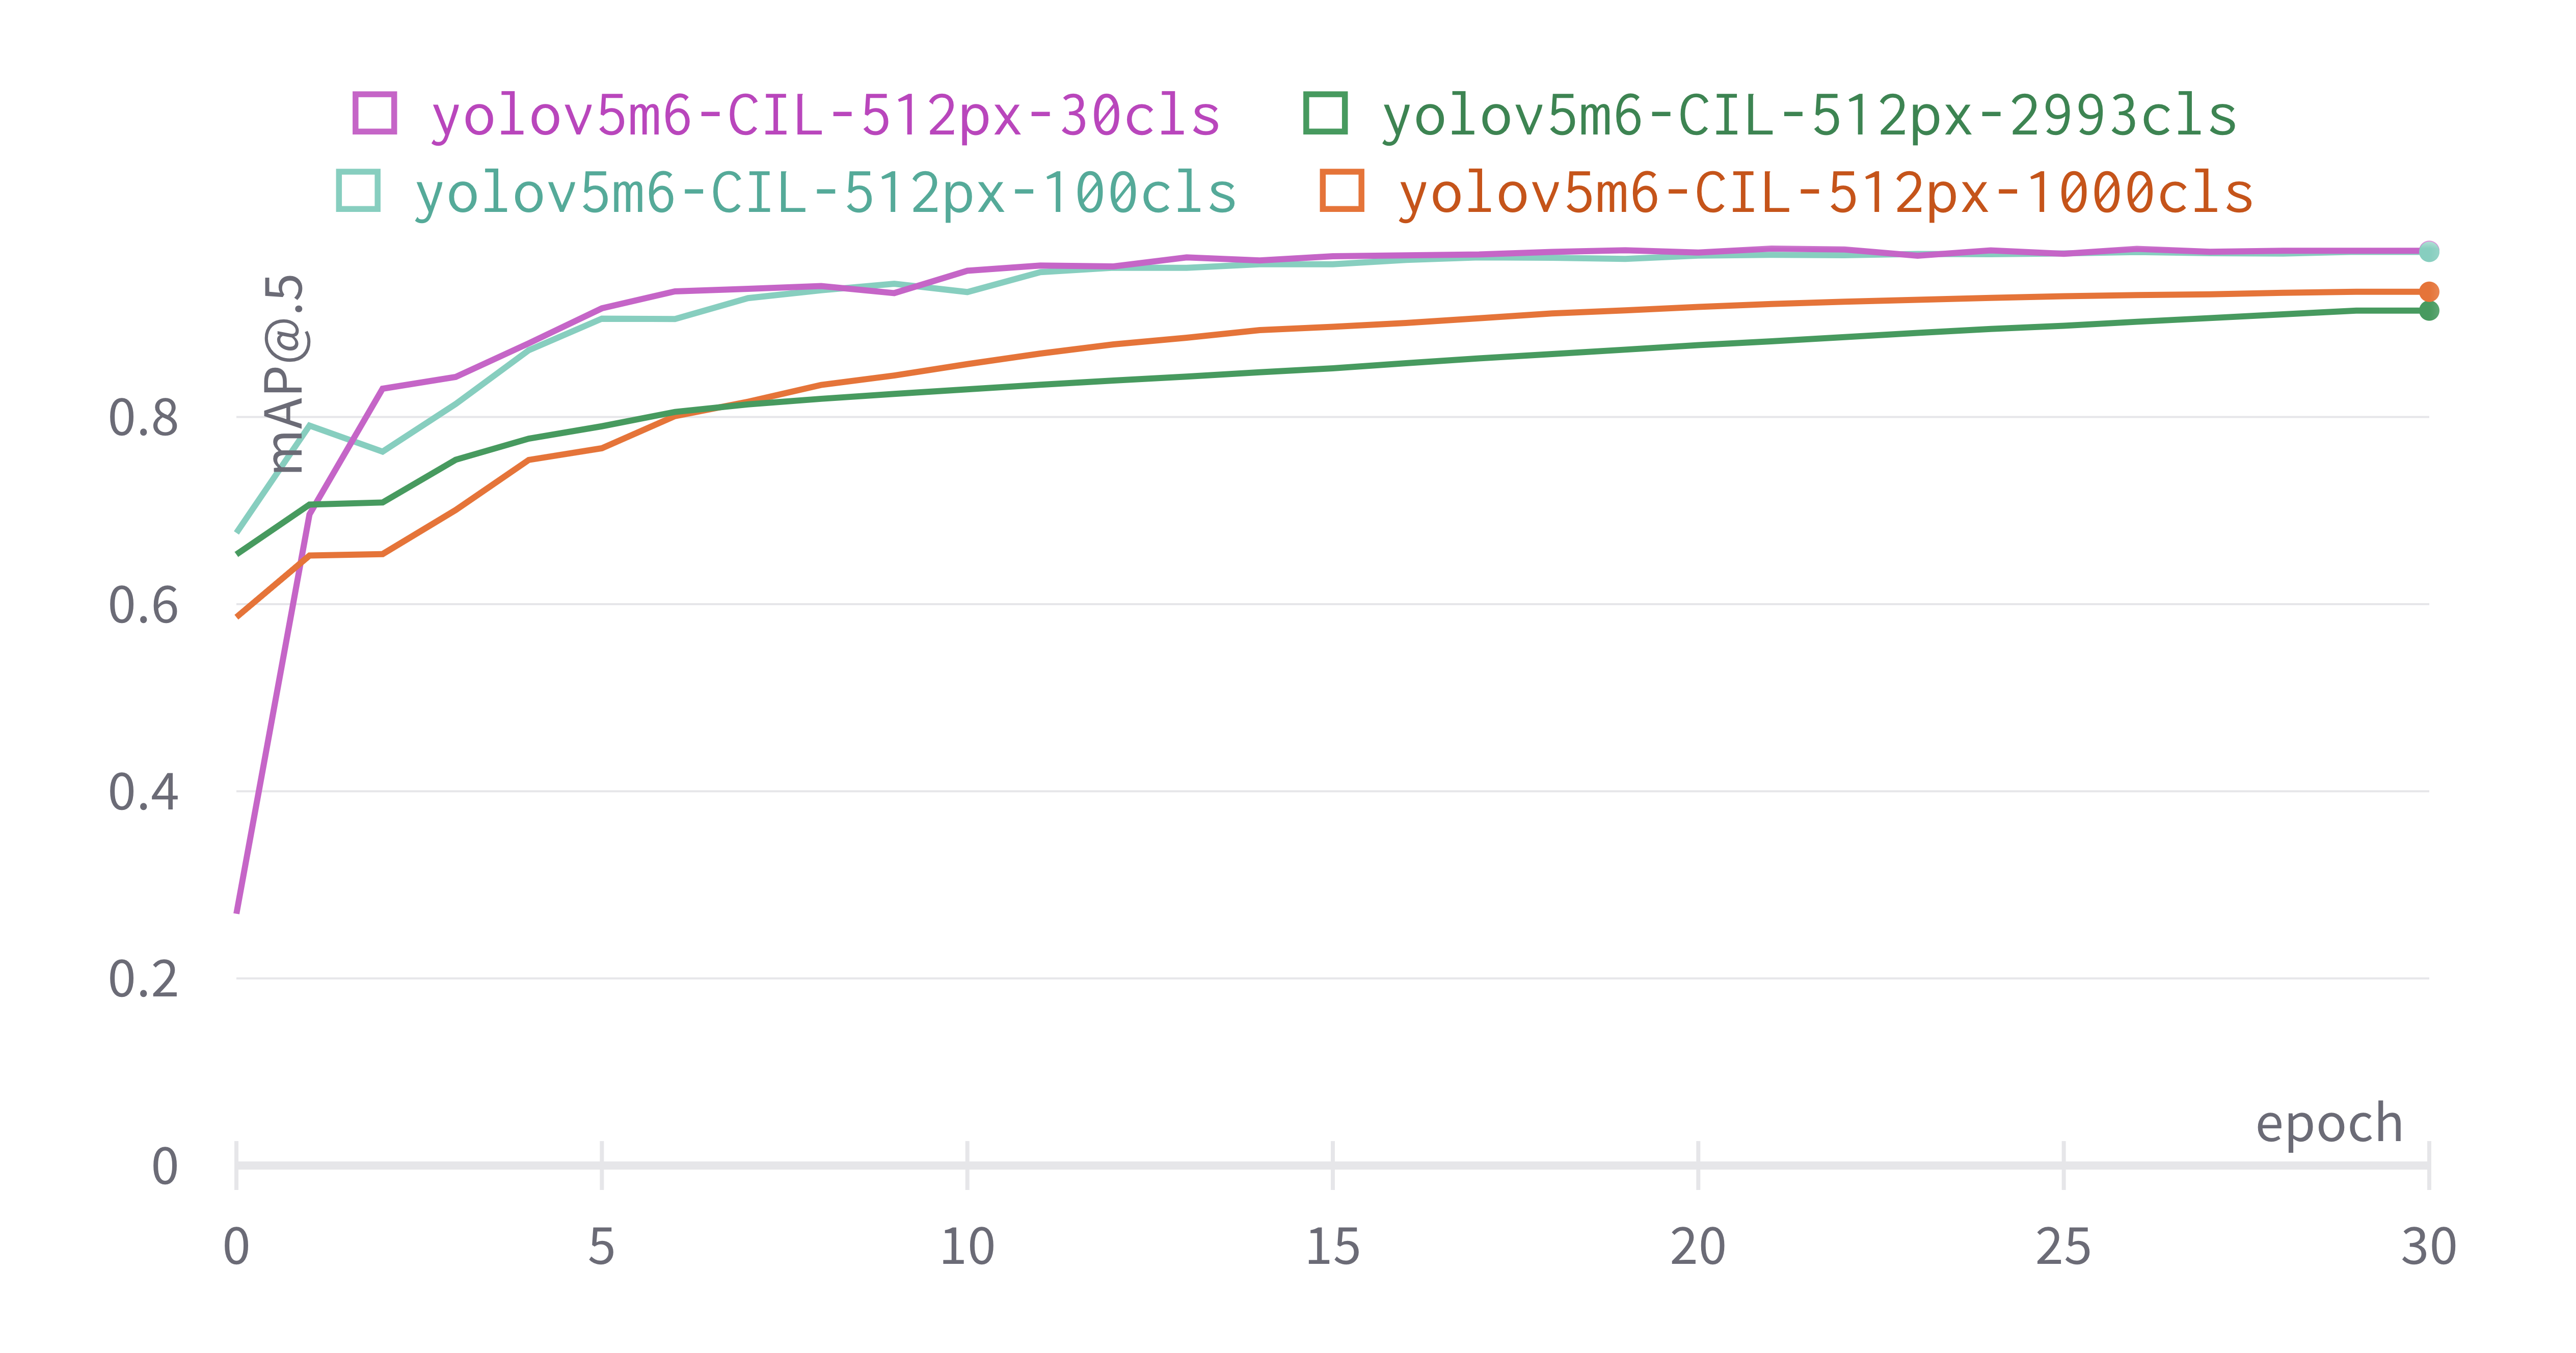
\includegraphics[width=0.50\textwidth]{images/exp/exp-det-map-2993.png} }}%
    %\qquad
	\subfloat[\centering Box loss]{{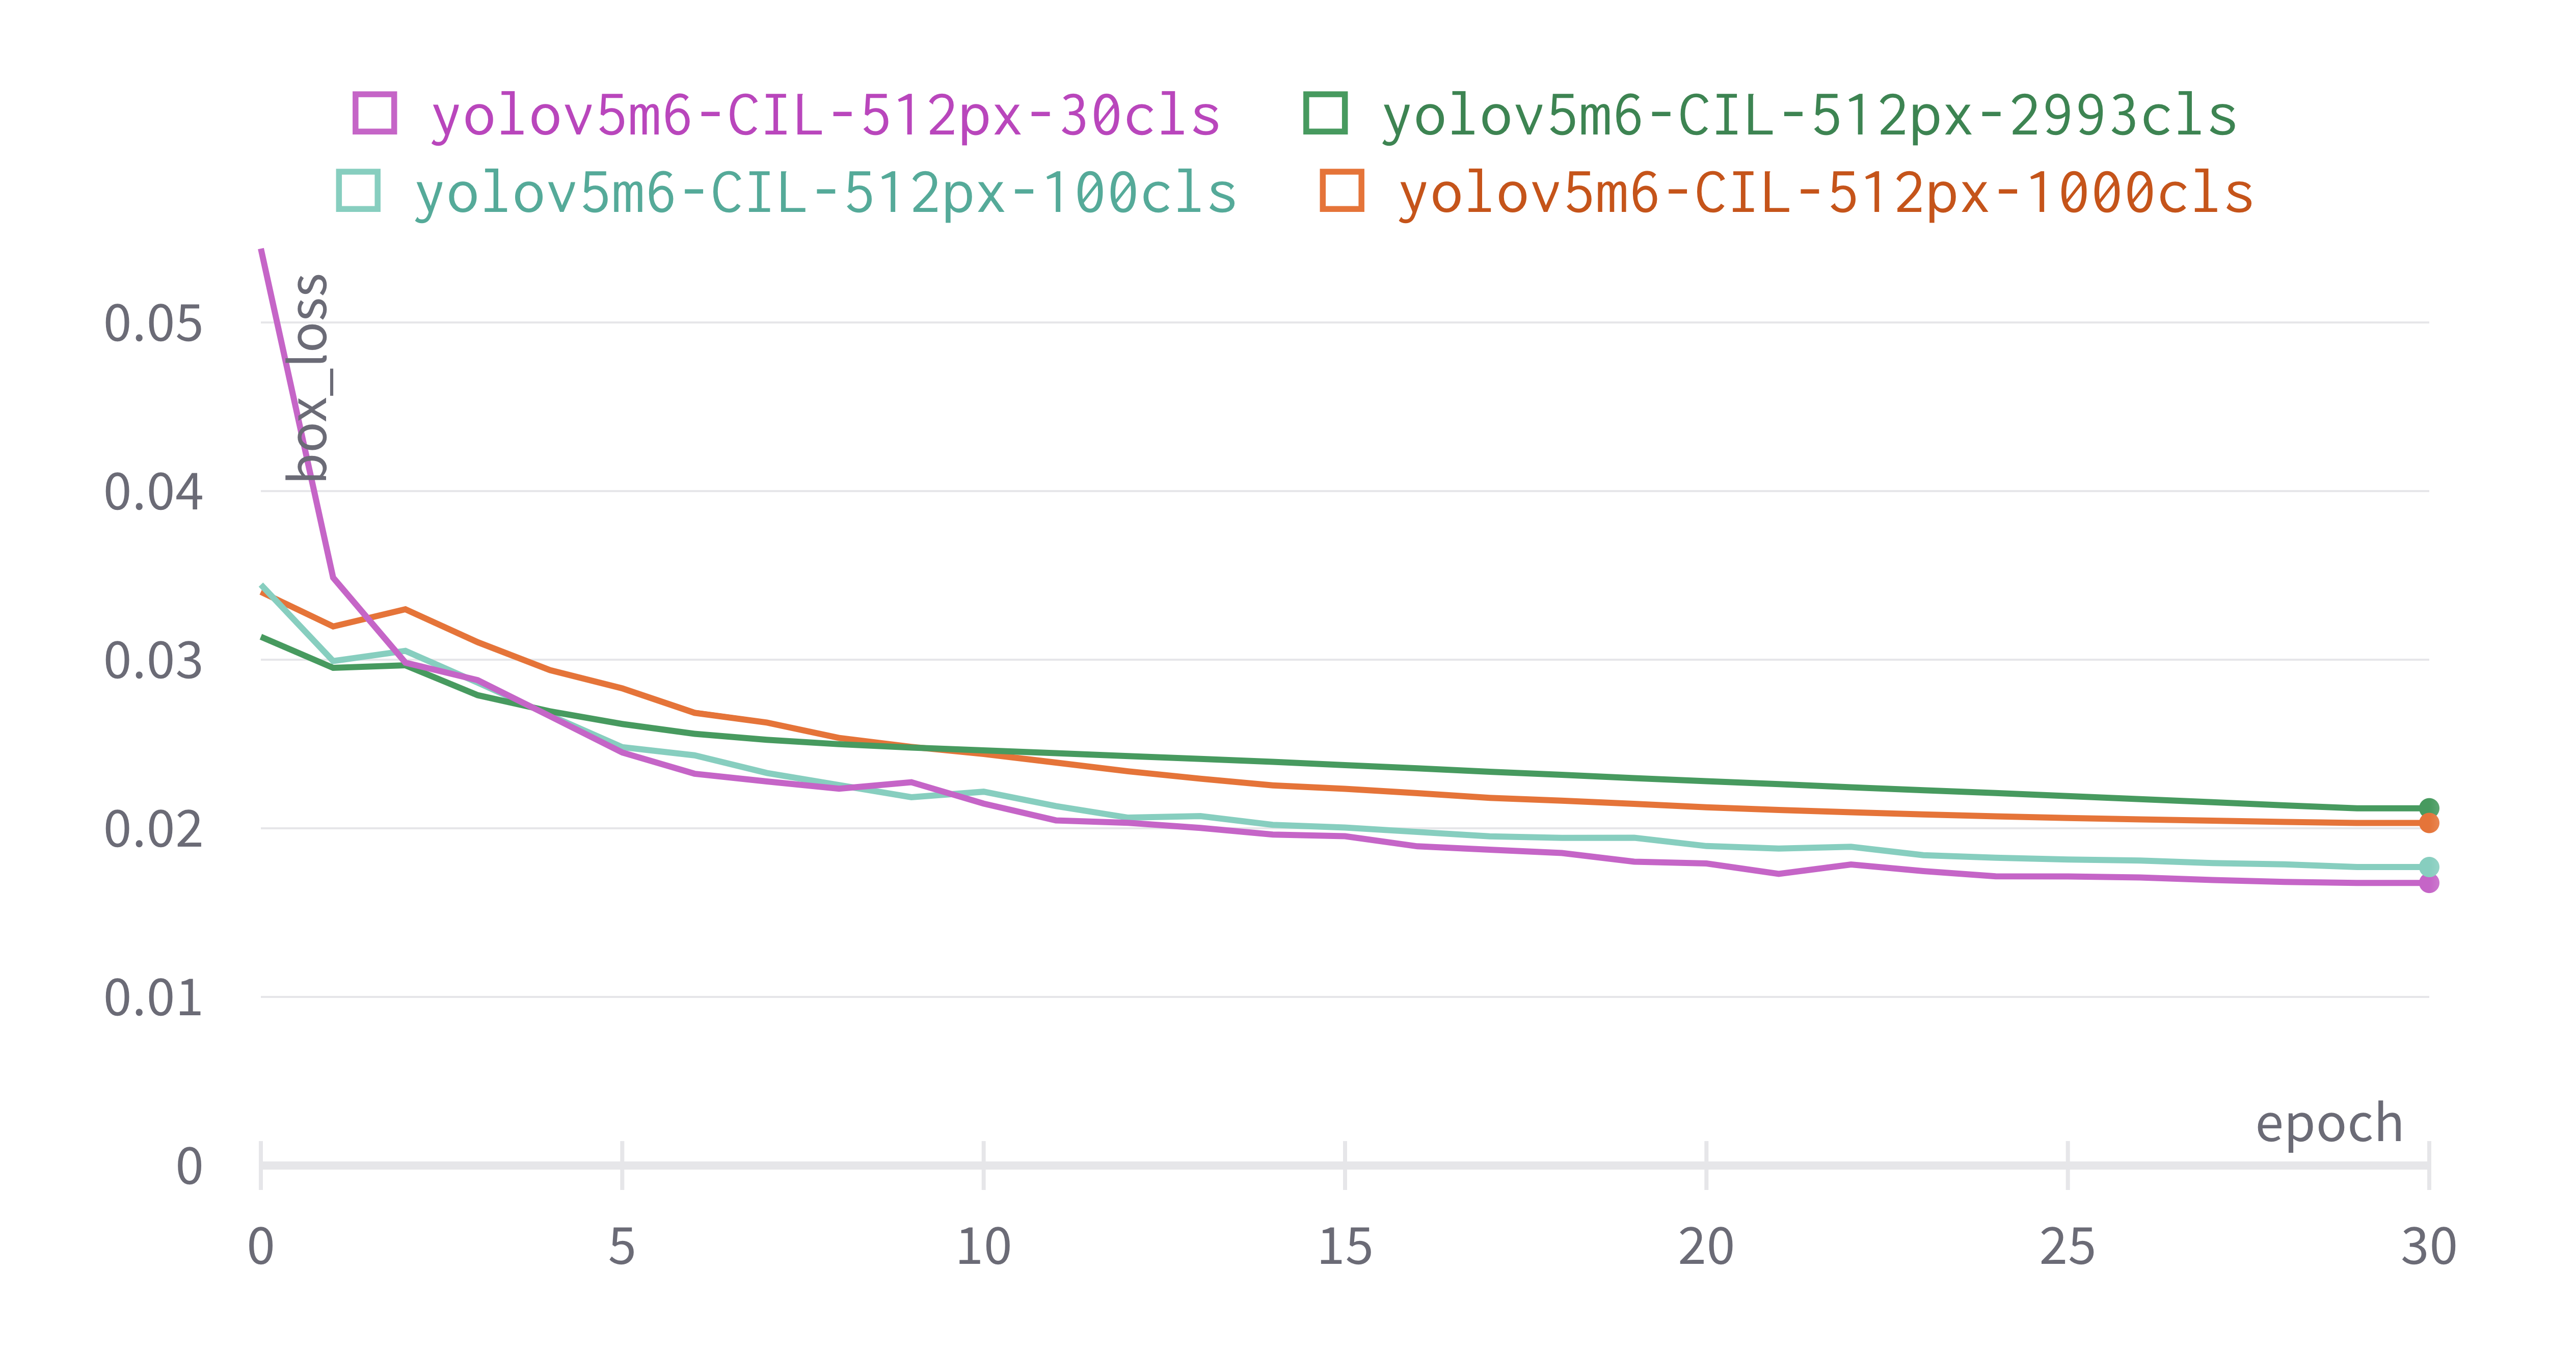
\includegraphics[width=0.50\textwidth]{images/exp/exp-det-box_loss-2993.png} }}%
    \qquad
	\subfloat[\centering Object loss]{{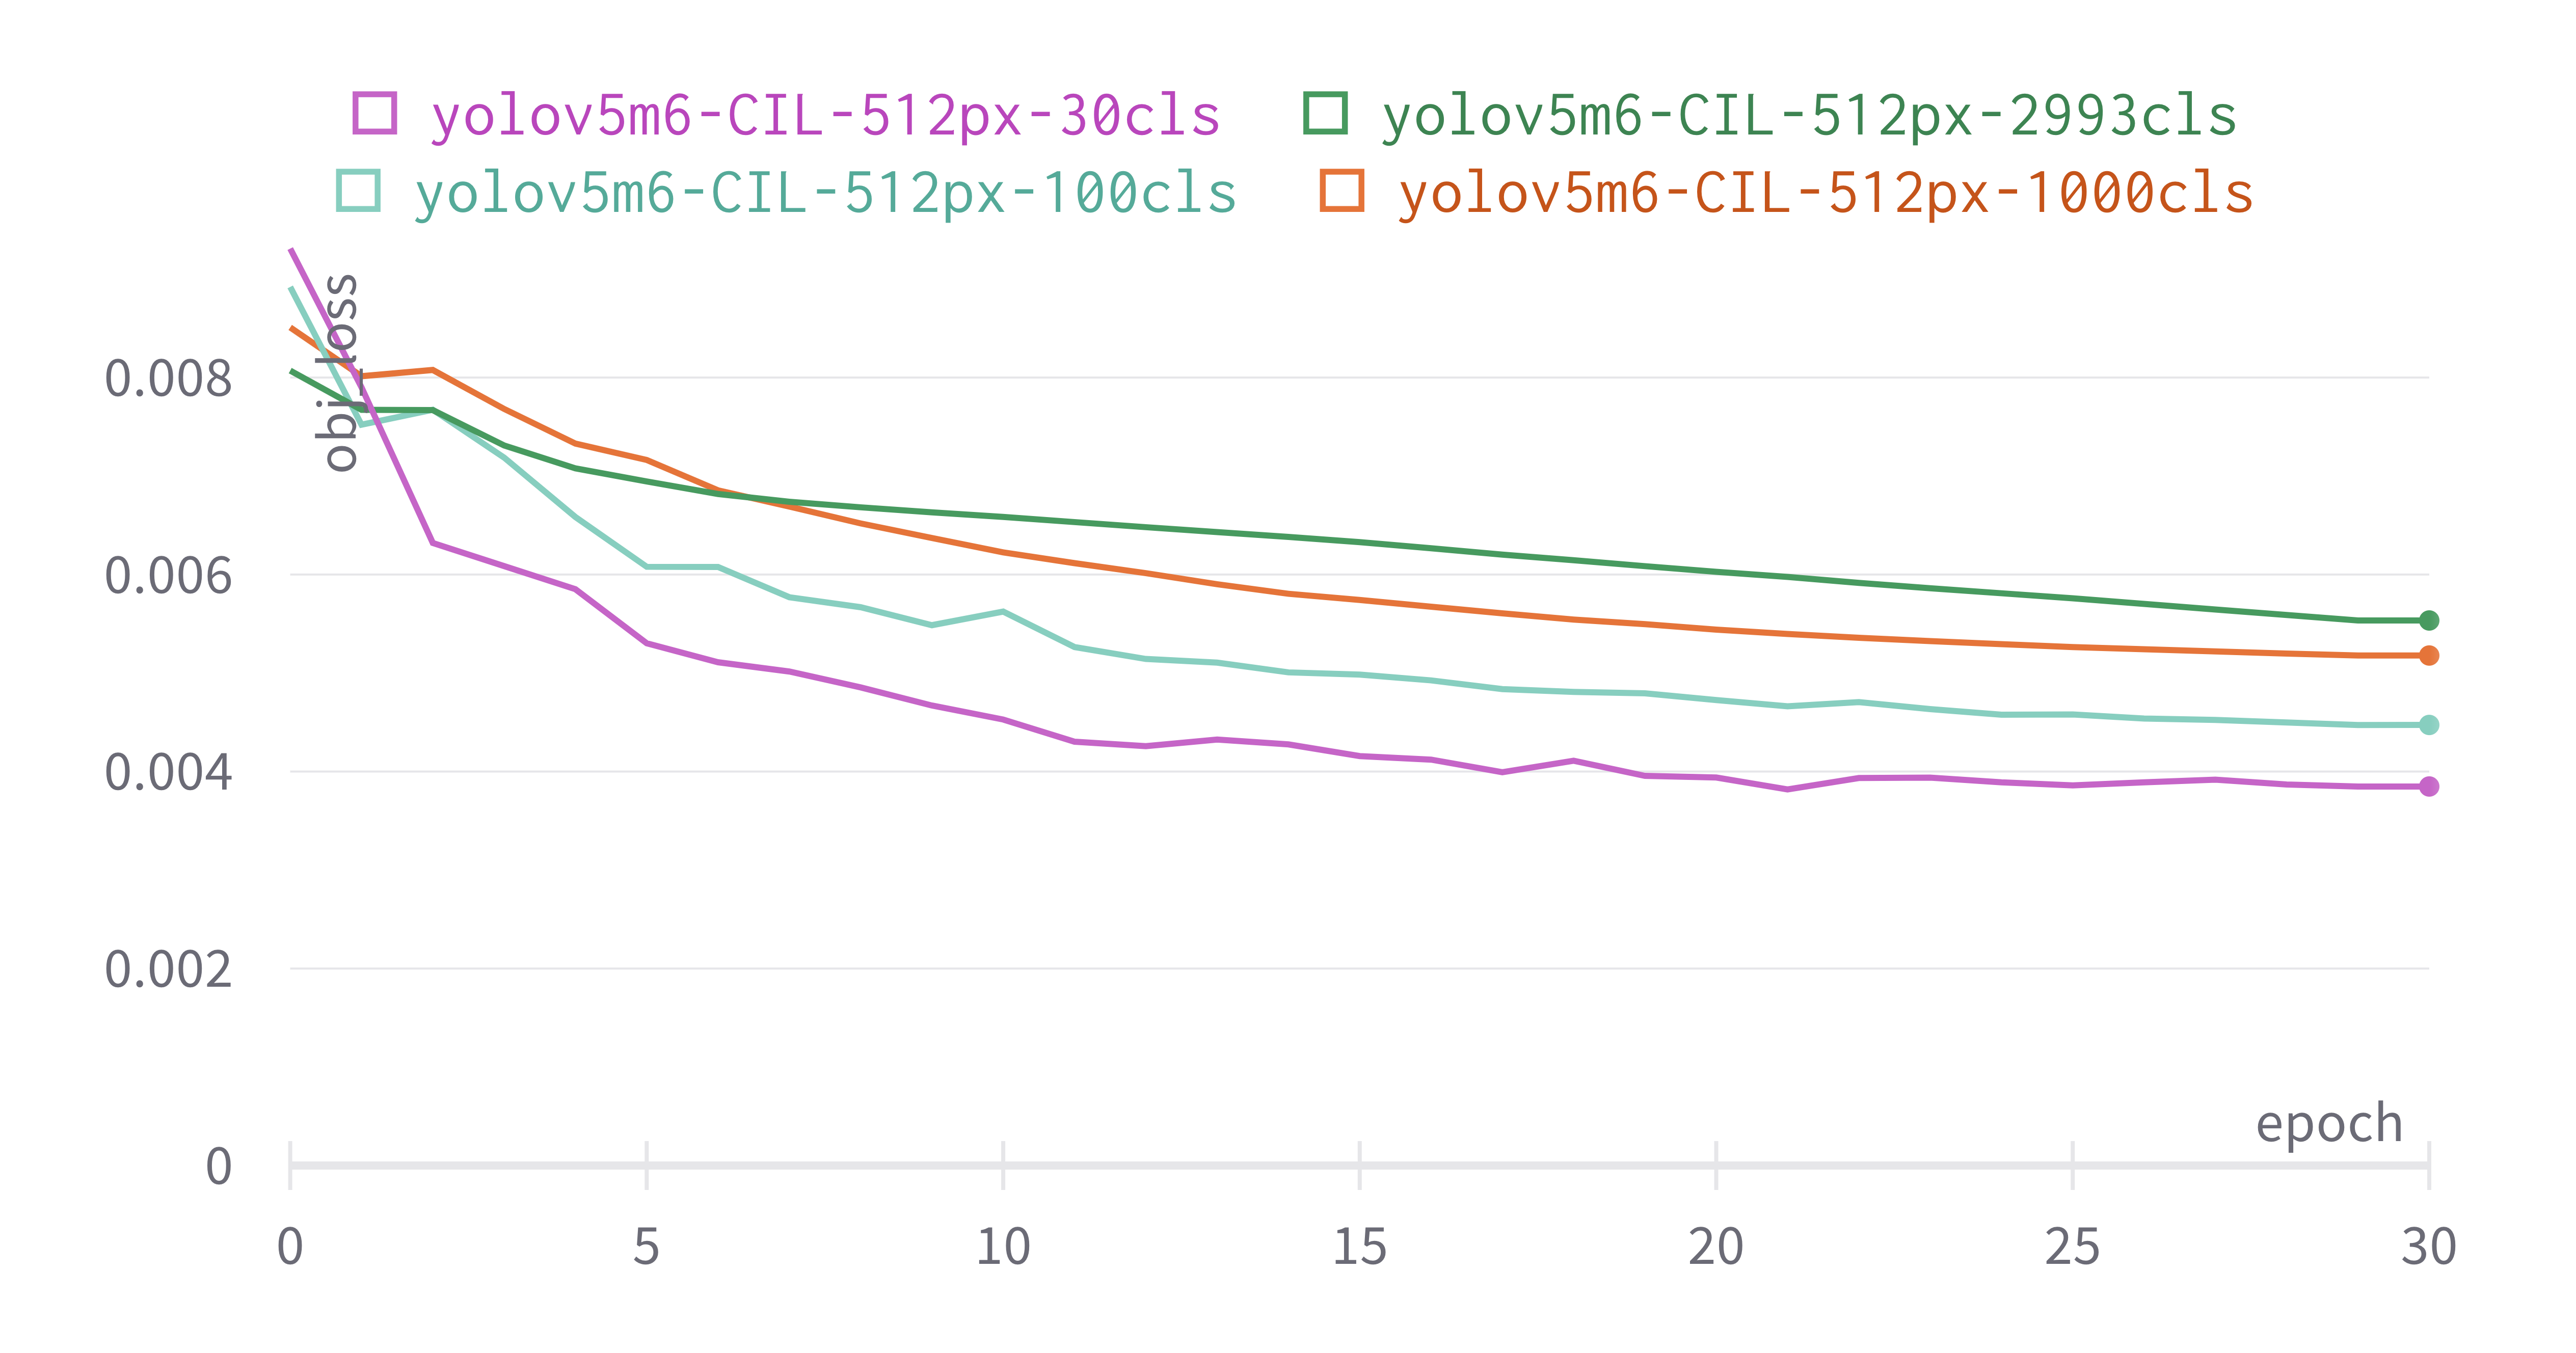
\includegraphics[width=0.50\textwidth]{images/exp/exp-det-obj_loss-2993.png} }}%
    \caption{Performance comparison between the class-agnostic logo detector trained on 1000 classes and the one trained on 2993 classes. The plots show mAP@.5, box loss and object loss on the validation set at each training epoch. Note that these performance are computed on the validation set of each model, thus using 1000 and 2993 classes respectively.}
	\label{fig:exp-det_2993}
\end{figure}


\section{End to end classification}
\label{sec:exp-end2end}
In this last section, the system is tested as a whole.
This consists in combining the first and second step (see \autoref{chap:methods}): the class agnostic logo detection that generates ROIs, and the actual classification performed by the CIL classifier.
Then, the final performance is evaluated considering the precision, recall, mAP@.5 and mAP@.5:.95 on the test set composed of all the 2993 classes.

The model used for the first step of the system is the class agnostic logo detector presented in \autoref{sec:2993-detector}, which is trained using only the 1000 classes used at task 0 by the CIL classifier.

With regard to the CIL classifier, the following models are compared:
\begin{enumerate}
    \item CIL classifier with memory 50 ($\clubsuit$ in \autoref{table:exp6}).
    \item CIL classifier with memory 10 ($\diamondsuit$ in \autoref{table:exp6}).
    \item CIL classifier with memory 50 pruned using learnable masks ($\spadesuit$ in \autoref{table:exp7}).
    \item Student model trained with KD by the CIL classifier with memory 50 ($\heartsuit$ in \autoref{table:exp-kd}).
\end{enumerate}

The results of this evaluation are shown in \autoref{table:exp-end2end}. As a comparison, the results obtained in the literature by Li et al. in SeeTek \cite{li2022seetek} and by Wang et al. in LogoDet-3K \cite{wang2022logodet} (see \autoref{sec:sota-logoyolo}) are reported in \autoref{table:exp-end2end-sota}. The proposed approach using KD outperforms Logo-Yolo introduced in \cite{wang2022logodet} but achieves lower performance than SeeTek.
Still, it must be considered that SeeTek is an open-set retrieval approach and not an incremental learning approach.
This means that in an open-set retrieval approach, the classification of an input logo is performed by assigning the class of the nearest logo in a latent space. By doing so, if an input logo is similar, but does not actually match the training images, it is still recognized, but the system will not be able to integrate new knowledge to recognize new logos.

As we can see from \autoref{table:exp-end2end-sota} and \autoref{table:exp-det_2993}, the end-to-end performance obtained by SeeTek (70.46\% mAP@.5) is very similar to that obtained by the proposed class agnostic logo detector ignoring the classification step performed by the CIL model (70.60\% mAP@.5). This is a clear indication that the detector is a bottleneck for final performance. To asses this problem, a yolo-based detector with a larger number of parameters could be used (e.g. YOLOv5x6 in \autoref{table:yolo-sizes}) or a detector based on transformer architecture could be tested (as proposed by Carion et al. in \cite{carion2020end}).

\begin{table}[H]
    \centering
    \begin{tabular}{c|c|c|c|c}
        \hline
        \textbf{CIL classifier} &
        \textbf{Precision} &
        \textbf{Recall} &
        \textbf{mAP@.5} &
        \textbf{mAP@.5:.95} \\
        \hline
        \hline
CIL\_classifier-mem50 $\clubsuit$&0.578&0.615&0.614&0.417\\
CIL\_classifier-mem10 $\diamondsuit$&0.545&0.591&0.583&0.397\\
Pruned\_CIL\_classifier-mem\_50 $\spadesuit$&0.496&0.485&0.489&0.347\\
KD\_classifier-mem\_50 $\heartsuit$&0.558&0.604&0.59&0.403\\
\hline
\end{tabular}
\caption{End-to-end performance of the system using the class-agnostic logo detector and different CIL classifiers. The Precision, Recall, mAP@.5 and mAP@.5:.95 are computed on the test set composed of all the 2993 classes.}
    \label{table:exp-end2end}
\end{table}


\begin{table}[H]
    \centering
    \begin{tabular}{c|c}
        \hline
        \textbf{Model} &
        \textbf{mAP@.5 (\%)}\\
        \hline
        \hline
SeeTek \cite{li2022seetek}&\textbf{70.46}\\
LogoDet-3K \cite{wang2022logodet}&52.28\\
\hline
Proposed model w/o KD $\clubsuit$&61.40\\
Proposed model with KD $\heartsuit$&59.00\\
\hline
\end{tabular}
\caption{End-to-end performance comparison on LogoDet-3K comparing two SOTA approaches proposed in the literature.}
    \label{table:exp-end2end-sota}
\end{table}
